\RequirePackage{fix-cm}

\documentclass[twocolumn]{svjour3}          % twocolumn
%
\smartqed  % flush right qed marks, e.g. at end of proof
%
\usepackage{graphicx}
\usepackage{cite}
\usepackage{amsmath,amssymb,amsfonts}
\usepackage{algorithmic}
\usepackage{stfloats}
\usepackage{subfig}
\usepackage{float}
\usepackage{multirow}
\usepackage{multicol}
\usepackage{enumitem}
\usepackage{xcolor}
\usepackage{romannum}% for approach #1 and #2
\usepackage{textcomp}
\usepackage[utf8]{inputenc}

\begin{document}

\title{XTNSR: Xception-Based Transformer Network for Single Image Super Resolution%\thanks{Grants or other notes
}

\author{A\textsuperscript{1}\and
        B\textsuperscript{2} \and 
	C\textsuperscript{3}
}

\institute{A\textsuperscript{1} \at
              A, \\
	   A, \\
	   A  \\
           \and
           B\textsuperscript{2} \at
              B, \\
	   B,  \\
	   B,  \\
	   B. \\
	   \email{B@example.com}
	\and
           C\textsuperscript{3} \at
              C, \\
	   C, \\
	   C. \\	   
	   \email{C@example.com}
}
\date{Received: date / Accepted: date}
% The correct dates will be entered by the editor

\maketitle


\begin{abstract}
Single Image Super Resolution has significantly advanced by utilizing Transformers-based Deep Learning algorithms. However, challenges still need to be addressed in handling grid-like image patches with higher computational demands and addressing issues like over-smoothing in visual patches. This paper presents a Deep Learning model for single-image super-resolution. It introduces a novel Local Feature Window Transformer Block and combines it with the Xception Block in a multi-path backbone. With the help of this hybrid architecture, fine-grained features and intricate spatial dependencies can be captured to improve the quality of low-resolution images. An input Patch Embedding layer handles image patches and lowers the computational complexity. The long-range dependencies in the image can be effectively captured using the Local Feature Window Transformer blocks. Xception blocks are used to capture hierarchical features using depth-wise separable convolutions. Additionally, local and global features are efficiently combined when these blocks are integrated into a newly introduced Multi-Layer Feature Fusion Block via skip connections. The experimental results show better performance in Peak signal-to-noise ratio (PSNR), Structural Similarity Index Measure (SSIM), and visual quality than the state-of-the-art techniques. By optimizing parameters, the suggested architecture also lowers computational complexity. Overall, the architecture presents a promising approach for advancing image Super-Resolution capabilities.


\keywords{Single Image super-resolution \and Local Feature Window Transformer Block \and Multi-Layer Feature Fusion Block \and Xception Block}
\end{abstract}

\section{Introduction}
\label{intro}
Image super-resolution (ISR) is a fundamental challenge that aims to recover high-resolution details from lower-resolution images. Deep Learning (DL) models have significantly improved ISR's capabilities. The need for higher image resolution is motivated by its many applications, such as medical image analysis [1], forensics [2], and astronomical imagery [3].
Single-image super-resolution (SISR) is an ill-posed problem because of the generation of multiple High-Resolution (HR) images for every Low-Resolution (LR) image. Many architectures have contributed significantly to Super- Resolution in the Deep Learning panorama, each with advantages. With varying applicability in image segmentation [4], reconstruction [5], estimation [6], anomaly detection [7], etc., these architectures recover the finer detail of any image.

\begin{figure}
  \centering
  \subfloat{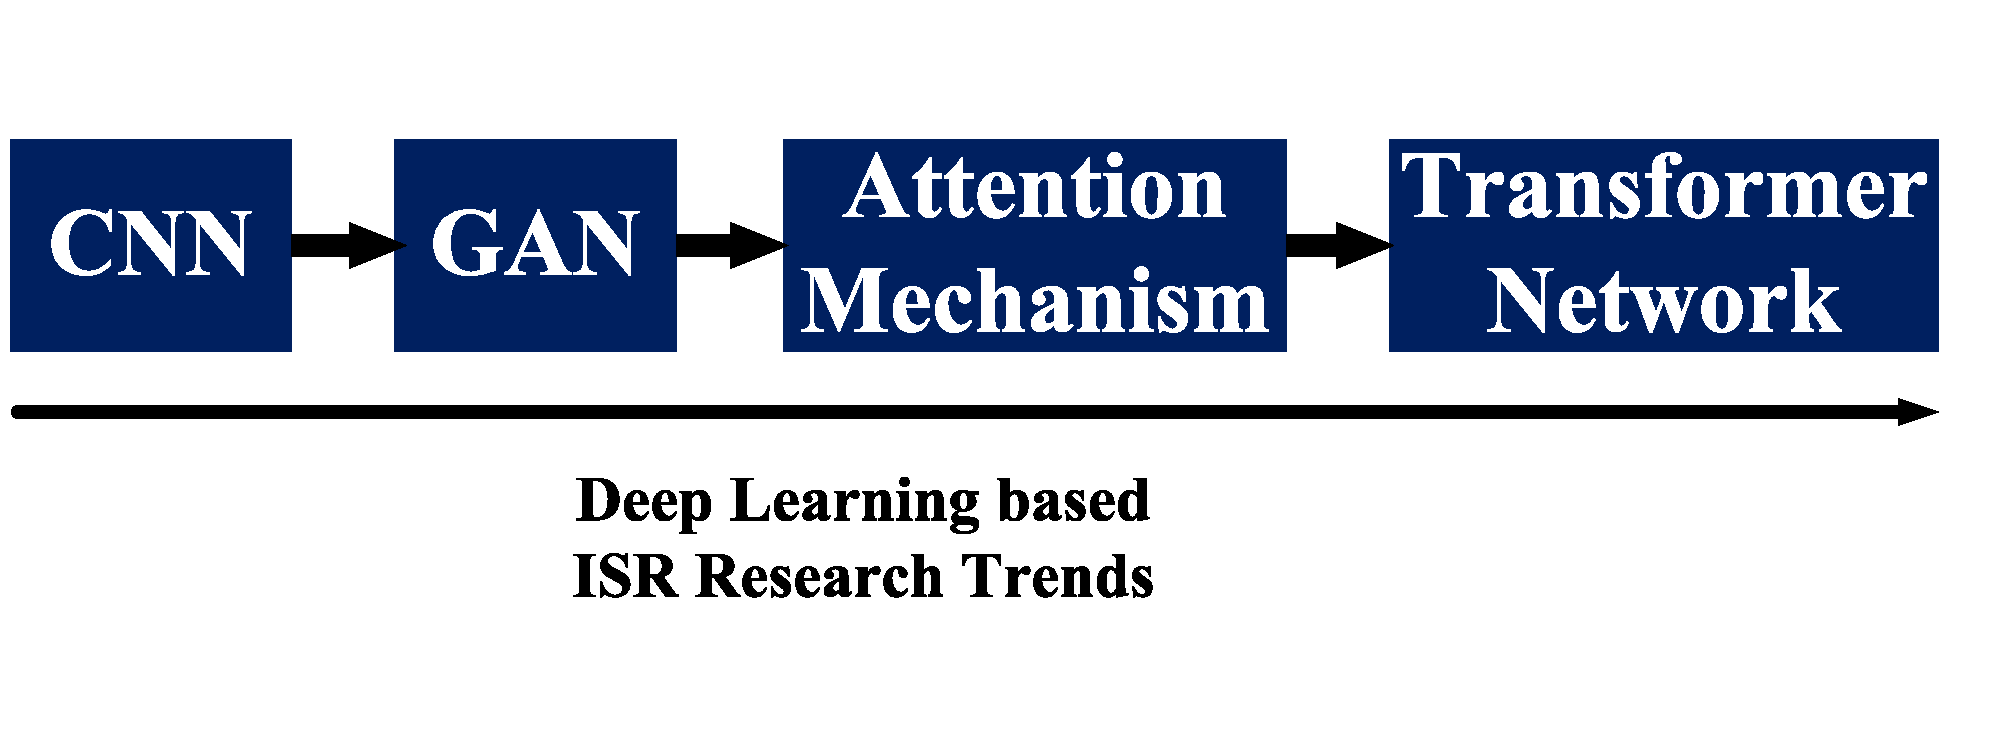
\includegraphics[width=0.5\textwidth]{1FIGURE.pdf}}
   \caption {Research Trends followed by Deep Learning based Image Super-Resolution Methods.}
    \label{fig:1}
\end{figure}
 
Convolutional Neural Networks (CNNs) have led the way regarding image-related tasks. Dong et al. [8] were the first to propose a three-layer (extraction, mapping, and reconstruction) shallow convolutional neural network-based architecture named Super-Resolution Convolution Neural Networks (SRCNN). Other models followed the SRCNN [8] model, like Accelerating the super-resolution convolutional neural network (FSRCNN) [9] to improve training efficiency. Deeper and progressive networks were also introduced for accurate image super-resolution [10; 11; 12; 13; 14; 15; 16; 17] to improve the visual quality of the HR image, increase the model's capacity,  reduce the computational complexity, and enhance the optimization strategy. However, the fundamental issues with conventional CNNs' ability to capture global contextual information and long-range dependencies led to exploring alternative architectures. As seen in Figure 1, the research trends shifted from CNNs to GANs, attention mechanisms, and transformer networks. To obtain more visually pleasing results, the researchers explored the direction of Generative Adversarial Networks (GANs) [18; 19; 20]. While Generative Adversarial Networks (GANs) are incredibly powerful for image generation tasks, their direct application to image super-resolution can sometimes pose challenges, especially regarding training stability and balancing the trade-off between generating realistic high-resolution images and avoiding model collapse. Due to this, the research moved to introduce attention mechanisms in CNNs' which can help the model focus on relevant image regions and capture complex spatial dependencies. Many recent models such as Image super-resolution using very deep residual channel attention networks (RCAN) [21], Image Super-Resolution with Cross-Scale Non-Local Attention and Exhaustive Self-Exemplars Mining (CSNL) [22], Image Super-Resolution with non-local sparse attention (NLSN) [23], Single image super-resolution via a Holistic Attention Networks (HAN) [24] and Efficient long-range network for image super-resolution (ELAN) [25] etc. have shown remarkable performance gains with the addition of different attention mechanisms in CNNs' making it possible to capture fine-grained detail and improve feature extraction. Nevertheless, these models proved to need to be improved when handling grid-like image data. Transformer stands out by leveraging attention mechanisms to capture better global dependencies and handle grid-like image data. The most recent models for demonstrating the efficient use of transformers in ISR are Image restoration using a Swin transformer (SwinIR) [26], Hierarchical Vision Transformer using Shifted Windows (Swin Transformer) [27], and Permuted Self-Attention for Single Image Super-Resolution (SRFormer) [28]. Even though they are cost-effective, there is still room to improve the balance between local and global context and inference time.

In the context of built-in systems and intelligent hardware with immediate handling, the model's size is crucial for attaining faster and more advanced results, particularly when dealing with higher scale factors in image super-resolution. Despite the advancements in state-of-the-art quantitative and qualitative methods, they still need to be improved.

(i) Images with high-resolution grid-like patches can be computationally demanding, resulting in higher memory resource needs and longer inference time. 

(ii) Balancing local and global context while addressing potential issues such as over-smoothing and artifact generation. 

(iii) When dealing with noisy low-resolution images, earlier approaches may introduce rugged patterns and uneven edges and may not effectively recover fine details.

An effective solution to all these issues is to combine the complementary abilities of Transformer [29] and Xception blocks [30] in a multi-path network [31] using skip connections [32]. This approach combines various types of extracted features from each path, enhancing both the output's perceptual quality and the SR model's operation time. It suggests that the network's layers don't need to wait for the results of earlier layers' computations and helps to reduce inference time. The multi-path network was introduced by Kim et al. in DRCN [13] to extract different types of features and combine them for performance enhancement and reduce parametric complexity. 

Making use of a similar approach, we introduce a new Local Feature Window Transformer Block (LFWT) and a Multi-Layer Feature Fusion (MLFF) Block to effectively capture spatial relational features and combine complementary abilities of the Transformer with the Xception block in a multi-path network backbone. Patch embedding helps to address the challenge of processing grid-like image data by transforming input images into smaller patches, reducing the model's complexity. Using Local Feature Window Transformer (LFWT) Blocks in a multi-path framework helps strike a balance between the local and global context to address the issue of over-smoothing.  Integration of the Xception Block via skip connections in a Multi-Layer Feature Fusion (MLFF) Block increases the model’s ability to learn hierarchical features. It helps finely recover images with noise and improves training stability.

To summarize, the following list outlines the main contributions of our proposed method:

(1) Patch Embedding layer addresses scalability challenges, balancing computational efficiency and accuracy in adapting to varied computational resources. 

(2) The method extracts features using LFWT Block. It processes them in a multi-path network, enabling the model to capture and balance local and global features to mitigate over-smoothing and artifact generation. 

(3) Extracting hierarchical features from the Xception Block and integrating them in the MLFF Block helps recover fine details from noisy images, thus reducing noise.  

The remaining sections of the article are organised as follows. Section II states the related work, Section III presents the proposed network architecture methodology, and Section IV demonstrates the experimental evaluations, ablation analysis, and visual results on experimental datasets. Finally, Section V gives conclusion, and recommendations for further work.

\section{Related Work}

In recent years, brilliant success in Single Image Super-Resolution has been driven by the ongoing development of deep learning architectures and techniques. This section summarizes the major contributions made to the field, with an emphasis on models that are similar to our suggested approach, including Xception blocks [30], transformer [29], patch embedding [33, 34], and multi-path networks [31].

The pioneering work in the field of image Super-Resolution using the power of convolutional neural network was done by Dong et al. [8], which introduces a three-layered network for extraction features from low-dimensional space and mapping them to reconstruct higher dimensional space. SRCNN [8] was a remarkable introduction to Deep Learning Image Super-Resolution models. After this, much research was done to improve the deep learning models regarding performance, computational complexity, training efficiency, and stability. The better version of SRCNN [8] was later introduced by Dong et al. to reduce the computational complexity named FSRCNN [9]. While improving the deep learning algorithms, the researchers mainly focused on improving the methods regarding model frameworks, up-sampling methods, network designs, and learning strategies. Even though FSRCNN [9] improved the network's computational complexity, it still had limited capacity. The research shifted to creating deeper and more intricate architectures to improve the model capacity. A 20-layer residual network named VDSR [10] was introduced by Kim et al., and a pyramid structure network LapSRN [12] was proposed by Lai et al. Though the deeper network significantly improved performance, they had high computational costs. By introducing the recursive learning strategy in its network design, Kim et al. improved the deeper network introduced by DRCN [13] and rectified the concept of deeper networks. To further improve the training convergence, DnCNN [11] was introduced by Chen et al. Since the deeper network could not meet the demand for current cutting-edge devices, lightweight models such as IMDN [35] by Hui et al. and DRRN [14] by Tai et al. were introduced. When the progress shifted towards improving residual networks and introducing EDSR [17], substantial gains in performance were made, and the training efficiency of the model was boosted. EDSR [17] won the NTIRE (2017) challenge and became the widely used backbone of current research for creating Deep Learning Image Super-Resolution methods. To fit in the memory resources needed for the algorithms, a persistent memory network for Image Super-Resolution MemNet [15] was introduced by Tai et al. Another feedback network, the Super Resolution Feedback Network (SRFBN) [36], was also introduced to use fewer trainable parameters. To deal with noisy image methods such as SRMDNF [37] performed significantly great. Shallower Networks were also adapted to reduce the computational requirements, such as Super Sampling Network (SSNet) [38] by Hung et al. and Deep Recurrent Fusion Network (DRFN) [39]. Another approach that focused on quantization and compression technique was also introduced by Muhammad et al. in Squeeze-and-Excitation Next for Single Image Super-Resolution (SENext) [40].

Although all these techniques performed better in quantitative measurements, the visual quality could have been significantly improved. Hence, to improve the visual patches of the images, the research trend shifted to Generative Adversarial Networks (GANS). SRGAN [18], EnhanceNet [19], and ESRGAN [20] are some good examples of GAN networks and have demonstrated significant visual gains in Image Super-Resolution. However, GANs showed great enhancement in the visual performance but were insufficient to generate better PSNR values. Hence, the Mean Opinion Score (MOS) [41], a manual estimate of human raters to measure the performance of the GAN model, was introduced. The research again shifted to the neural network when attention mechanisms were introduced in the Convolutional Neural Networks (CNNs), overcoming the drawbacks of both earlier approaches. 

Attention mechanisms have greatly enhanced super-resolution models for images. Combining attention mechanisms and convolutional operations has demonstrated improved performance. Zhang et al. Residual Dense Network (RDN) [42] showcases the efficacy of integrating skip connections and residual learning for enhanced feature extraction and super-resolution quality. Works like Residual Attention Network (RAN) [43] by Wang et al. and Image Super-Resolution Using Very Deep Residual Channel Attention Networks (RCAN) [21] by Zhang et al. demonstrate the benefits of attention mechanisms when focusing on informative image regions. Since then, many works have been contributed with the use of different types of attention mechanisms, such as Image Super-Resolution with Cross-Scale Non-Local Attention and Exhaustive Self-Exemplars Mining (CSNL) [22], which used non-local attention and combined it with cross-scale features. Another similar work was introduced in Multi-FusNet of Cross Channel Network for Image Super-Resolution (MFCC) [44] and Fast Non-Local Attention network for light super-resolution FNLNET [45]. To deal with more intricate features, a second-order channel attention module was introduced in the Second-order Attention Network for Single Image Super-Resolution (SAN) [46]. Spatial Attention was introduced in the Residual Feature Aggregation Network (RFANet) [47]. Channel Split Image Super-Resolution (CSISR) [48] was introduced to improve learning capability. Another lightweight model to reduce the computational requirements was introduced in the Dynamic Residual Self-Attention Network (DRSAN) [49]. For larger and contextual information, Context Reasoning Attention Network (CRAN) [50] and Information Growth Attention Network (IGAN) [51] were introduced. To better understand the correlation between layers and features and improve performance, a Holistic Attention Network (HAN) [24] was introduced. Sparsity, along with non-local attention, was also introduced to improve the computation complexity and preserve model capabilities in Non-Local Neural Networks (NLNN) [52] and Image Super-Resolution using Non-Local Sparse Attention Networks (NLSN) [23]. Architectural changes were made using the U-Net framework to non-local design to improve performance further and reduce computational burden in the Deep Attention Network for Single Image Super-Resolution (DANS) [53]. Although attention mechanisms have proven to better understand the complex contextual and finer details, improvement is still needed.

Patch embedding was first introduced in Attention is All You Need by Vaswani et al. [54], significantly improving performance when applied to attention mechanisms. This concept was introduced from patch embedding in transformers. Transformer-based models have become more popular for tasks involving image super-resolution. In their introduction of the Image Transformer, Dosovitskiy et al. [29] emphasized that transformers could capture long-range image dependencies. However, challenges persist in efficiently processing grid-like image structures, prompting the need for innovative architectural solutions. Since Transformer architectures have shown great success in Natural Language Processing (NLP) [55], their contribution to image super-resolution also achieves greater gain in qualitative and quantitative measures. The pioneering work of Vision Transformer (ViT) [29] has led to many developments in Image Super-Resolution using transformers. After that, much work in image super-resolution has been depicted using transformers. One is Image Restoration Using a Swin Transformer (SwinIR) [26]. It uses a fixed window size of 8 × 8 for extracting features simplified in the Efficient Long-Range Attention Network for Image Super-resolution (ELAN) [25] by different window sizes to improve self-attention in transformers showing better performance gains. Furthermore, improvements are shown in Hierarchical Vision Transformer using Shifted Windows (Swin Transformer) [27], which used the shifted window technique instead of sliding window to make the processing of image patches more compact. Recently, Permuted Self-Attention for Single Image Super-Resolution (SRFormer) [28] has been introduced, which performs self-attention in large window sizes to further improve the performance without increasing the computational cost of the model. 

Chollet et al. introduced deep Learning with Depthwise Separable Convolutions (Xception) [30]. It showed the efficacy of its customary design, which enhanced parameter efficiency and feature extraction capabilities by replacing depth-wise separable convolutions for conventional convolutional layers. The use of Xception for single-image super-resolution was extended by Lim et al. in Enhanced Deep Residual Networks for Single Image Super-Resolution (EDSR) [17]. By incorporating Xception blocks into the network, the study demonstrated enhanced feature extraction, making it easier to collect hierarchical information for reconstructing high-resolution images. As computational complexity decreased, Xception's depth-wise separable convolutions [30] assisted in preserving performance. Xception has demonstrated success in various image-processing tasks combined with other neural network components in hybrid architectures. Zhang et al. in Residual Dense Network (RDN) [42] demonstrated the advantages of combining depth-wise separable convolutions with residual learning for better super-resolution quality.

Significant progress has been made in image super-resolution using transformer-like architectures. Still, there is a need for techniques that can handle grid-like image data effectively while requiring less processing power. Furthermore, searching for the optimal possible balance between local and global information is still necessary to achieve realistic super-resolved results while mitigating general artifacts and over-smoothing. Research is still being conducted to address issues like computational efficiency and cross-domain generalization. Reaching the maximum potential of super-resolution images for a range of uses, such as multimedia [56], live streaming [57], medical [58], security [59],  and super-resolution images in real time [60].

\section{Proposed Method}

This section introduces our unique method for image super-resolution, which involves integrating a novel Local Feature Window Transformer (LFWT) Block and the Xception block into a multi-path framework and applying patch embedding at the input side. Patch embedding reduces the complexity of the model by transforming input images into smaller patches, which helps to address the difficulty of processing grid-like image data. To address the issue of over-smoothing, a multi-path framework that uses Local Feature Window Transformer (LFWT) Blocks helps to balance the local and global context. When the Xception Block is integrated into a Multi-Layer Feature Fusion (MLFF) Block through skip connections, the model's capacity to learn hierarchical features is enhanced, and it also aids in the fine recovery of noisy images and enhances training stability.
The architecture of the Xception-Based Transformer Network for SISR (XTNSR) in Figure 2 (a) consists of six Local Feature Window Transformer (LFWT) Blocks and four Xception blocks connected in a multi-path framework. The initial features are extracted using a standard 3 × 3 convolution following the patch embedding at the input side. It utilizes six paths for input flow: Dense Feature Path for dense feature transmission and Shallow Feature Path for shallow features. Dense features traverse through three Dense Feature Paths (D1, D2, D3), and shallow features traverse through three shallow feature paths (S1, S2, S3). These features are fused in the Multi-Layer Feature Fusion (MLFF) Block. Finally, all features pass through the deconvolution layer for HR image reconstruction.

\begin{figure*}
    \centering
    \includegraphics[width=\linewidth]{2Figure.pdf}
    \caption{The design of the suggested network structure of the Xception-Based Transformer Network for Single Image Super-Resolution (XTNSR).}
    \label{fig:2}
\end{figure*}

\subsection{Initial Feature Extraction and Patch embedding}
Figure 2 (a) shows that the input's initial features are extracted using a normal 3 × 3 convolution, and then patch embedding is applied to the convoluted input. Equation 1 demonstrates the initial feature extraction stage. 

\begin{equation}
{H_{0}}= {H_{Conv}}({H_{LR}}),
\end{equation}

Here, ${H_{Conv}}$$(.)$ represents a 3 $\times$ 3 convolution operation. ${H_{LR}}$ is the input Low-Resolution (LR) image, fed to the normal convolution for extracting initial features, and ${H_{0}}$ is the output of the convolution layer. 


\begin{equation}
{H_{P}}= {P_{embed}}({H_{0}}),
\end{equation}

${P_{embed}}$$(.)$ represents Patch Embedding, and ${H_{P}}$ results from embeddings obtained after applying Patch embedding. After obtaining the initial features, patch embedding is applied on ${H_{0}}$, as depicted in Equation 2. Equation 2, depicts the Patch embedding over the convoluted output. The higher-dimensional embeddings obtained are input tokens to the subsequent Transformer. They help retain spatial information by capturing local patterns within each patch. The embedding tokens have sequence lengths of \textit{L} and \textit{P} as embedding dimension. 

\subsection{Local Feature Window Transformer Block (LFWT)}
The Local Feature Window Transformer (LFWT) Block is constructed using the Shifted Window Multi-head Self-Attention (SW-MSA) [27] module and the Multi-layer Perceptron (MLP) [61] with Rectified Linear Unit (ReLU) [62] activation. Each module applies a layer norm (LN) before the MLP and SW-MSA modules. Following every module is another residual Skip connection.

\begin{figure}
  \centering
  \subfloat{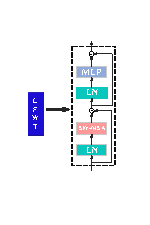
\includegraphics[width=0.5\textwidth]{3FIGURE.pdf}}
   \caption {The design of the Local Feature Window Transformer (LFWT) Block.}
    \label{fig:3}
\end{figure}

As seen in Figure 3, the embeddings from the previous layer are fed to the SW-MSA module present in the LFWT Block, followed by Layer Norm. This module's output is then added to the embeddings passed through the residual connection and transferred to the next MLP module. The output of the MLP module is then added to the summed output of the previous module. Equations 3 and 4 show the SW-MSA and MLP module operation in the LFWT Block.

\begin{equation}
{M_{SWMSA}}= {H_{SWMSA}}({H_{LN}}({H_{I1}})) + {H_{I1}},
\end{equation}

Here,  ${H_{I1}}$ is the input to the Local Feature Window Transformer Block, ${H_{LN}}$$(.)$ is the Layer Norm function, $({H_{SWMSA}})$$(.)$ is the Shifted Window Multi-head Self-Attention function, ${M_{SWMSA}}$  is the output of the SW-MSA module in the LFWT Block.

\begin{equation}
{H_{LFWT}}= {H_{MLP}}({H_{LN}}({M_{SWMSA}})) + {M_{SWMSA}},
\end{equation}

In Equation 4, ${H_{MLP}}$$(.)$ is the output function of the Multi-layer Proton, and ${H_{LFWT}}$ represents the output of the Local Feature Window Transformer (LFWT) Block.

\subsection{Xception Block (X)}

As presented in Figure 4, the Xception Block is designed to be relatively lightweight. The Xception block introduces depthwise separable convolution to make it more computationally efficient and reduces the number of parameters while maintaining strong performance.

It consists of a series of depthwise separable and pointwise convolution combinations followed by ReLU non-linearity. This series combination is then connected in parallel. The output from the two parallelly connected modules is then summed up to obtain the output from the Xception Block. This enables the model to learn hierarchical features within the same layer.

\begin{equation}
\begin{aligned}
    {H_{X}} &= \text{ReLU}\bigl(H_{\text{Conv}}(H_{\text{DWConv}}(H_{\text{SWT}}))\bigr) \\
    &\quad+ \text{ReLU}\bigl(H_{\text{Conv}}(H_{\text{DWConv}}(H_{\text{SWT}}))\bigr),
\end{aligned}
\end{equation}

Here, $H_{\text{DWConv}}$$(.)$ is the Depthwise Separable convolution operation function, ${H_{\text{Conv}}}$$(.)$  is the Pointwise convolution operation function, ${ReLU}$$(.)$ represents the non-linearity, and ${H_{X}}$ represents the output of the Xception Block.

\begin{figure}
  \centering
  \subfloat{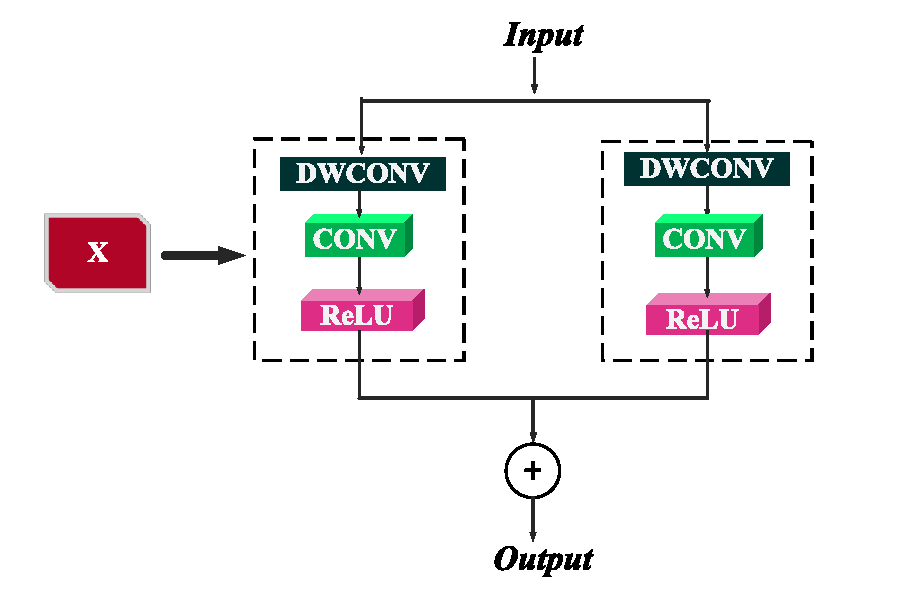
\includegraphics[width=0.5\textwidth]{4FIGURE.pdf}}
   \caption {Xception Block (X).}
    \label{fig:4}
\end{figure}

Including Xception Block and Transformers in a multi-path framework allows the network to balance an image's local and global details. Since the Xception Block operates both spatial and channel dimensions simultaneously. It also incorporates residual connections to help with the flow of gradients during training and mitigate the vanishing gradient problem. 

\subsection{Multi-Layer Feature Fusion Block (MLFF)}

As seen in Figure 5, the Multi-Layer Feature Fusion Block (MLFF) is designed to merge features from the multiple paths present in the network. This block helps to merge the dense and shallow features transferring through different paths in the network. It concatenates the features from multiple paths, and then the fused features pass through the Depthwise Separable convolution followed by a Fully Connected layer. After that, the feature is passed through a residual connection and a ReLU non-linearity and fused again to pass through the Fully Connected layer. It helps to point the spatial region information from different paths in a network. Furthermore, it creates a multi-path representation of the input image and highlights the important features that contribute to improving the model's performance. Finally, all the features are aggregated and passed through a deconvolution layer to generate the High-Resolution image.

\begin{figure}
  \centering
  \subfloat{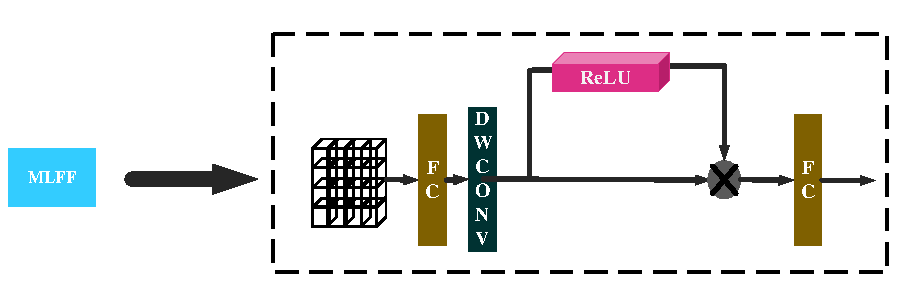
\includegraphics[width=0.5\textwidth]{5FIGURE.pdf}}
   \caption {Multi-Layer Feature Fusion Block (MLFF).}
    \label{fig:5}
\end{figure}

Equations 6, 7, 8, 9, and 10 stepwise describe how the Multi-Layer Feature Fusion (MLFF) Block merges the features from multiple paths in the network. As the features from multiple paths enter the MLFF block, they are concatenated, as shown in Equation 6.

\begin{equation}
{MLFF_{Cat}}= {cat}({H_{S1}},{H_{S2}},{H_{S3}},{H_{D1}},{H_{D2}},{H_{D3}}),
\end{equation}

In Equation 6, ${MLFF_{Cat}}$ denotes the output of the concatenation of features from multiple paths in the MLFF Block, ${cat}$$(.)$ is the concatenation operation, ${H_{S1}},{H_{S2}},{H_{S3}},{H_{D1}},{H_{D2}}, and {H_{D3}}$ are the shallow and dense features from paths S1, S2, S3, and dense feature paths D1, D2, and D3. 

After this, these concatenated features are passed through a Depthwise Separable convolution layer and a Fully Connected layer to reduce the computational burden.

\begin{equation}
{MLFF_{DW}}= {H_{DWConv}}({H_{FC}}({MLFF_{Cat}})),
\end{equation}

In Equation 7, ${H_{FC}}$$(.)$ is the Fully Connected layer function, ${MLFF_{DW}}$ is the result obtained in the MLFF Block by the Depthwise Separable convolution.

The generated features are concatenated together after applying the non-linearity and residual connection.

\begin{equation}
{MLFF_{FC}}= {cat}({ReLU}({MLFF_{DW}}), {MLFF_{DW}}),
\end{equation}

${MLFF_{FC}}$, as seen in Equation 8, is the input of the last Fully Connected layer in the MLFF Block.

The concatenated output is then passed to the Fully Connected layer to better generalize the data.

\begin{equation}
{MLFF_{O}}= {H_{FC}}({MLFF_{FC}}),
\end{equation}

${MLFF_{O}}$ in Equation 9 is the output of the MLFF Block.

Finally, the Multi-Layer Feature Fusion Block (MLFF) output is fed to the deconvolution layer to reconstruct the high-resolution image.

\begin{equation}
{HR_{O}}= {H_{DConv}}({MLFF_{O}}),
\end{equation}

Lastly, in Equation 10, ${H_{DConv}}$$(.)$ is the deconvolution operation, and ${HR_{O}}$ is the generated high-resolution output.

\section{Experimental Findings}

Our proposed XTNSR model's performance was verified through experiments conducted on benchmark test datasets, resulting in quantitative and qualitative visual results. Analysis based on average PSNR (dB) SSIM has also been graphically demonstrated for state-of-the-art methods. Additionally, this section discusses the computational cost in terms of execution time and network parameters. Analysis for different numbers of Local Feature Window Transformers (LFWT) and Xception Block has also demonstrated which combinations give the best qualitative and quantitative results. Furthermore, time and space complexity analysis with different state-of-the-art models is also shown. Moreover, the ablation analysis includes the Flops v/s PSNR computation, the results of changing the LFWT Block's window size during testing, comparison with traditional denoising methods to show the model's performance on noisy images,  changing the non-linearity function in the Xception and Multi-Layer Feature Fusion (MLFF) Block, its PSRN and SSIM convergence, and loss analysis. 

\subsection{Experiment Configuration}
This section presents the datasets, evaluation metrics, and training specifics used to test and train our suggested structure on publicly available datasets. It is mentioned that the testing and training sets are different.

\subsubsection{Datasets} 
The DIV2K [63] dataset has been used for network training and validation. DIV2K [63] is divided into 800 high-quality images, 100 validation images, and 100 test images for the training phase. Out of these 1000 images, we have used 800 images for training. We tested using five benchmark datasets: Set5 [64], Set14 [65], BSD100 [66], Manga109 [68], and Urban100 [67].

\subsubsection{Evaluation Metrics} 
For a fair comparison with earlier research, the standard metrics Peak Signal-to-Noise Ratio (PSNR) (dB) and the structural similarity index (SSIM) were calculated for quantitative measures. Equations 11 and 12 show the mathematical expression of PSNR and SSIM measures.
\begin{equation}
\text{PSNR} = 10 \cdot \log_{10}\left(\frac{M^2}{\frac{1}{N} \sum_{j=1}^{N} (I_{G}(j) - {\hat{I}_{S}}(j))^2}\right),
\end{equation}

Here, PSNR is the Peak Signal-to-Noise Ratio measured in decibels (dB), M is the maximum pixel value having N number of pixels, ${I_{G}}$ is the ground truth image, and ${\hat{I}_{S}}$ is the reconstructed image.

\begin{equation}
\text{SSIM}(I; \hat{I}) = \left[ \text{C}_{l}(I; \hat{I}) \right]^\alpha \left[ \text{C}_{c}(I; \hat{I}) \right]^\beta \left[ \text{C}_{s}(I; \hat{I}) \right]^\gamma,
\end{equation}

Here, SSIM represents the Structural Similarity Index, $I$, is the ground truth image, $\hat{I}$ is the reconstructed HR image, $\alpha$, $\beta$, $\gamma$ are exponents that control the relative importance of the luminance, contrast, and structure, and ${C}_{l}$, ${C}_{c}$, ${C}_{s}$ are the luminance, contrast, and structure.

\subsubsection{Training and Testing Specifics}

To train our model, we used 48 $\times$ 48 low-resolution patches. The window size is chosen to be 24 $\times$ 24. MATLAB R2022b was used to create low-resolution images for scale $\times$2, $\times$3, $\times$4, and $\times$8. An NVIDIA GeForce GTX 2080ti GPU with 24GB of RAM is used to train the suggested network. The proposed model's algorithm was coded using the programming language Python 3.6 and the platform PyTorch 1.7.0. Eight hundred samples are taken from the DIV2K [63] dataset for model training. We use an Adam optimizer with $\beta_1 = 0.90$ and $\beta_2 = 0.99$ for optimization. Every 200 epochs, the learning rate of the suggested model is halved and maintained at 10$^{-4}$. The model has been trained for 1000 iterations.
Five common benchmark datasets, namely Set5 [64], Set14 [65], BSD100 [66], Urban100 [67], and Manga109 [68], were used to test our suggested model. Bicubic kernels are used to downsample the HR images to produce the LR image. The window size during testing is also set for 24 $\times$ 24. The training samples are randomly cropped into 48 $\times$ 48 patches, and the batch size of training images is set as 4. Additionally, data augmentation generates additional samples for the algorithm through random rotation and flipping for 90, 180, and 270 degrees.

\subsection{Evaluations based on quantitative metrics in state-of-the-art methods}
The standard quantitative metric comparison of five benchmark test datasets for scale factors $\times2$, $\times3$, $\times4$, and $\times8$  is presented in Table 1. We have used 16 state-of-the-art algorithms widely accepted for Single Image Super-Resolution, including Bicubic, SRCNN [8], FSRCNN [9], VDSR [10], MemNet [15], LapSRN [12], SENext [40], RCAN [21], MFCC [44], EDSR [17], HAN [24], NLSN [23], ESRT [64], SwinIR [26], ELAN [25], and SRFormer [28] to show comparison with our proposed XTNSR. Regarding  PSNR and SSIM, our suggested XTNSR analytical outcomes have considerably surpassed the state-of-the-art techniques. In addition, our suggested approach outperformed other SOTA models in terms of PSNR and SSIM on all averages for benchmark datasets.

\begin{table*}
\caption{Standard metric assessment of our suggested XTNSR against state-of-the-art SR methods for up-scaling factors $\times 2$, $\times 3$ $\times 4$, and $\times 8$. The highest score is bolded and colored {\color{red}\textbf{Red }}. The second-greatest score is highlighted and displayed in {\color{blue}\underline{Blue}}.}

\label{table1}
\setlength{\tabcolsep}{2 pt}
\begin{tabular}{|c|c|c|cc|cc|cc|cc|cc|cc|}
\hline
\multirow{2}{*}{Method} & \multirow{2}{*}{Factor} & \multirow{2}{*}{\#Param}& \multicolumn{2}{c|}{Set5 [64]}& \multicolumn{2}{c|}{Set14 [65]}& \multicolumn{2}{c|}{BSD100 [66]}& \multicolumn{2}{c|}{Urban100 [67]}& \multicolumn{2}{c|}{Manga109 [68]}& \multicolumn{2}{c|}{Average}\\


 \cline{4-15}&&& \multicolumn{1}{c|}{PSNR$\uparrow$}  & SSIM{$\uparrow$}   & \multicolumn{1}{c|}{PSNR$\uparrow$}  & SSIM {$\uparrow$}   & \multicolumn{1}{c|}{PSNR$\uparrow$}  & SSIM {$\uparrow$}   & \multicolumn{1}{c|}{PSNR$\uparrow$}  & SSIM {$\uparrow$}  & \multicolumn{1}{c|}{PSNR$\uparrow$}  & SSIM {$\uparrow$}   & \multicolumn{1}{c|}{PSNR$\uparrow$}  & SSIM {$\uparrow$}  \\
 \hline

Bicubic&$\times2$ & -/-& \multicolumn{1}{c|}{33.68 } & 0.9304  & \multicolumn{1}{c|}{30.24 } &0.8691  & \multicolumn{1}{c|}{29.56 } & 0.8435  & \multicolumn{1}{c|}{26.88 } & 0.8405  & \multicolumn{1}{c|}{31.05 } & 0.9349&
\multicolumn{1}{c|}{30.23} & 0.8832 \\


SRCNN [8] & $\times 2$ & 57K& \multicolumn{1}{c|}{36.66 } & 0.9542  & \multicolumn{1}{c|}{32.45 } & 0.9067  &\multicolumn{1}{c|}{31.36 } & 0.8879  & \multicolumn{1}{c|}{29.51 } &0.8946 & \multicolumn{1}{c|}{35.72} &0.9680
&\multicolumn{1}{c|}{33.11} & 0.9219\\

FSRCNN [9]& $\times 2$& 12K & \multicolumn{1}{c|}{36.98} &0.9556& \multicolumn{1}{c|}{32.62} & 0.9087 &\multicolumn{1}{c|}{31.50} &0.8904& \multicolumn{1}{c|}{29.58} &0.9009& \multicolumn{1}{c|}{36.62} &0.9710
&\multicolumn{1}{c|}{33.56} & 0.9260\\

VDSR [10]& $\times 2$&665K& \multicolumn{1}{c|}{37.53} & 0.9587 & \multicolumn{1}{c|}{33.05} & 0.9127 &\multicolumn{1}{c|}{31.90} & 0.8960& \multicolumn{1}{c|}{30.77} & 0.9141 & \multicolumn{1}{c|}{37.16} & 0.9740
&\multicolumn{1}{c|}{33.24} & 0.9314\\

MemNet [15] & $\times 2$&677K& \multicolumn{1}{c|}{37.78} & 0.9597  & \multicolumn{1}{c|}{33.28} &0.9142  &\multicolumn{1}{c|}{32.08} & 0.8978 & \multicolumn{1}{c|}{31.31} &0.9195  & \multicolumn{1}{c|}{37.72} &0.9740
&\multicolumn{1}{c|}{34.43} &0.9330\\

LapSRN [12] & $\times 2$&812K& \multicolumn{1}{c|}{37.52} & 0.9591 & \multicolumn{1}{c|}{32.99} & 0.9124 &\multicolumn{1}{c|}{31.80} & 0.8949 & \multicolumn{1}{c|}{30.41} &  0.9101 & \multicolumn{1}{c|}{37.53} &  0.9740
&\multicolumn{1}{c|}{33.87} & 0.9302\\

SENext [40] & $\times 2$ &97K& \multicolumn{1}{c|}{38.04} & {0.9608} & \multicolumn{1}{c|}{\color{blue}\underline{34.24}} &{ 0.9181} & \multicolumn{1}{c|}{32.21} & {0.8997}& \multicolumn{1}{c|}{32.43} &{0.9287}& \multicolumn{1}{c|}{38.79} &{0.9774} &\multicolumn{1}{c|}{35.14} & {0.9369}\\


%RDN [73]& $\times 2$& 21,900K & \multicolumn{1}{c|}{38.24} &0.9614 & \multicolumn{1}{c|}{34.01} & 0.9212 &\multicolumn{1}{c|}{32.34} &0.9017& \multicolumn{1}{c|}{32.89} &0.9353& \multicolumn{1}{c|}{39.18} &0.9780
%&\multicolumn{1}{c|}{35.33} & 0.9395\\

RCAN [21]& $\times 2$&16,000K& \multicolumn{1}{c|}{38.27} & 0.9614 & \multicolumn{1}{c|}{34.12} & 0.9216 &\multicolumn{1}{c|}{32.41} & 0.9027& \multicolumn{1}{c|}{33.34} & 0.9384 & \multicolumn{1}{c|}{39.44} & 0.9786
&\multicolumn{1}{c|}{35.52} & 0.9405\\

%RNAN [75]& $\times 2$&1,350K& \multicolumn{1}{c|}{38.17} & 0.9611 & \multicolumn{1}{c|}{33.87} &0.9207 &\multicolumn{1}{c|}{32.32} & 0.9014& \multicolumn{1}{c|}{32.73} &0.9340 & \multicolumn{1}{c|}{39.23} & 0.9785
%&\multicolumn{1}{c|}{35.26} & 0.9391\\

MFCC [44]& $\times 2$&1,861K& \multicolumn{1}{c|}{38.16} & 0.9606 & \multicolumn{1}{c|}{33.85} &0.9195 &\multicolumn{1}{c|}{32.28} & 0.9010& \multicolumn{1}{c|}{32.65} &0.9331 & \multicolumn{1}{c|}{39.11} & 0.9780
&\multicolumn{1}{c|}{35.21} & 0.9384\\

%SRFBN [36]& $\times 2$&3,500K& \multicolumn{1}{c|}{38.11} &  0.9609  & \multicolumn{1}{c|}{33.82 } & 0.9196  &\multicolumn{1}{c|}{32.29} & 0.9010 & \multicolumn{1}{c|}{32.62} & 0.9328 & \multicolumn{1}{c|}{39.08} & 0.9779
%&\multicolumn{1}{c|}{35.18} &0.9384\\

%SAN [51]& $\times 2$&1,550K& \multicolumn{1}{c|}{38.31} &{\color{blue}\underline{0.9620}} & \multicolumn{1}{c|}{34.07} & 0.9213 &\multicolumn{1}{c|}{32.42} &0.9028& \multicolumn{1}{c|}{33.10} &0.9370 & \multicolumn{1}{c|}{39.32} & 0.9792
%&\multicolumn{1}{c|}{35.44} &0.9404\\

EDSR [17] & $\times 2$&43,000K& \multicolumn{1}{c|}{38.11} & 0.9602 & \multicolumn{1}{c|}{33.92} & 0.9195  &\multicolumn{1}{c|}{32.32} & 0.9013 & \multicolumn{1}{c|}{32.93} & 0.9351  & \multicolumn{1}{c|}{39.10} & 0.9773
&\multicolumn{1}{c|}{35.28} &0.9386\\

HAN [24] & $\times 2$&3,230K& \multicolumn{1}{c|}{38.27} & 0.9614  & \multicolumn{1}{c|}{34.16} & 0.9217  &\multicolumn{1}{c|}{32.41} & 0.9027 & \multicolumn{1}{c|}{33.35} &0.9385& \multicolumn{1}{c|}{39.46} & 0.9785
&\multicolumn{1}{c|}{35.53} &0.9405\\

NLSN [23] & $\times 2$ &4,475K& \multicolumn{1}{c|}{38.34} & 0.9618 & \multicolumn{1}{c|}{34.08} & 0.9231 & \multicolumn{1}{c|}{32.43} & 0.9027 & \multicolumn{1}{c|}{33.42} &0.9394 & \multicolumn{1}{c|}{39.59} & 0.9789
&\multicolumn{1}{c|}{35.57} & 0.9412\\

ESRT [65] & $\times 2$ &677K& \multicolumn{1}{c|}{38.03} & 0.9600 & \multicolumn{1}{c|}{33.75} & 0.9184 & \multicolumn{1}{c|}{32.25} & 0.9001 & \multicolumn{1}{c|}{32.58} &0.9318 & \multicolumn{1}{c|}{39.12} & 0.9774
&\multicolumn{1}{c|}{35.15} & 0.9375\\

SwinIR [26] & $\times 2$ &878K& \multicolumn{1}{c|}{38.38} & {0.9620} & \multicolumn{1}{c|}{\color{blue}\underline{34.24}} &{ 0.9233} & \multicolumn{1}{c|}{32.47} & {0.9032} & \multicolumn{1}{c|}{33.51} & {0.9401} & \multicolumn{1}{c|}{\color{blue}\underline{39.70}} &{\color{blue}\underline{0.9794}} &\multicolumn{1}{c|}{35.66} & { 0.9416}\\

ELAN [25] & $\times 2$ &621K& \multicolumn{1}{c|}{38.36} & 0.9620 & \multicolumn{1}{c|}{34.20} & 0.9228 & \multicolumn{1}{c|}{32.45} & 0.9030 & \multicolumn{1}{c|}{33.44} &0.9391 & \multicolumn{1}{c|}{39.62} & 0.9793
&\multicolumn{1}{c|}{35.61} & 0.9412\\

SRFormer [28] & $\times 2$ &853K& \multicolumn{1}{c|}{\color{blue}\underline{38.45}} & {\color{blue}\underline{0.9622}} & \multicolumn{1}{c|}{34.21} &{\color{blue}\underline{ 0.9236}} & \multicolumn{1}{c|}{\color{blue}\underline{32.51}} & {\color{blue}\underline{0.9038}} & \multicolumn{1}{c|}{\color{red}\textbf{33.86}} & {\color{red}\textbf{0.9426}} & \multicolumn{1}{c|}{39.69} &{0.9786} &\multicolumn{1}{c|}{\color{blue}\underline{35.74}} & {\color{blue}\underline{ 0.9422}}\\

XTNSR (Ours) & $\times 2$ &1,875K& \multicolumn{1}{c|}{\color{red}\textbf{38.58}} &{\color{red}\textbf{0.9626}} & \multicolumn{1}{c|}{\color{red}\textbf{34.27} } &{\color{red}\textbf{ 0.9255}} & \multicolumn{1}{c|}{\color{red}\textbf{32.58}} &{\color{red}\textbf{0.9043}}& \multicolumn{1}{c|}{\color{blue}\underline{33.64}} &{\color{blue}\underline{0.9408}}& \multicolumn{1}{c|}{\color{red}\textbf{39.78}} &{\color{red}\textbf{0.9799}} &\multicolumn{1}{c|}{\color{red}\textbf{35.76}} & {\color{red}\textbf{0.9426}}\\
\hline

Bicubic&$\times3$ &-/-& \multicolumn{1}{c|}{30.40} & 0.8686  & \multicolumn{1}{c|}{27.54} & 0.7741 & \multicolumn{1}{c|}{27.21} & 0.7389 & \multicolumn{1}{c|}{24.46} & 0.7349  & \multicolumn{1}{c|}{26.95} &0.8566
&\multicolumn{1}{c|}{27.31} & 0.7945\\

SRCNN [8] & $\times3$ & 57K&\multicolumn{1}{c|}{32.75} & 0.9090  & \multicolumn{1}{c|}{29.29} & 0.8215  &\multicolumn{1}{c|}{28.41} & 0.7863  & \multicolumn{1}{c|}{26.24} &0.7991 & \multicolumn{1}{c|}{30.48} &0.9117
&\multicolumn{1}{c|}{29.44} & 0.8455\\

FSRCNN [9]& $\times3$ &12K& \multicolumn{1}{c|}{33.16} &0.9140& \multicolumn{1}{c|}{29.42} & 0.8242 &\multicolumn{1}{c|}{28.52} & 0.7893& \multicolumn{1}{c|}{26.41} &0.8064& \multicolumn{1}{c|}{31.10} &0.9210
&\multicolumn{1}{c|}{29.70} & 0.8516\\

VDSR [10]& $\times3$ &665K& \multicolumn{1}{c|}{33.66} & 0.9213 & \multicolumn{1}{c|}{29.78} & 0.8318 &\multicolumn{1}{c|}{28.83} & 0.7976& \multicolumn{1}{c|}{27.14} & 0.8279 & \multicolumn{1}{c|}{32.01} & 0.9340
&\multicolumn{1}{c|}{30.28} & 0.8624\\

MemNet [15] & $\times3$ &677K& \multicolumn{1}{c|}{34.09} &0.9248  & \multicolumn{1}{c|}{30.00} &0.8350  &\multicolumn{1}{c|}{28.96} & 0.8001 & \multicolumn{1}{c|}{27.56} & 0.8376 & \multicolumn{1}{c|}{32.51} &0.9369
&\multicolumn{1}{c|}{ 30.62} &0.8669\\

LapSRN [12] &$\times3$ &812K& \multicolumn{1}{c|}{33.82} & 0.9227  & \multicolumn{1}{c|}{29.79} & 0.8320  &\multicolumn{1}{c|}{28.82} & 0.7973  & \multicolumn{1}{c|}{27.07} & 0.8271 & \multicolumn{1}{c|}{32.21} & 0.9350
&\multicolumn{1}{c|}{30.36} & 0.8631\\

SENext [40] & $\times3$ &54K& \multicolumn{1}{c|}{34.32} &{0.9255}& \multicolumn{1}{c|}{\color{red}\textbf{31.08}} & {0.8419} & \multicolumn{1}{c|}{29.11} &{0.8047}& \multicolumn{1}{c|}{28.60} &{0.8519}& \multicolumn{1}{c|}{33.63} &{0.9451} &\multicolumn{1}{c|}{31.35} &{0.8738} \\

%RDN [73]& $\times3$ &21,900K& \multicolumn{1}{c|}{34.71} &0.9296& \multicolumn{1}{c|}{30.57} & 0.8468 &\multicolumn{1}{c|}{29.26} & 0.8093& \multicolumn{1}{c|}{28.80} &0.8653& \multicolumn{1}{c|}{34.13} &0.9484
%&\multicolumn{1}{c|}{31.49} & 0.8798\\

RCAN [21]& $\times3$ &16,000K& \multicolumn{1}{c|}{34.74} & 0.9299 & \multicolumn{1}{c|}{30.65} & 0.8482 &\multicolumn{1}{c|}{29.32} & 0.8111& \multicolumn{1}{c|}{29.09} & 0.8702 & \multicolumn{1}{c|}{34.44} & 0.9499
&\multicolumn{1}{c|}{31.64} & 0.8818\\

%RNAN [75]& $\times3$ &1,350K& \multicolumn{1}{c|}{34.66} & 0.9290 & \multicolumn{1}{c|}{30.52} & 0.8462 &\multicolumn{1}{c|}{29.32} & 0.8090& \multicolumn{1}{c|}{28.75} & 0.8646 & \multicolumn{1}{c|}{34.25} & 0.9483
%&\multicolumn{1}{c|}{31.50} & 0.8794\\

MFCC [44]& $\times 3$&2,230K& \multicolumn{1}{c|}{34.67} & 0.9294 & \multicolumn{1}{c|}{30.51} &0.8456 &\multicolumn{1}{c|}{29.22} & 0.8080& \multicolumn{1}{c|}{28.64} & 0.8616 & \multicolumn{1}{c|}{34.15} & 0.9478
&\multicolumn{1}{c|}{31.43} & 0.8793\\

%SRFBN [36]&$\times3$ &3,500K& \multicolumn{1}{c|}{34.70} & 0.9292 & \multicolumn{1}{c|}{30.51} &0.8461 &\multicolumn{1}{c|}{29.24} & 0.8084& \multicolumn{1}{c|}{28.73} & 0.8641 & \multicolumn{1}{c|}{34.18} & 0.9481
%&\multicolumn{1}{c|}{31.47} & 0.8791\\

%SAN [51]& $\times3$ &1,550K& \multicolumn{1}{c|}{34.75} &  0.9300 & \multicolumn{1}{c|}{30.59} & 0.8476 &\multicolumn{1}{c|}{29.33} & 0.8112 & \multicolumn{1}{c|}{28.93} & 0.8671 & \multicolumn{1}{c|}{34.30} & 0.9494
%&\multicolumn{1}{c|}{31.58} &  0.8810\\

EDSR [17]& $\times3$&43,000K& \multicolumn{1}{c|}{34.65} & 0.9280 & \multicolumn{1}{c|}{30.52} & 0.8462 &\multicolumn{1}{c|}{29.25} & 0.8093& \multicolumn{1}{c|}{28.80} & 0.8653 & \multicolumn{1}{c|}{34.17} & 0.9476
&\multicolumn{1}{c|}{31.48} &0.8792\\

HAN [24] & $\times3$&3,230K& \multicolumn{1}{c|}{34.75} & 0.9299 & \multicolumn{1}{c|}{30.67} & 0.8483 &\multicolumn{1}{c|}{29.32} & 0.8110 & \multicolumn{1}{c|}{29.10} & 0.8705 & \multicolumn{1}{c|}{34.48} & 0.9500
&\multicolumn{1}{c|}{31.66} &0.8819\\

NLSN [23] & $\times3$ &4,475K& \multicolumn{1}{c|}{34.85} & 0.9306& \multicolumn{1}{c|}{30.70} &0.8485 &\multicolumn{1}{c|}{29.34} & 0.8117& \multicolumn{1}{c|}{29.25} & 0.8726& \multicolumn{1}{c|}{34.57} & 0.9508
&\multicolumn{1}{c|}{31.74} &0.8824\\

ESRT [65] & $\times 3$ &770K& \multicolumn{1}{c|}{34.42} & 0.9268 & \multicolumn{1}{c|}{30.43} & 0.8433 & \multicolumn{1}{c|}{29.15} & 0.8063 & \multicolumn{1}{c|}{28.46} &0.8574 & \multicolumn{1}{c|}{33.95} & 0.9455
&\multicolumn{1}{c|}{31.28} & 0.8758\\

SwinIR [26] & $\times3$ &886K& \multicolumn{1}{c|}{34.89} & {0.9312} & \multicolumn{1}{c|}{30.77} &{0.8503} & \multicolumn{1}{c|}{29.37} & {0.8124} & {29.29} & {0.8744}& \multicolumn{1}{c|}{34.74} &{0.9518} &\multicolumn{1}{c|}{31.81} & {0.8840}\\

ELAN [25] & $\times 3$ &629K& \multicolumn{1}{c|}{34.90} & 0.9313 & \multicolumn{1}{c|}{30.80} & 0.8504 & \multicolumn{1}{c|}{29.38} & 0.8124 & \multicolumn{1}{c|}{29.32} &0.8745 & \multicolumn{1}{c|}{34.73} & 0.9517
&\multicolumn{1}{c|}{31.82} & 0.8841\\

SRFormer [28] & $\times 3$ &861K& \multicolumn{1}{c|}{\color{blue}\underline{34.94}} & {\color{blue}\underline{0.9318}} & \multicolumn{1}{c|}{30.81} &{\color{blue}\underline{ 0.8518}} & \multicolumn{1}{c|}{\color{blue}\underline{29.41}} & {\color{blue}\underline{0.8142}} & \multicolumn{1}{c|}{\color{red}\textbf{29.52}} & {\color{red}\textbf{0.8786}} & \multicolumn{1}{c|}{\color{blue}\underline{34.78}} &{\color{blue}\underline{0.9524}} &\multicolumn{1}{c|}{\color{blue}\underline{31.89}} & {\color{red}\textbf{ 0.8857}}\\

XTNSR (Ours) & $\times 3$ &1,875K& \multicolumn{1}{c|}{\color{red}\textbf{35.02}} &{\color{red}\textbf{0.9322}} & \multicolumn{1}{c|}{\color{blue}\underline{30.84} } &{\color{red}\textbf{ 0.8519}} & \multicolumn{1}{c|}{\color{red}\textbf{29.46}} &{\color{red}\textbf{0.8144}}& \multicolumn{1}{c|}{\color{blue}\underline{29.38}} &{\color{blue}\underline{0.8755}}& \multicolumn{1}{c|}{\color{red}\textbf{34.90}} &{\color{red}\textbf{0.9525}} &\multicolumn{1}{c|}{\color{red}\textbf{31.92}} & {\color{blue}\underline{0.8853}}\\

\hline

Bicubic&$\times4$ &-/-& \multicolumn{1}{c|}{28.43 } &0.8109 & \multicolumn{1}{c|}{26.00  } &0.7023& \multicolumn{1}{c|}{25.96 } & 0.6678  & \multicolumn{1}{c|}{23.14 } & 0.6574  & \multicolumn{1}{c|}{25.15} &0.7890

&\multicolumn{1}{c|}{25.68} &0.7250\\


SRCNN [8] & $\times4$  &57K& \multicolumn{1}{c|}{30.48 } &0.8628   & \multicolumn{1}{c|}{27.50 } &0.7513  &\multicolumn{1}{c|}{ 26.90 } & 0.7103 & \multicolumn{1}{c|}{24.52 } &0.7226 & \multicolumn{1}{c|}{27.66 } &0.8580
&\multicolumn{1}{c|}{ 27.40} &0.7785 \\

FSRCNN [9]& $\times4$ &12K& \multicolumn{1}{c|}{30.70} & 0.8657& \multicolumn{1}{c|}{27.59} &0.7535  &\multicolumn{1}{c|}{26.96} &0.7128 & \multicolumn{1}{c|}{24.60} &0.7258 & \multicolumn{1}{c|}{27.89 } &0.8590
&\multicolumn{1}{c|}{27.57} &0.7850 \\

VDSR [10]& $\times4$ &665K & \multicolumn{1}{c|}{31.35} &0.8838 & \multicolumn{1}{c|}{28.02} & 0.7678&\multicolumn{1}{c|}{27.29} &0.7252 & \multicolumn{1}{c|}{25.18} &0.7525 & \multicolumn{1}{c|}{28.82 } & 0.8860
&\multicolumn{1}{c|}{28.13} &0.8031 \\

MemNet [15] & $\times4$ &677K& \multicolumn{1}{c|}{31.74} &0.8893& \multicolumn{1}{c|}{28.26} &0.7723 &\multicolumn{1}{c|}{27.40} &0.7281& \multicolumn{1}{c|}{25.50} &0.7630& \multicolumn{1}{c|}{29.42} & 0.8942
&\multicolumn{1}{c|}{28.46} &0.8094\\

LapSRN [12] & $\times4$ &812K& \multicolumn{1}{c|}{31.54} &0.8866 & \multicolumn{1}{c|}{28.09} &0.7694  &\multicolumn{1}{c|}{27.32} &0.7264  & \multicolumn{1}{c|}{25.21 } &0.7553   & \multicolumn{1}{c|}{29.09 } &0.8900
&\multicolumn{1}{c|}{28.27 } &0.8060 \\

SENext [40] & $\times4$  &54K& \multicolumn{1}{c|}{31.50} &0.8947  & \multicolumn{1}{c|}{28.99} &{0.7812}  & \multicolumn{1}{c|}{\color{red}\textbf{28.49}} &{0.7357} & \multicolumn{1}{c|}{26.64 } &{0.7839}  & \multicolumn{1}{c|}{30.48} &{0.9084}
&\multicolumn{1}{c|}{29.22} &{0.8208}    \\

%RDN [73]& $\times4$ &21,900K& \multicolumn{1}{c|}{32.47} & 0.8990& \multicolumn{1}{c|}{28.81} &0.7871  &\multicolumn{1}{c|}{27.72} &0.7419 & \multicolumn{1}{c|}{26.61} &0.8028 & %\multicolumn{1}{c|}{31.00 } &0.9151 &\multicolumn{1}{c|}{29.32} &0.8291 \\

RCAN [21]& $\times4$ &16,000K & \multicolumn{1}{c|}{32.63} &0.9002 & \multicolumn{1}{c|}{28.87} & 0.7889&\multicolumn{1}{c|}{27.77} &0.7436 & \multicolumn{1}{c|}{26.82} &0.8087 & \multicolumn{1}{c|}{31.22 } & 0.9173
&\multicolumn{1}{c|}{29.46} &0.8317 \\

%RNAN [75]& $\times4$ &1,350K& \multicolumn{1}{c|}{32.49} &0.8982  & \multicolumn{1}{c|}{28.83 } &0.7878 &\multicolumn{1}{c|}{27.72} &0.7421 & \multicolumn{1}{c|}{26.61 } &0.8023 & %\multicolumn{1}{c|}{31.09 } & 0.9149 &\multicolumn{1}{c|}{29.34 } &0.8291 \\

MFCC [44]& $\times 4$&2,157K& \multicolumn{1}{c|}{32.42} & 0.8973 & \multicolumn{1}{c|}{28.73} &0.7849 &\multicolumn{1}{c|}{27.67} & 0.7399 & \multicolumn{1}{c|}{26.48} &0.7977 & \multicolumn{1}{c|}{30.98} & 0.9131
&\multicolumn{1}{c|}{29.25} & 0.8265\\

%SRFBN [36]& $\times4$ &3,500K& \multicolumn{1}{c|}{32.47} &0.8983 & \multicolumn{1}{c|}{28.81} &0.7868 &\multicolumn{1}{c|}{27.72} &0.7409 & \multicolumn{1}{c|}{26.60} &0.8015 & \multicolumn{1}{c|}{31.15} & 0.9160
%&\multicolumn{1}{c|}{29.35} &0.8287  \\

%SAN [51]& $\times4$ &1,550K& \multicolumn{1}{c|}{32.64} &0.9003 & \multicolumn{1}{c|}{28.92} & 0.7888 &\multicolumn{1}{c|}{27.78} &0.7436 & \multicolumn{1}{c|}{26.79} &0.8068 & %%\multicolumn{1}{c|}{31.18} & 0.9169 &\multicolumn{1}{c|}{29.46} &0.8312 \\

EDSR [17] & $\times4$ &43,000K& \multicolumn{1}{c|}{32.46} &0.8968& \multicolumn{1}{c|}{28.80} &0.7876 &\multicolumn{1}{c|}{27.71} &0.7420 & \multicolumn{1}{c|}{26.64 } & 0.8033 & \multicolumn{1}{c|}{31.02} & 0.9148
&\multicolumn{1}{c|}{29.32} &0.8289  \\

HAN [24] & $\times4$ &3,230K& \multicolumn{1}{c|}{32.64 } &0.9002 & \multicolumn{1}{c|}{28.90} &0.7890 &\multicolumn{1}{c|}{27.80} &0.7442& \multicolumn{1}{c|}{26.85} &0.8094 & \multicolumn{1}{c|}{31.42} &0.9177
&\multicolumn{1}{c|}{29.52} &0.8321 \\

NLSN [23] & $\times4$ &4,475K& \multicolumn{1}{c|}{32.59 } &0.9000 & \multicolumn{1}{c|}{28.87} &0.7891 &\multicolumn{1}{c|}{27.78} &0.7444 & \multicolumn{1}{c|}{26.96} &0.8109 & \multicolumn{1}{c|}{31.27} &0.9184
&\multicolumn{1}{c|}{29.49} &0.8325 \\

ESRT [65] & $\times 4$ &751K& \multicolumn{1}{c|}{32.19} & 0.8947 & \multicolumn{1}{c|}{28.69} & 0.7833 & \multicolumn{1}{c|}{27.69} & 0.7379 & \multicolumn{1}{c|}{26.39} &0.7962 & \multicolumn{1}{c|}{30.75} & 0.9100 &\multicolumn{1}{c|}{29.14} & 0.8244\\

SwinIR [26] & $\times4$  &897K& \multicolumn{1}{c|}{32.72} &{0.9021} & \multicolumn{1}{c|}{28.94} &{0.7914}& \multicolumn{1}{c|}{27.83} &{0.7459} & \multicolumn{1}{c|}{27.07} &{0.8164}& \multicolumn{1}{c|}{31.67} &{0.9226} &\multicolumn{1}{c|}{29.64} &{0.8356}  \\


ELAN [25] & $\times 4$ &621K& \multicolumn{1}{c|}{32.75} & 0.9022 & \multicolumn{1}{c|}{28.96} & 0.7914 & \multicolumn{1}{c|}{27.83} & 0.7459 & \multicolumn{1}{c|}{27.13} &0.8167 & \multicolumn{1}{c|}{31.68} & 0.9226 &\multicolumn{1}{c|}{29.67} & 0.8357\\

SRFormer [28] & $\times 4$ &873K& \multicolumn{1}{c|}{\color{blue}\underline{32.81}} & {\color{blue}\underline{0.9029}} & \multicolumn{1}{c|}{\color{blue}\underline{29.01}} &{\color{blue}\underline{ 0.7919}} & \multicolumn{1}{c|}{27.85} & {\color{blue}\underline{0.7472}} & \multicolumn{1}{c|}{\color{red}\textbf{27.20}} & {\color{red}\textbf{0.8189}} & \multicolumn{1}{c|}{\color{blue}\underline{31.75}} &{\color{red}\textbf{0.9237}} &\multicolumn{1}{c|}{\color{blue}\underline{29.72}} & {\color{blue}\underline{ 0.8369}}\\

XTNSR (Ours) & $\times 4$ &1,875K& \multicolumn{1}{c|}{\color{red}\textbf{32.82}} &{\color{red}\textbf{0.9030}} & \multicolumn{1}{c|}{\color{red}\textbf{29.03} } &{\color{red}\textbf{ 0.7931}} & \multicolumn{1}{c|}{\color{blue}\underline{27.99}} &{\color{red}\textbf{0.7473}}& \multicolumn{1}{c|}{\color{blue}\underline{27.36}} &{\color{blue}\underline{0.8192}}& \multicolumn{1}{c|}{\color{red}\textbf{31.76}} &{\color{blue}\underline{0.9232}} &\multicolumn{1}{c|}{\color{red}\textbf{29.79}} & {\color{red}\textbf{0.8372}}\\

\hline

Bicubic&$\times8$ &-/-& \multicolumn{1}{c|}{24.40} &0.6580& \multicolumn{1}{c|}{23.10} &0.5660 & \multicolumn{1}{c|}{23.67} &0.5480& \multicolumn{1}{c|}{20.74} &0.5160 & \multicolumn{1}{c|}{21.47} & 0.6500
&\multicolumn{1}{c|}{22.68} & 0.5876     \\

SRCNN [8] & $\times8$ &57K& \multicolumn{1}{c|}{25.33} & 0.6900 & \multicolumn{1}{c|}{23.76} &0.5910 &\multicolumn{1}{c|}{24.13} &0.5660 & \multicolumn{1}{c|}{21.29} &0.5440& \multicolumn{1}{c|}{22.46} &0.6950
&\multicolumn{1}{c|}{23.42} & 0.5739      \\

FSRCNN [9]& $\times8$&12K& \multicolumn{1}{c|}{25.60} &0.6970 & \multicolumn{1}{c|}{24.00} &0.5990&\multicolumn{1}{c|}{24.31} &0.5720 & \multicolumn{1}{c|}{21.45} &0.5500 & \multicolumn{1}{c|}{22.72} & 0.6920
&\multicolumn{1}{c|}{23.46} &  0.5696      \\

VDSR [10]& $\times8$&665K& \multicolumn{1}{c|}{25.93} &0.7240& \multicolumn{1}{c|}{24.26} &0.6140 &\multicolumn{1}{c|}{24.49} &0.5830 & \multicolumn{1}{c|}{21.70} &0.5710 & \multicolumn{1}{c|}{23.16} &0.7250
&\multicolumn{1}{c|}{23.50} & 0.5800       \\

MemNet [15]& $\times8$&677K& \multicolumn{1}{c|}{26.16} &  0.7414 & \multicolumn{1}{c|}{24.38} & 0.6199&\multicolumn{1}{c|}{24.58} & 0.5842 & \multicolumn{1}{c|}{21.89  } &0.5825 & \multicolumn{1}{c|}{23.56 } &0.7387
&\multicolumn{1}{c|}{24.11  } &  0.6529       \\

LapSRN [12]& $\times8$&812K& \multicolumn{1}{c|}{26.15} &0.7380& \multicolumn{1}{c|}{24.35} &0.6200 &\multicolumn{1}{c|}{24.54} &0.5860 & \multicolumn{1}{c|}{21.81} &0.5810 & \multicolumn{1}{c|}{23.39} &0.7350
&\multicolumn{1}{c|}{24.04} & 0.6520       \\

MSRN [69]& $\times8$&6,226K& \multicolumn{1}{c|}{26.59} &  0.7254 & \multicolumn{1}{c|}{24.88} & 0.5961&\multicolumn{1}{c|}{24.70} & 0.5610 & \multicolumn{1}{c|}{22.37 } & 0.6077 & \multicolumn{1}{c|}{24.30 } &0.7701 &\multicolumn{1}{c|}{24.56  } &  0.6520       \\

EDSR [17]& $\times8$&43,000K& \multicolumn{1}{c|}{26.96} &  0.7762 & \multicolumn{1}{c|}{24.91} & 0.6420&\multicolumn{1}{c|}{24.81} & 0.5985 & \multicolumn{1}{c|}{22.51  } &0.6221 & \multicolumn{1}{c|}{24.69 } &0.7841
&\multicolumn{1}{c|}{24.74  } &  0.6824       \\

AWSRN [70]& $\times8$&2,348K& \multicolumn{1}{c|}{26.97} &  0.7747 & \multicolumn{1}{c|}{24.96} & 0.6414&\multicolumn{1}{c|}{24.80} & 0.5967 & \multicolumn{1}{c|}{22.45  } &0.6174 & \multicolumn{1}{c|}{24.69 } &0.7842 &\multicolumn{1}{c|}{24.77  } &  0.6828       \\

DBPN [71]& $\times8$&10,000K& \multicolumn{1}{c|}{26.96} &  0.7762 & \multicolumn{1}{c|}{24.91} & 0.6420&\multicolumn{1}{c|}{24.81} & 0.5985 & \multicolumn{1}{c|}{22.51  } &0.6221 & \multicolumn{1}{c|}{24.60 } &0.7732
&\multicolumn{1}{c|}{24.75  } &  0.6824       \\

MFCC [44]& $\times8$&2,453K& \multicolumn{1}{c|}{27.07} &  0.7762 & \multicolumn{1}{c|}{25.01} & 0.6412&\multicolumn{1}{c|}{24.84} & 0.5980 & \multicolumn{1}{c|}{22.54  } &0.6196 & \multicolumn{1}{c|}{24.63 } &0.7791 &\multicolumn{1}{c|}{24.81  } &  0.6828       \\

RDN [42]& $\times8$&21,900K& \multicolumn{1}{c|}{27.21} &  0.7840 & \multicolumn{1}{c|}{25.13} & 0.6480&\multicolumn{1}{c|}{24.88} & 0.6010 & \multicolumn{1}{c|}{22.73  } &0.6312 & \multicolumn{1}{c|}{25.14 } &0.7897 &\multicolumn{1}{c|}{25.02  } &  0.6907       \\

RCAN [21]& $\times8$&16,000K& \multicolumn{1}{c|}{27.31} &  0.7878 & \multicolumn{1}{c|}{25.23} & {\color{blue}\underline{0.6511}}&\multicolumn{1}{c|}{24.98} & 0.6058 & \multicolumn{1}{c|}{\color{blue}\underline{23.00}} &{\color{blue}\underline{0.6452}} & \multicolumn{1}{c|}{\color{blue}\underline{25.24 }} &{\color{blue}\underline{0.8029}}
&\multicolumn{1}{c|}{\color{blue}\underline{25.15}} &  {\color{blue}\underline{0.6985}}       \\

SENext [40] & $\times8$ &97K& \multicolumn{1}{c|}{26.87} &{0.7415} & \multicolumn{1}{c|}{\color{red}\textbf{25.73}} &{0.6200} & \multicolumn{1}{c|}{\color{red}\textbf{26.79}} &{0.5847} & \multicolumn{1}{c|}{21.90} &{0.5829} & \multicolumn{1}{c|}{23.96} &{0.7389} &\multicolumn{1}{c|}{25.05} &{0.6536}  \\


HAN [24] & $\times8$&3,230K& \multicolumn{1}{c|}{\color{blue}\underline{27.33}} &{\color{blue}\underline{0.7884}}   & \multicolumn{1}{c|}{25.24} & 0.6510   &\multicolumn{1}{c|}{24.98} &{\color{blue}\underline{0.6059}}   & \multicolumn{1}{c|}{22.98} &{0.6437} & \multicolumn{1}{c|}{25.20}  &{0.8011} &\multicolumn{1}{c|}{25.14} &{0.6980} \\

XTNSR (Ours) & $\times8$ &1,875K& \multicolumn{1}{c|}{\color{red}\textbf{27.62}} &{\color{red}\textbf{0.7910}} & \multicolumn{1}{c|}{\color{blue}\underline{25.34}} &{\color{red}\textbf{0.6519}} & \multicolumn{1}{c|}{\color{blue}\underline{25.16}} &{\color{red}\textbf{0.6069}} & \multicolumn{1}{c|}{\color{red}\textbf{23.22}} &{\color{red}\textbf{0.6461}} & \multicolumn{1}{c|}{\color{red}\textbf{25.42}} &{\color{red}\textbf{0.8038}} &\multicolumn{1}{c|}{\color{red}\textbf{25.35}} &{\color{red}\textbf{0.6999}}  \\

\hline

\end{tabular}
\end{table*}

\subsection{Comparative study of network parameters and execution time}

Parametric and performance comparison of the network on the Set5 [64] test dataset with up-sampling factor $\times 2$  has been demonstrated in Figure 6. The parameters of XTNSR are approximately 96\% lower than those of EDSR [17], 88\% lower than RCAN [21], 74\% lower than RDN [42], and 66\% lower than NLSN [23]. Percentage reduction in the parameters with an increase in performance shows that compared to alternative deep learning techniques, the XTNSR model contributes to a more effective model size reduction with significantly higher performance gains.
Furthermore, performance versus execution has been shown over the Set5 [64] test dataset on up-scaling factor $\times 4$  in Figure 7. From Figure 7, it can be observed that our suggested approach shows the maximum PSNR value, i.e., 32.82 (dB), and in terms of execution time, it is faster than five state-of-the-art methods (VDSR [10], MemNet [15], EDSR [17], RCAN [21] and NLSN [23]).

\begin{figure}
  \centering
  \subfloat{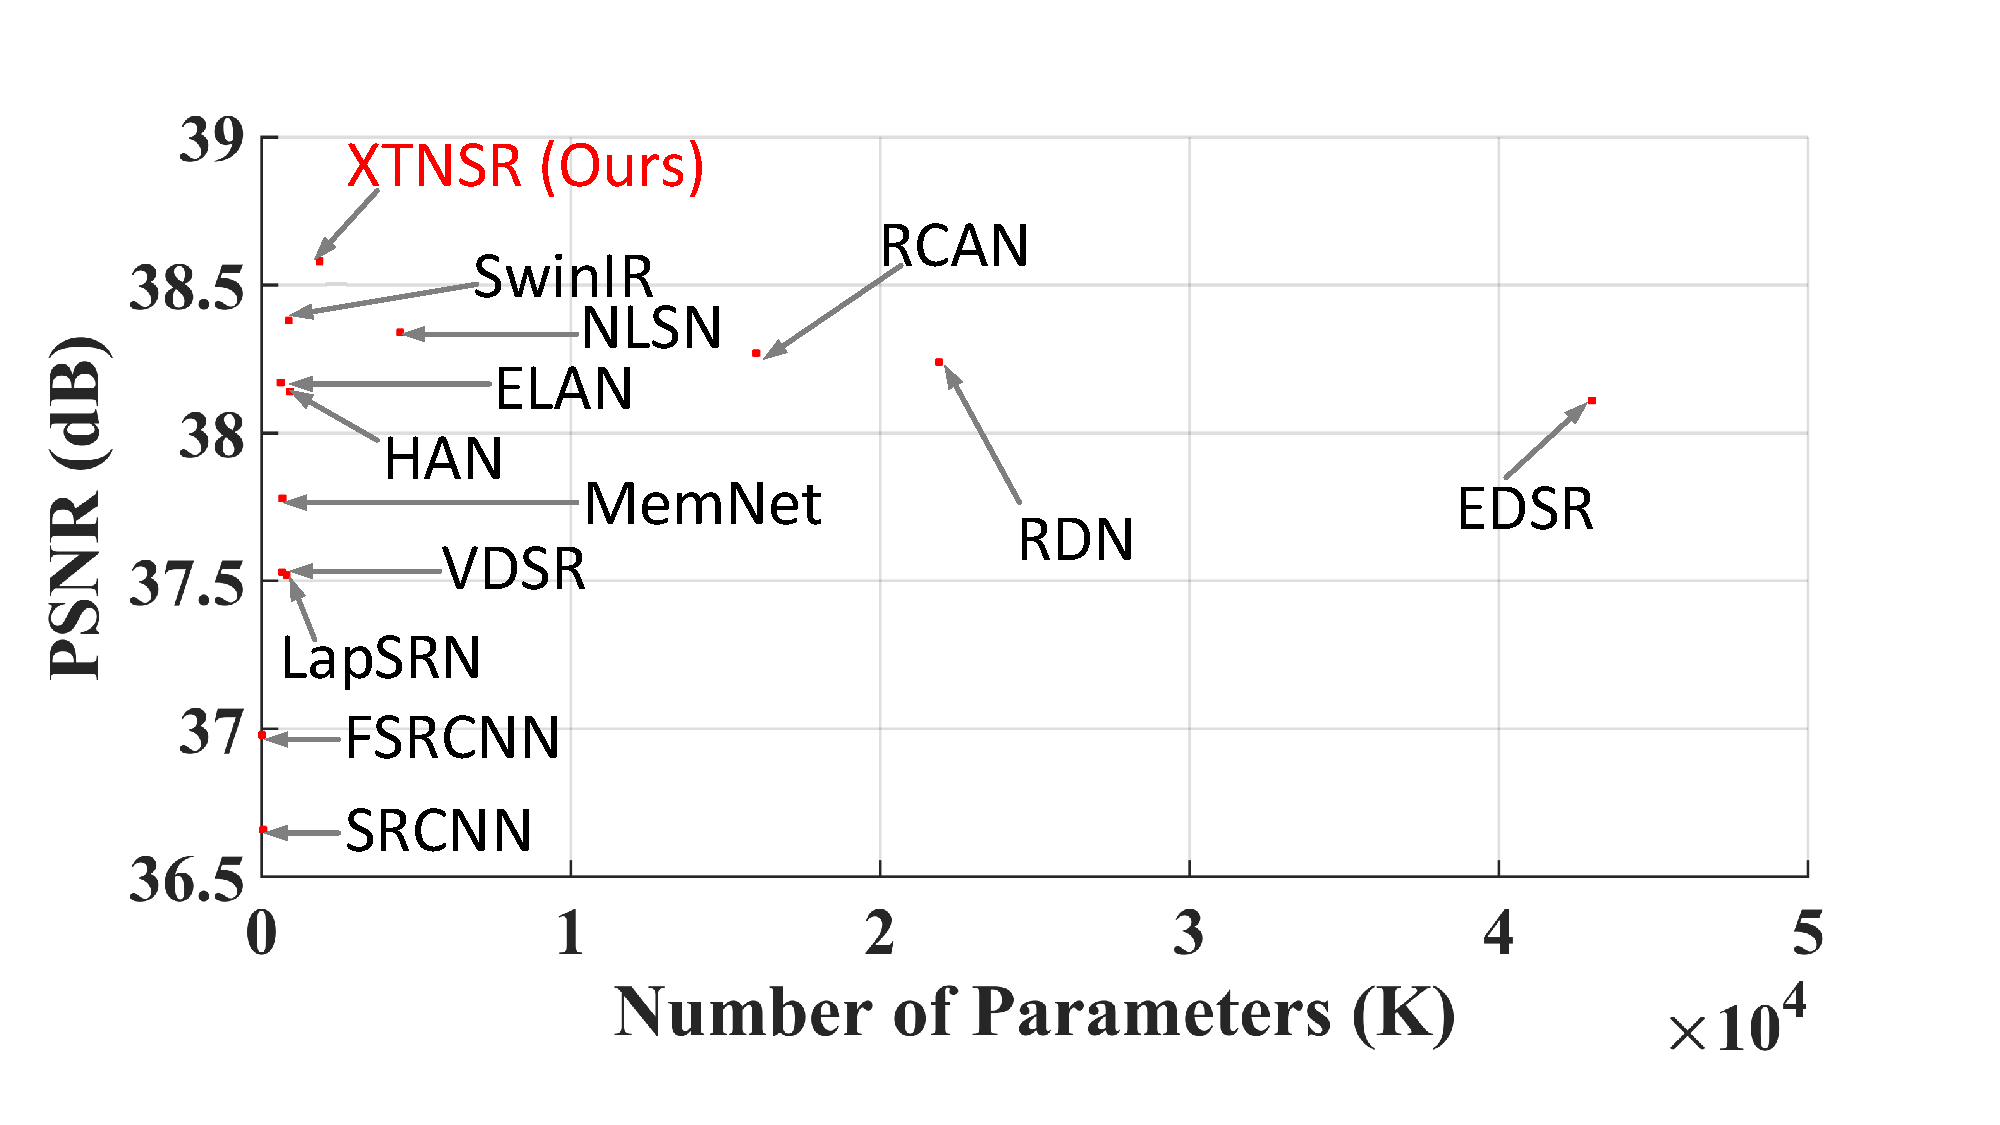
\includegraphics[width=0.5\textwidth]{6FIGURE.pdf}}
   \caption {Inspection of PSNR for model parameters on ×2 up-scaling factor using the Set5 [64] image test dataset.}
    \label{fig:6}
\end{figure}

\begin{figure}
  \centering
  \subfloat{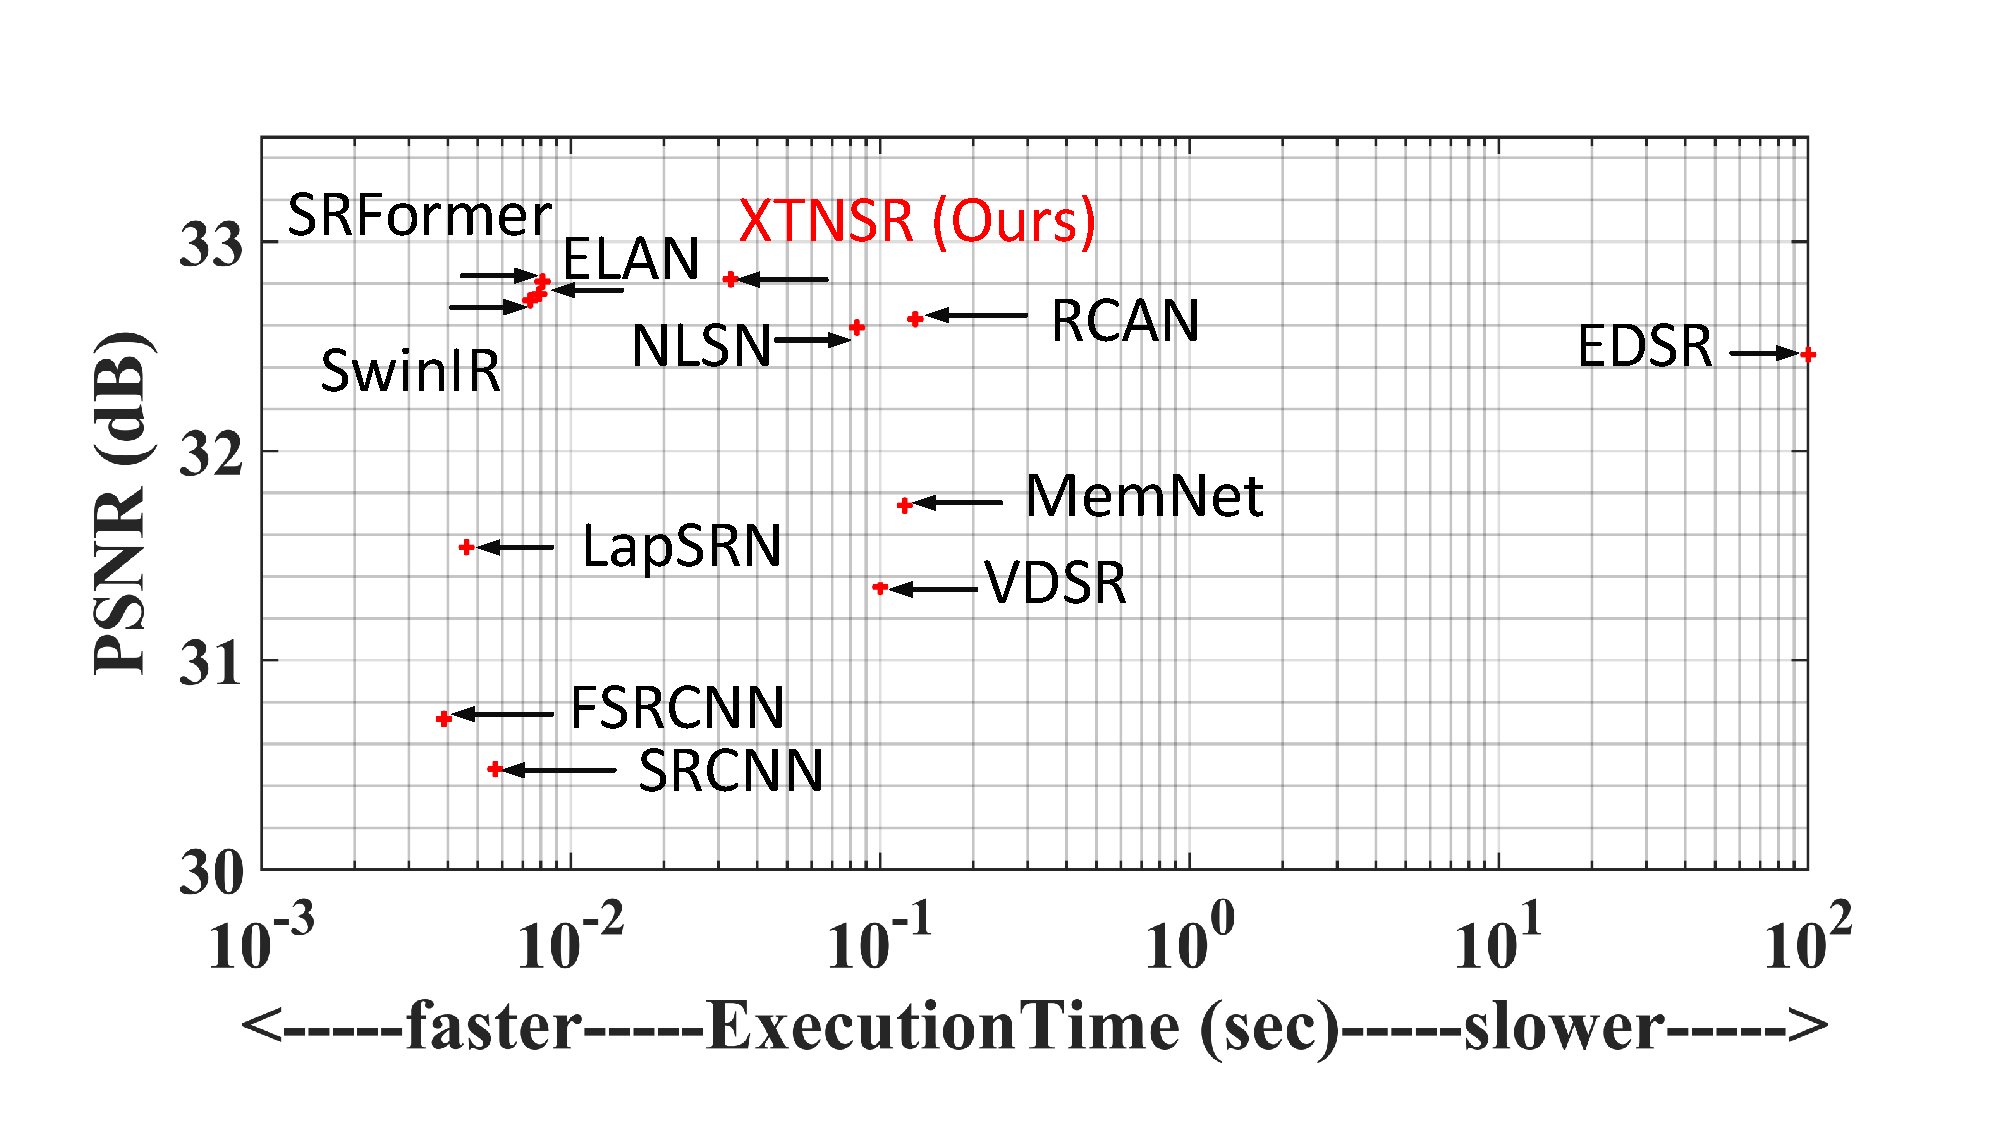
\includegraphics[width=0.5\textwidth]{7FIGURE.pdf}}
   \caption {Inspection of PSNR for execution time on ×4 up-scaling factor using the Set5 [64] image test dataset.}
    \label{fig:7}
\end{figure}

\subsection{Assessment of average PSNR and SSIM on up-scaling factors $\times$4 and $\times$8 on the Image Test Datasets}

Reporting average PSNR and SSIM scores has become standard practice in image super-resolution. This standardization facilitates a consistent and easy interpretation of the quality of super-resolved images. By calculating and reporting these metrics, researchers can demonstrate the effectiveness of their proposed approach compared to existing techniques or baselines. As seen in Figure 8 and Figure 9, our proposed XTNSR has the best average PSNR and SSIM compared to other state-of-the-art methods. The average PSNR and SSIM values are generated by taking an average of PSNR and SSIM values of all the Image SR test Dataset (i.e., Set5 [64], Set14 [65], BSD100 [66], Urban100 [67], Manga109 [68]). The average values for all the state-of-the-art models are also shown in Table 1. Figure 8 and Figure 9 represent the average values for up-scaling factors ×4 and ×8. For the up-scaling factor ×4, our suggested XTNSR achieves the most favorable outcome in comparison to RCAN [21], NLSN [23], SwinIR [26], HAN [24], and SRFormer [28]. Similarly, for the up-scaling factor $\times8$, it shows higher outcomes as compared to MemNet [15], DBPN [71], EDSR [17], RCAN [21], and HAN [24], respectively.

\begin{figure}
  \centering
  \subfloat{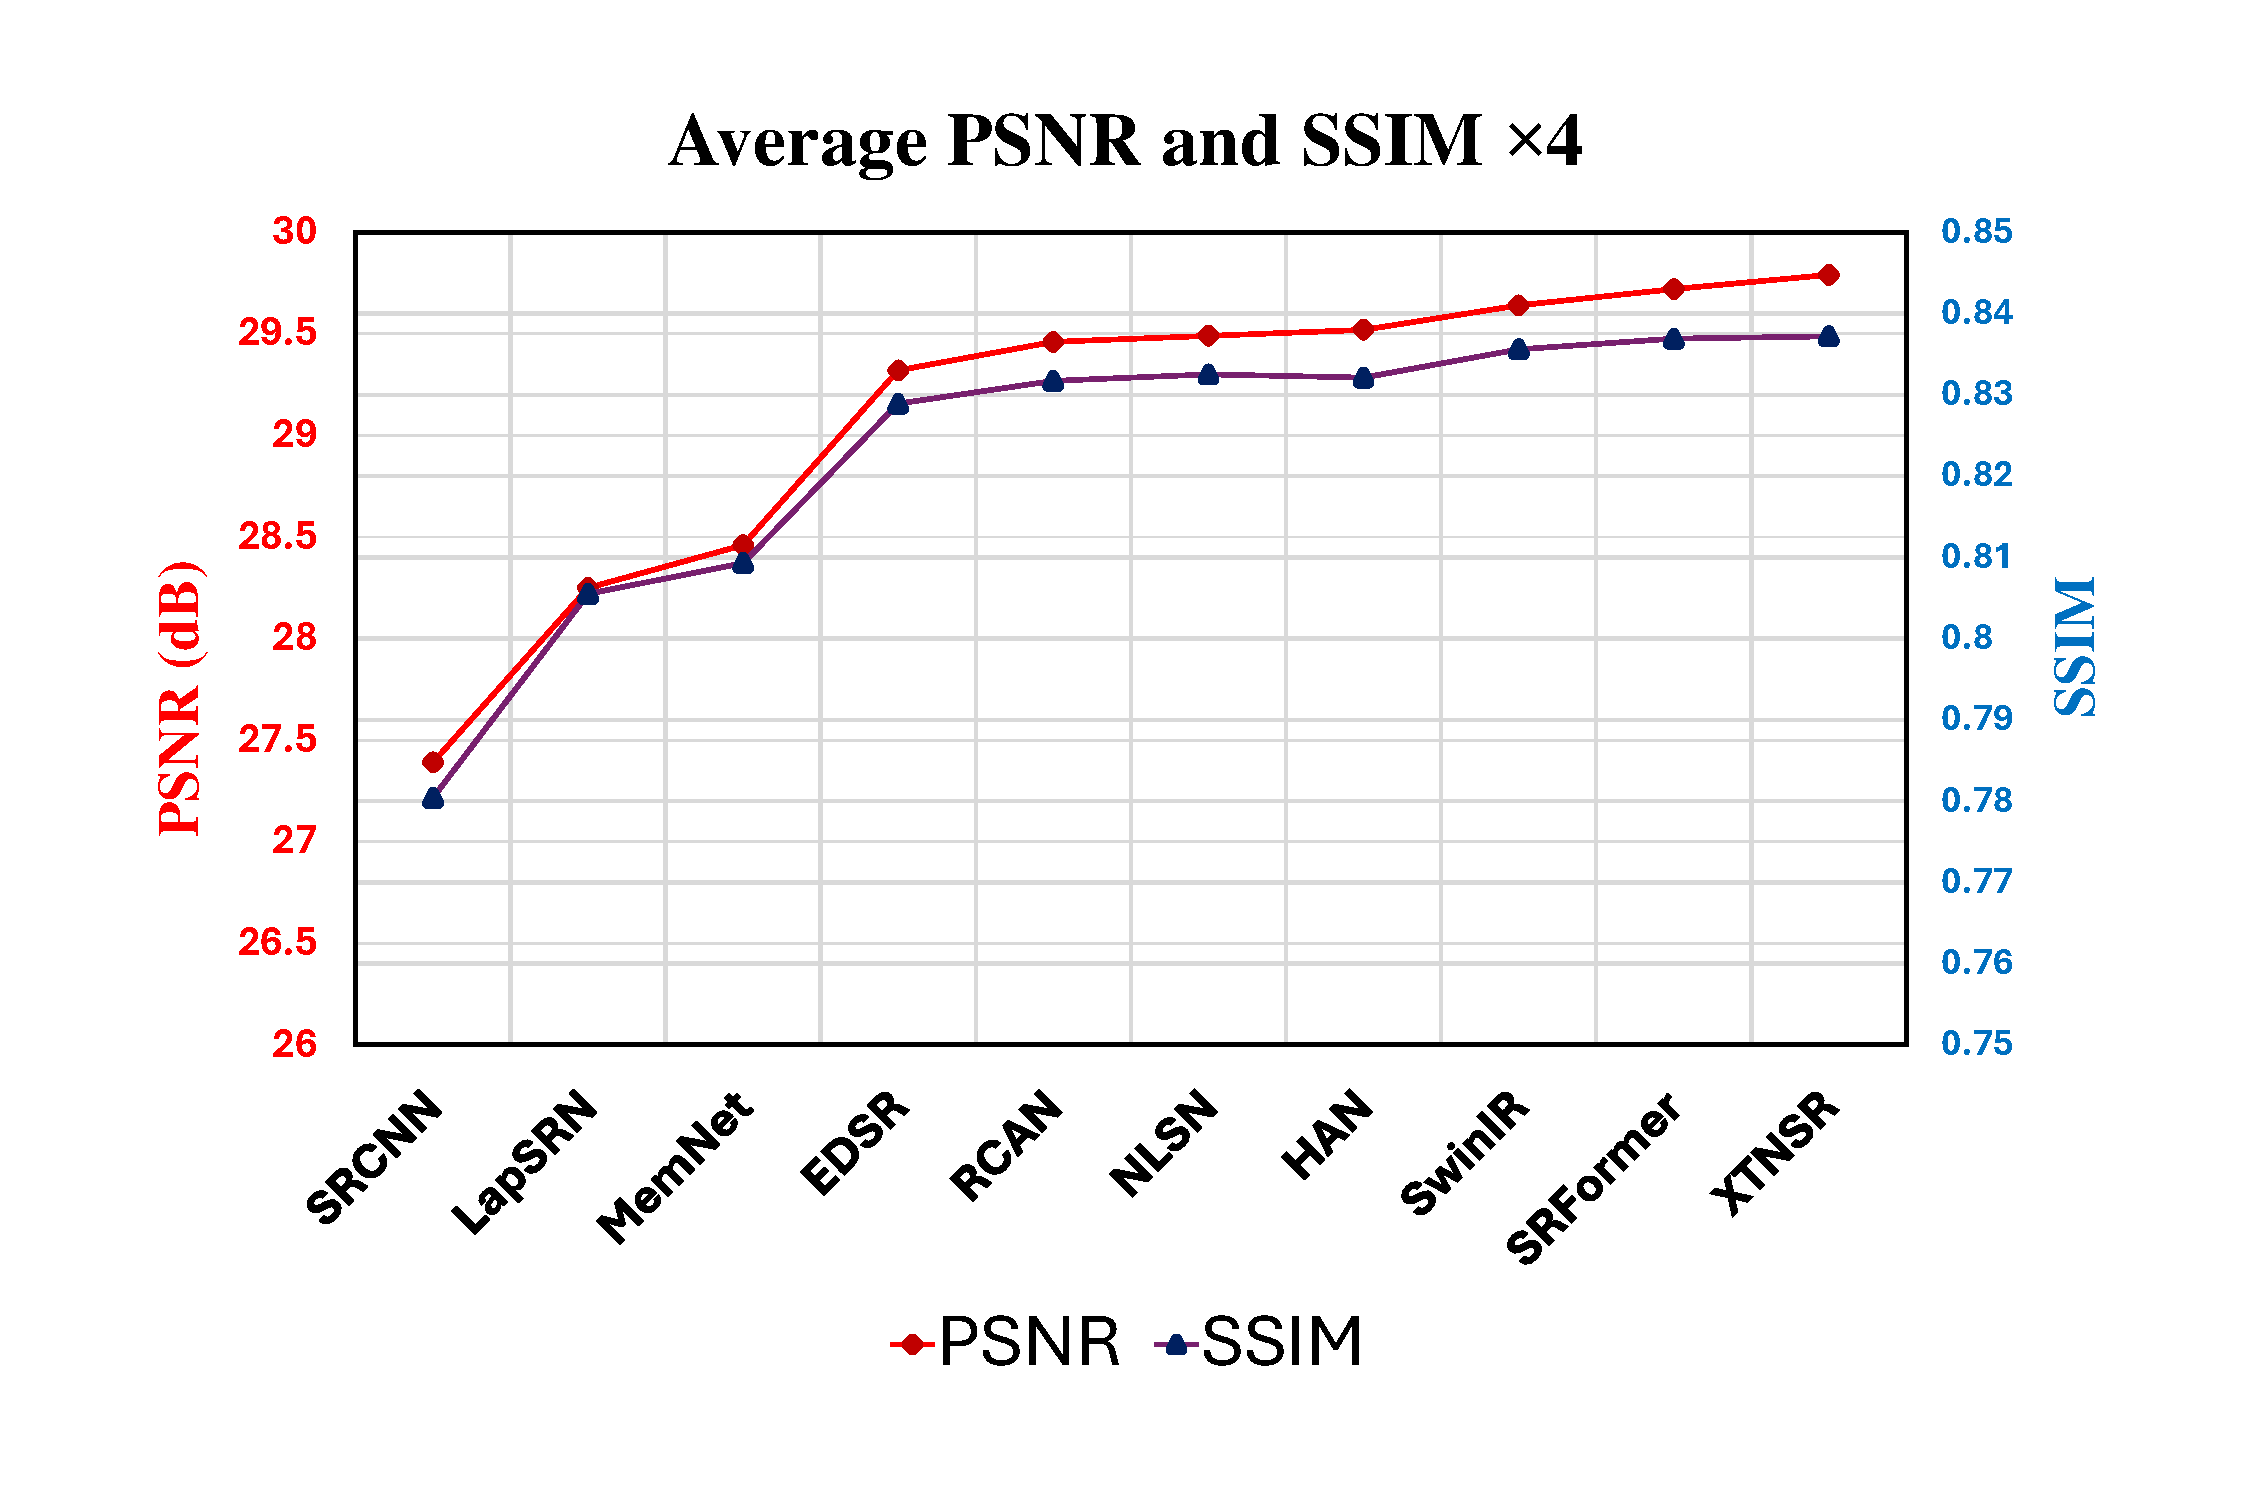
\includegraphics[width=0.5\textwidth]{8FIGURE.pdf}}
   \caption {Average PSNR and SSIM evaluation on up-scale factor ×4.}
    \label{fig:8}
\end{figure}

\begin{figure}
  \centering
  \subfloat{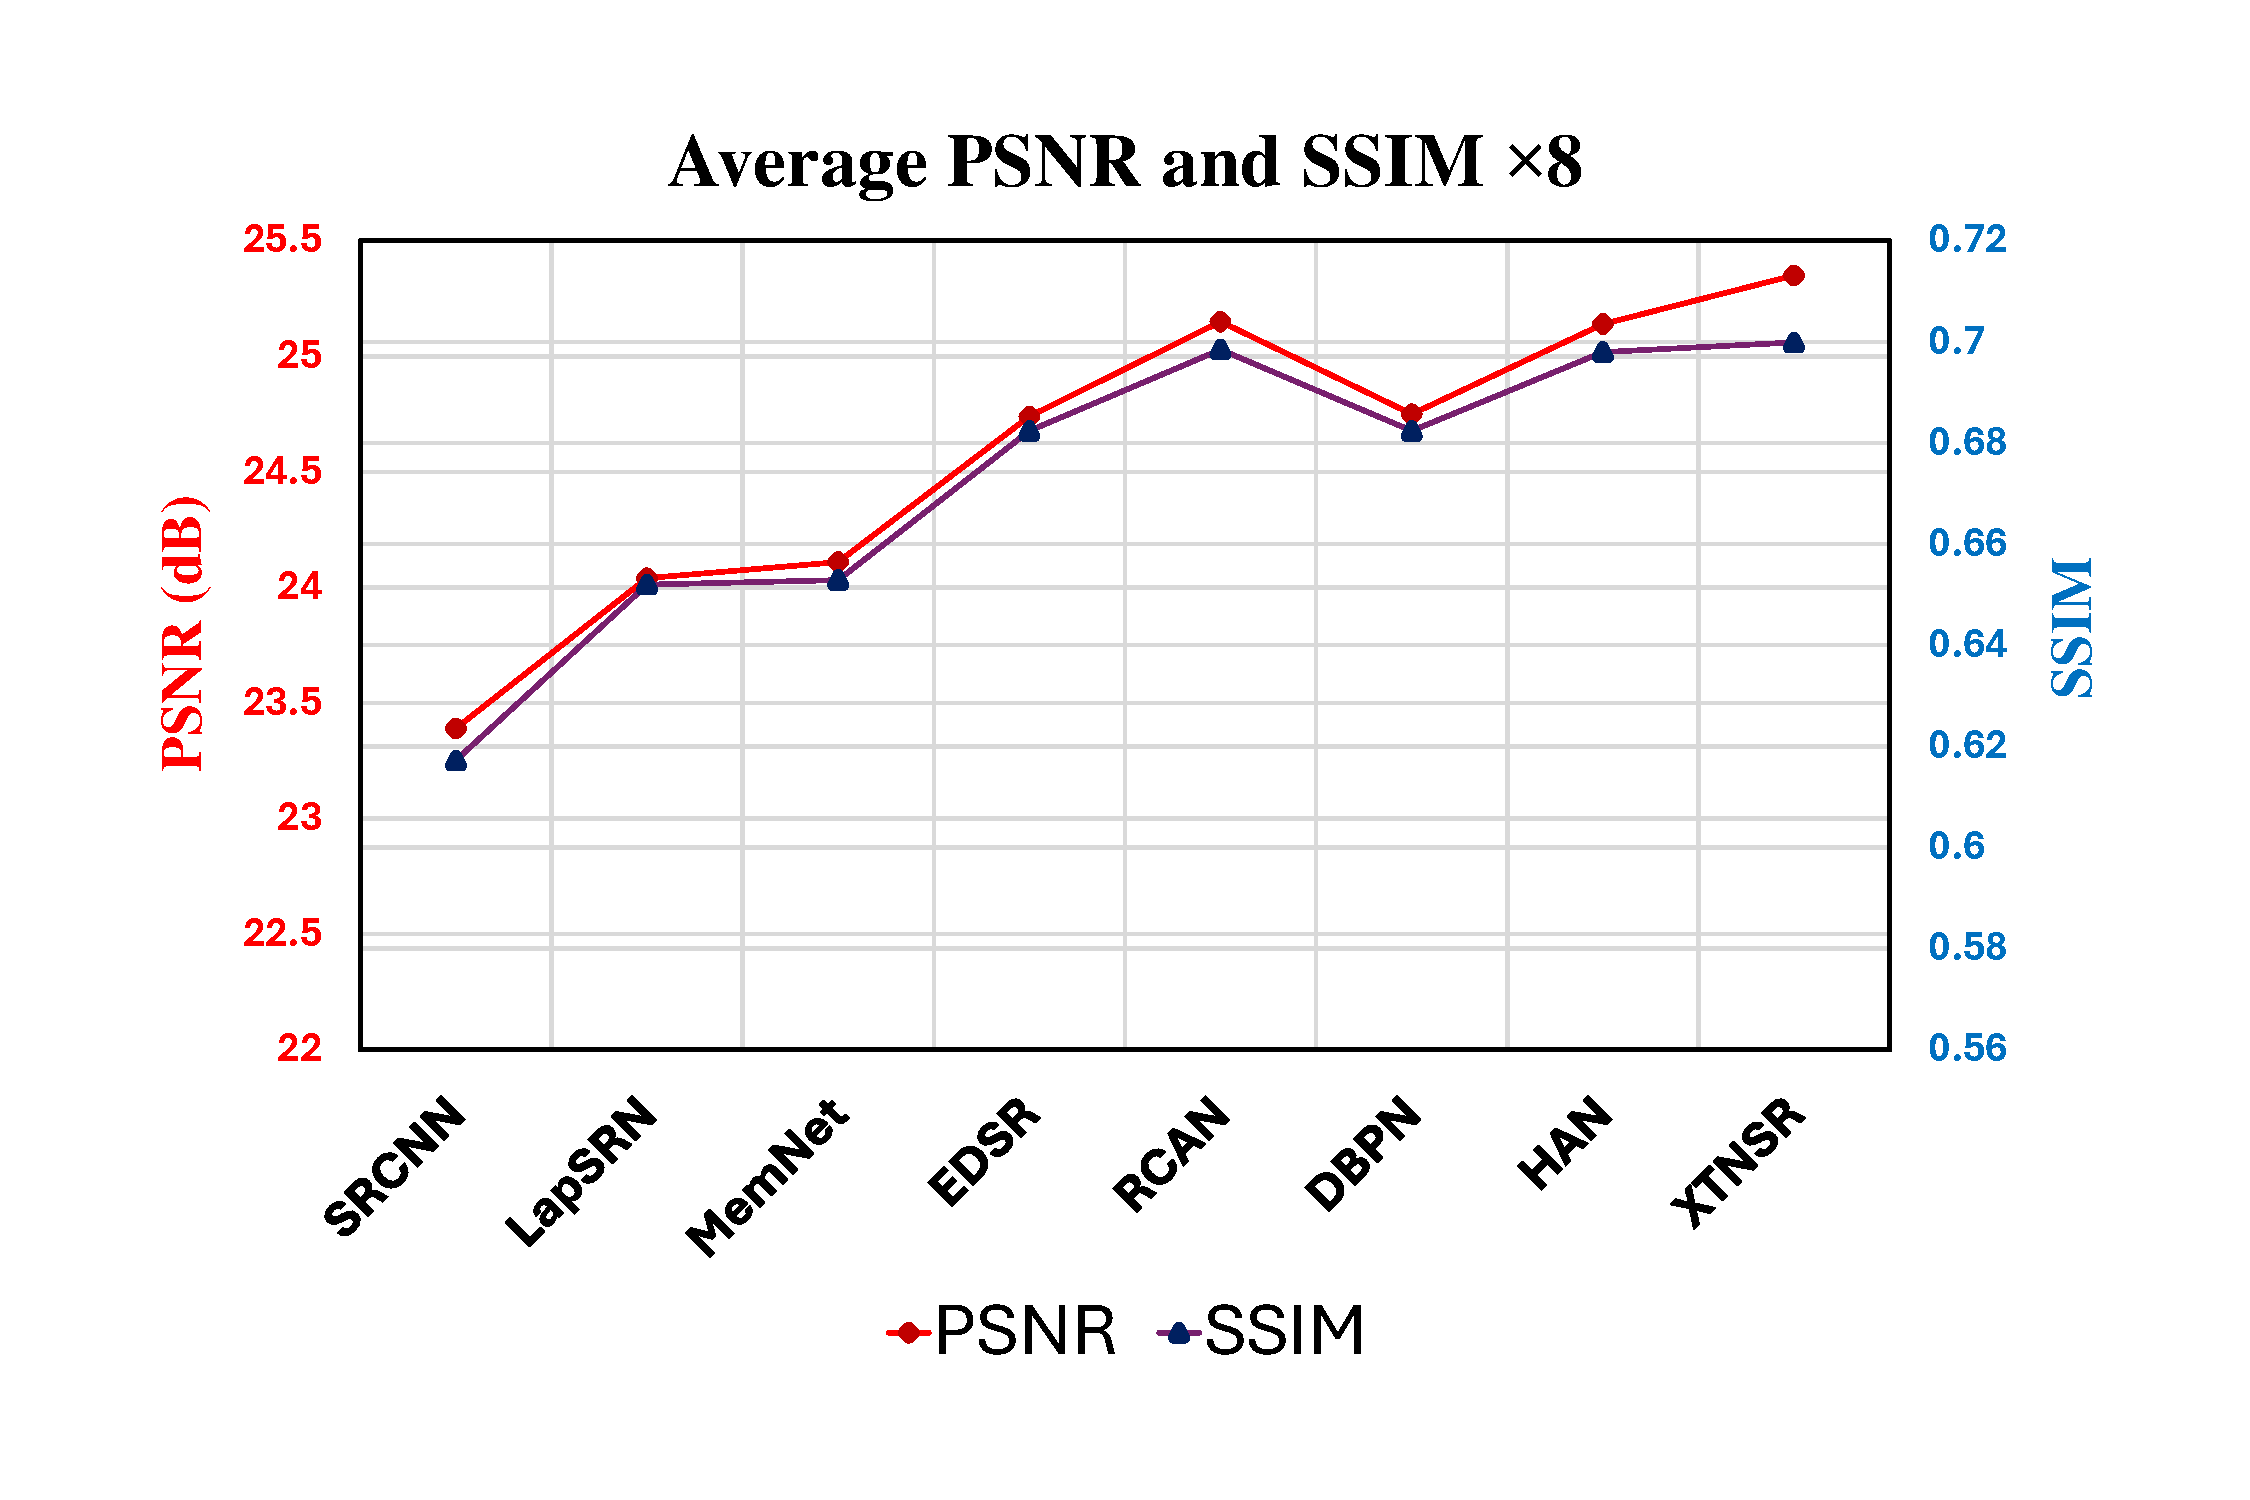
\includegraphics[width=0.5\textwidth]{9FIGURE.pdf}}
   \caption {Average PSNR and SSIM evaluation on up-scale factor ×8.}
    \label{fig:9}
\end{figure}

\subsection{Analysis with different combinations of Local Feature Window Transformer (LFWT) and Xception Blocks}

This study checked combinations of several Local Feature Window Transformers and Xception Block. Starting with using 5 LFWT and 5 Xception Blocks and trying different combinations, we observed that the best average PSNR and SSIM are obtained with the network having 6 LFWT Blocks and 4 Xception blocks. This analysis was done by training the model for 500 epochs at scale ×2. Then, the combination of 6 LFWT blocks and 4 Xception blocks was adopted in the final training of the network for 1000 epochs to obtain the best performance gains at limited computational expense. Table 2 shows that the best value of PSNR and SSIM is observed to be with 6 LFWT Blocks and 4 Xception Blocks and is highlighted in {\color{red}\textbf{red}}, and the second-best performance is observed with six LFWT Blocks and five Xception Blocks highlighted in {\color{blue}\underline{blue}}.

\begin{table*}
  \centering
  \caption{Different Combinations of LFWT and Xception Block}
  \setlength{\tabcolsep}{3 pt}
  \begin{tabular}{|c|c|c|c|c|} % Specify five columns with "c" for centered alignment
    \hline
    \textbf{Number of LFWT Blocks} & \textbf{Number of Xception Blocks} & \textbf{Average PSNR} & \textbf{Average SSIM} \\
    \hline
    5   & 5   & 37.58   & 0.9598   \\
    5   & 6   & 37.62   & 0.9602   \\
    6   & 5   & {\color{blue}\underline{37.78}}   & {\color{blue}\underline{0.9609}}   \\
    6   & 4   & {\color{red}\textbf{37.82}}   & {\color{red}\textbf{0.9611}}   \\
    4   & 6   & 37.76   & 0.9606   \\    
    4   & 4   & 37.49   & 0.9587   \\
    6   & 6   & 37.68   & 0.9604   \\
% Add more rows as needed
    \hline
  \end{tabular}
\end{table*}

\subsection{Network complexity analysis in terms of space and time}

Space complexity analysis of a deep learning model typically refers to the amount of memory or storage required by the model during training and inference. The space complexity depends on various factors, including the model architecture, parameters, and input data size. In this section, the space complexity for image data has been presented. We assess the space complexity on the Image SR text datasets with an up-scaling factor of ×2. The space complexity of our proposed XTNSR, along with HR, LR, SRCNN [8], RCAN [21], and ELAN [25], is shown in Figure 10. 

A deep learning model's time complexity can be seen in the time needed to complete each epoch during training. The model's overall complexity affects the time complexity, including the neural network's depth and width. The ability to parallelize computations across multiple devices or nodes can impact time complexity. Optimization techniques, such as model quantization or pruning, may impact training and inference time complexity. Figure 11 compares our suggested XTNSR with state-of-the-art NLSN [23] and ELAN [25] regarding time complexity. From Figure 11, it can be observed that in comparison to other methods, our proposed XTNSR network takes less time per epoch for 100 training epochs. This shows our model is also better in terms of time complexity.

\begin{figure}
  \centering
  \subfloat{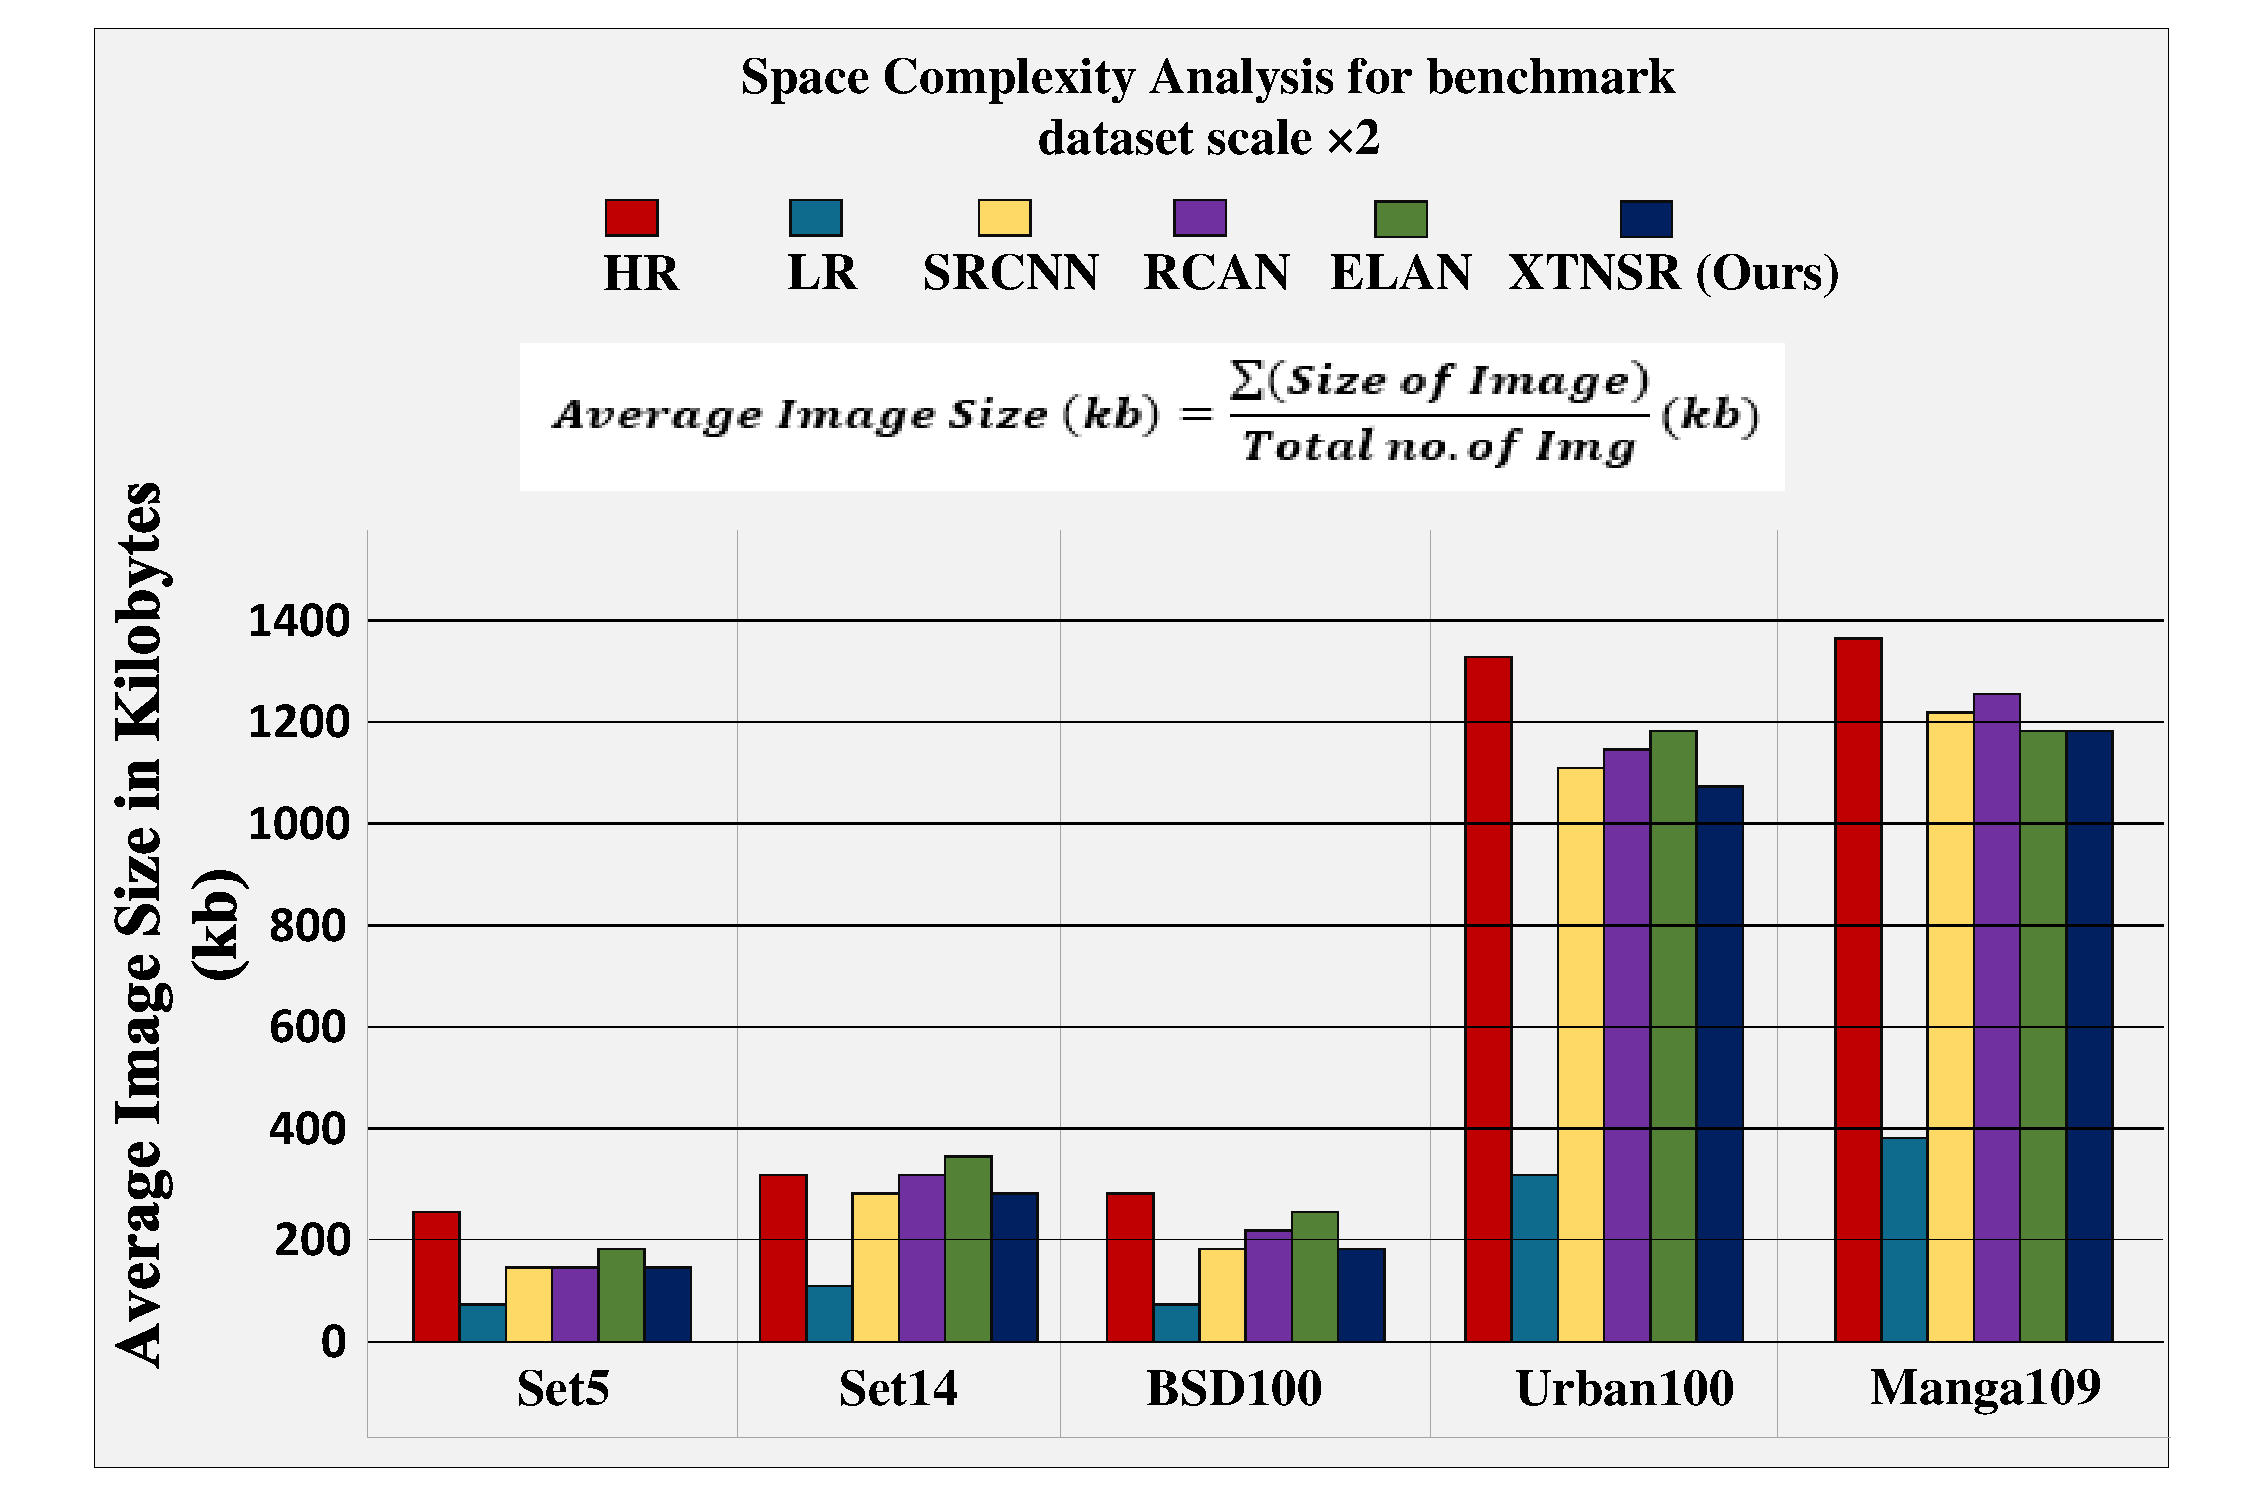
\includegraphics[width=0.5\textwidth]{10FIGURE.pdf}}
   \caption {Space Complexity assessment of network on Image SR Test Data Sets on up-scaling factor  ×2.}
    \label{fig:10}
\end{figure}

\begin{figure}
  \centering
  \subfloat{\includegraphics[width=0.5\textwidth]{11FIGURE.png}}
   \caption {Evaluation of run time against PSNR on Set5 [64] for up-scale factor ×4.}
    \label{fig:11}
\end{figure}

\subsection{Perceptual Quality Comparison}
The perceived accuracy at up-scaling factors ×4 and ×8 for image SR testing datasets, such as Set5 [64], Set14 [65], BSD100 [66], Urban100 [67], and Manga109 [68], is presented in Figure 12, Figure 13, Figure 14, Figure 15, Figure 16, Figure 17, Figure 18, and Figure 19. While improving an image for an enlargement factor of ×8 is challenging, our suggested XTNSR reconstructs the finer details in an image, efficiently removes general artifacts, and provides realistic visual results by reducing over-smoothing. 
Some examples of the generated high-quality images from each test dataset at scale factor ×4 and ×8 have been presented in Figure 12, Figure 13, Figure 14, Figure 15, Figure 16, Figure 17, Figure 18, and Figure 19. On up-scaling factor ×4, for Set14 [65], we used the Barbara image, and for the BSD100 [66] dataset, we used the Img\_78004 image. For the Urban100 [67] dataset, we used Img\_004, and for the Manga109 [68] dataset, we used GakuenNoise Image. For these images, we have shown the comparison of our proposed method with eight existing state-of-the-art methods, including Bicubic, MSRN [69], EDSR [17], AWSRN [70], RCAN [21], NLSN [23], SwinIR [26] and SRFormer [28].

\begin{figure*}
  \centering
  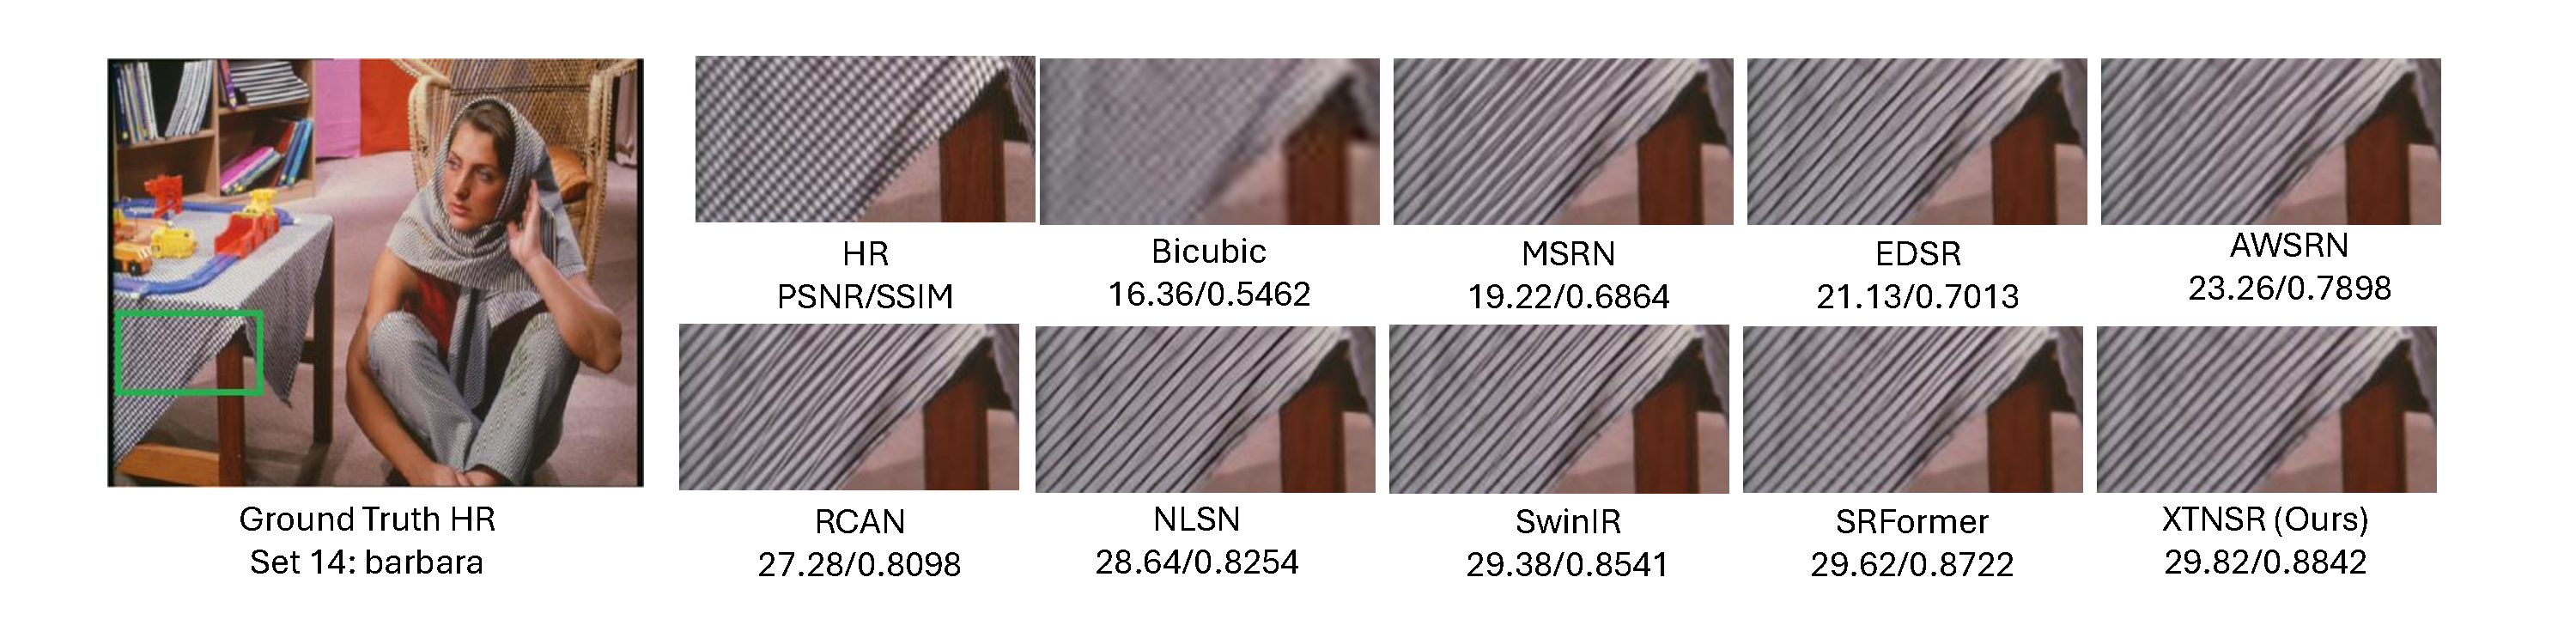
\includegraphics[width=\linewidth]{12FIGURE.pdf}
   \caption {Barbara's image from the Set14 [65] dataset perceptual improvement on a ×4 up-scaling factor.}
    \label{fig:12}
\end{figure*}

\begin{figure*}
  \centering
  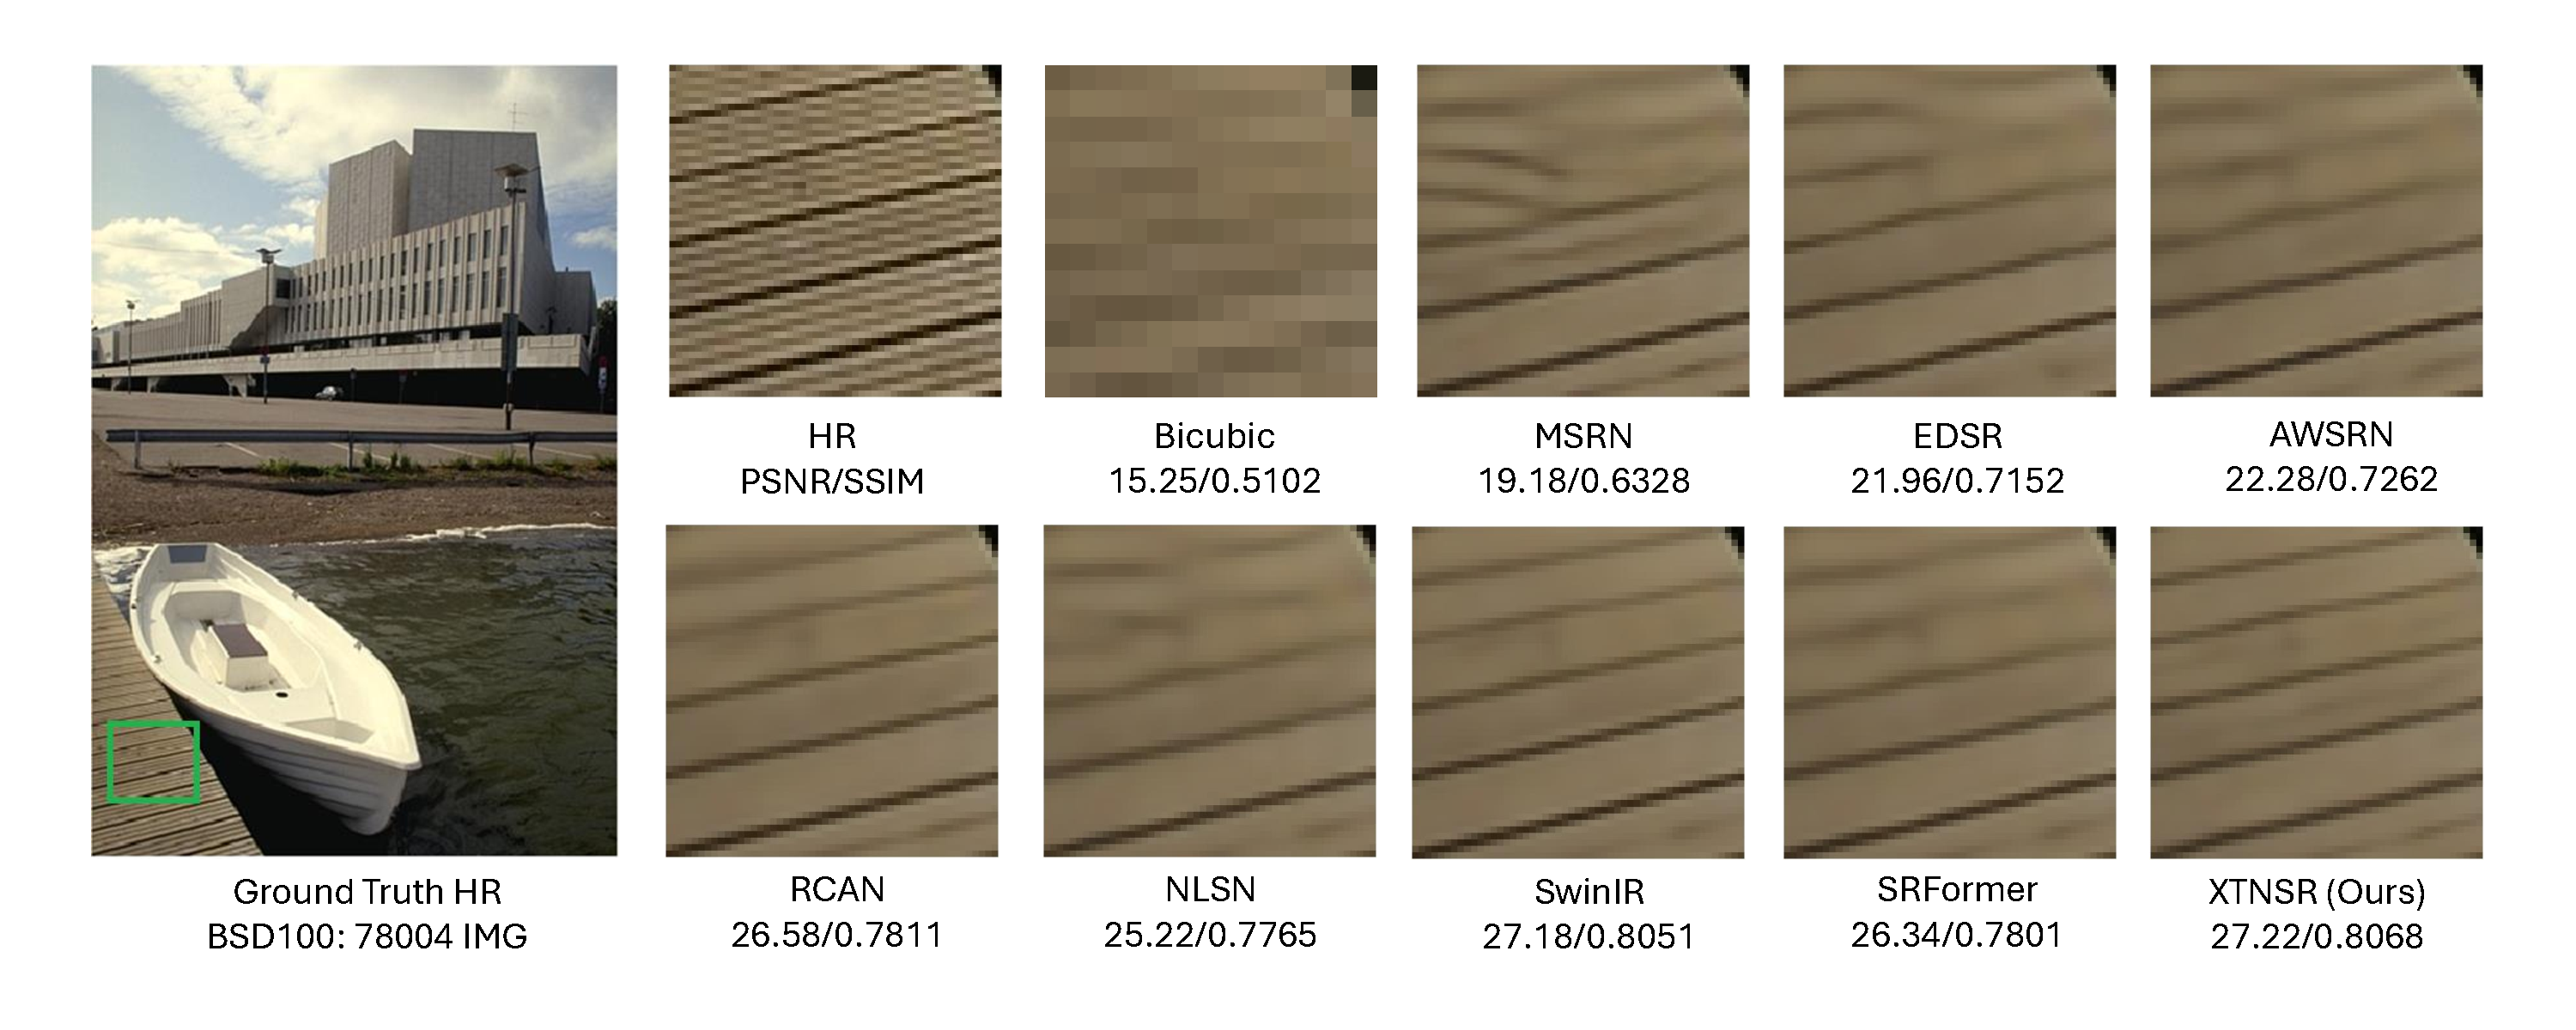
\includegraphics[width=\linewidth]{13FIGURE.pdf}
   \caption {Img\_78004 image from the BSD100 [66] dataset perceptual improvement on a ×4 up-scaling factor.}
    \label{fig:13}
\end{figure*}

\begin{figure*}
  \centering
  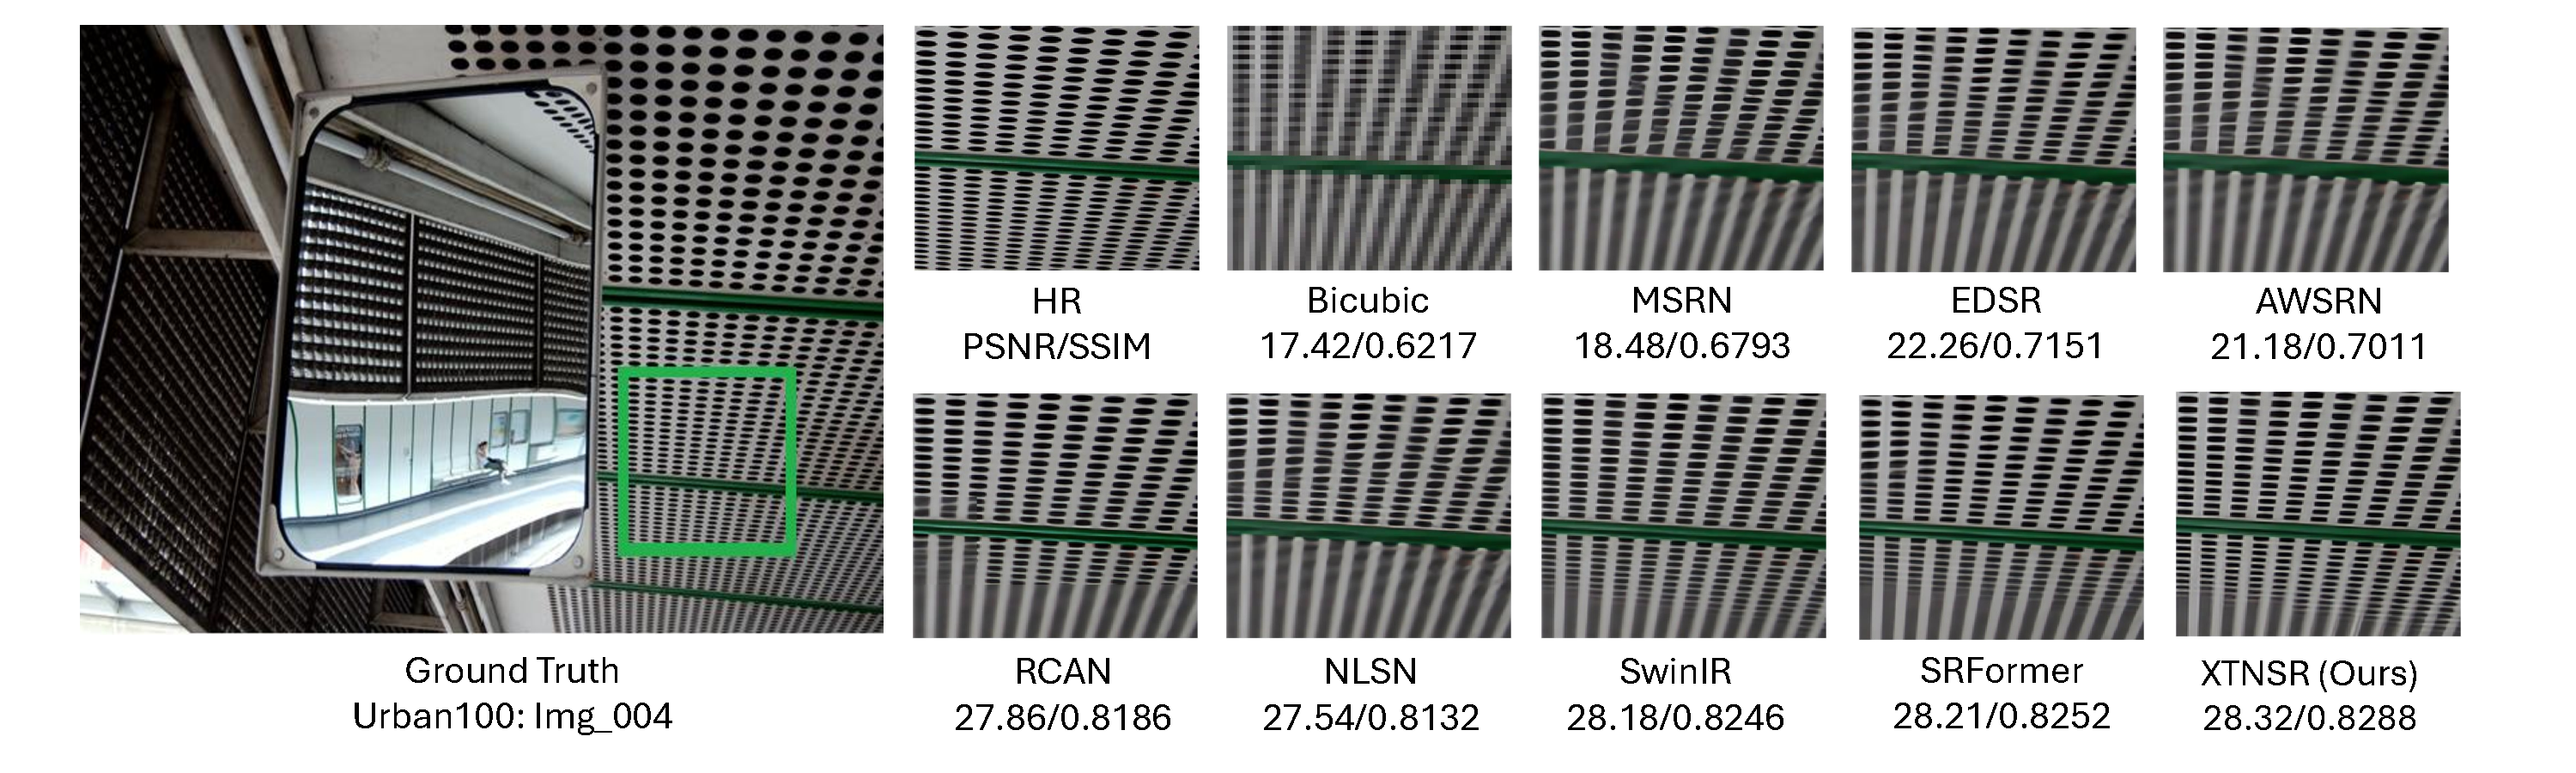
\includegraphics[width=\linewidth]{14FIGURE.pdf}
   \caption {Img\_004 image from the Urban100 [67] dataset perceptual improvement on a ×4 up-scaling factor.}
    \label{fig:14}
\end{figure*}

\begin{figure*}
  \centering
  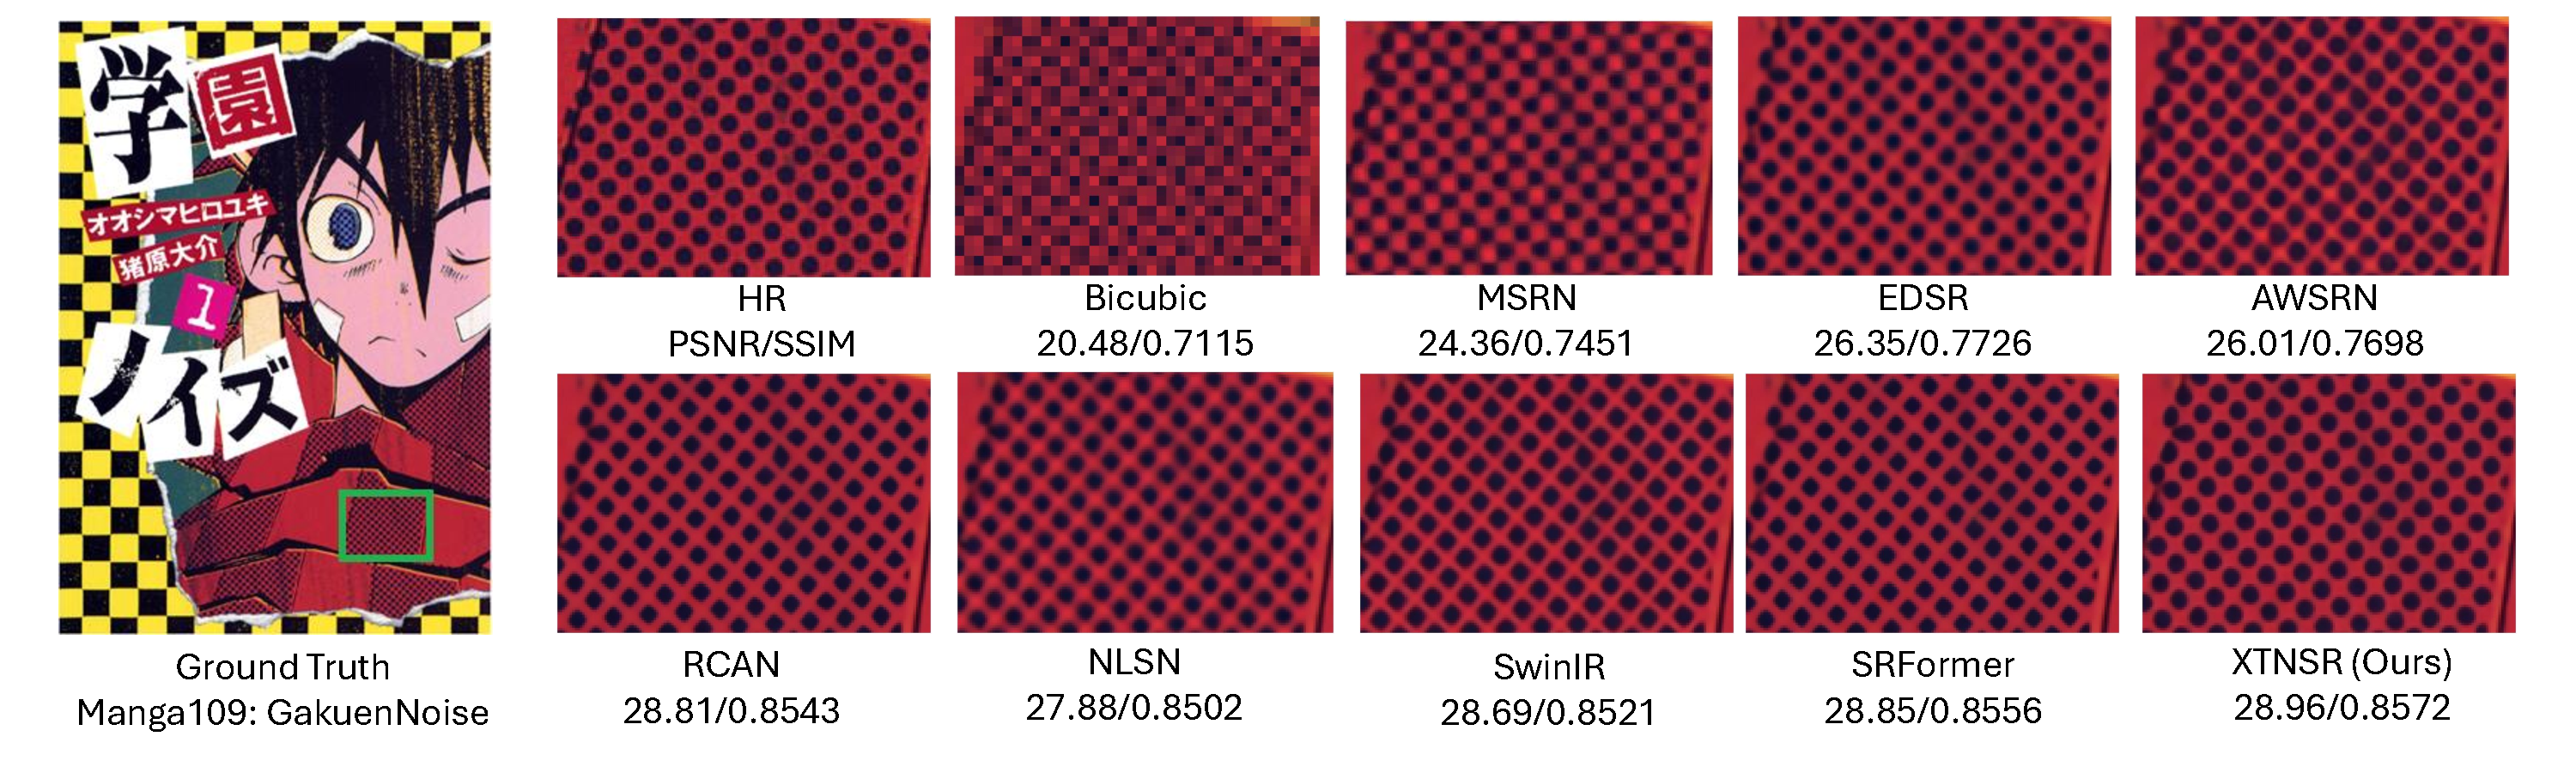
\includegraphics[width=\linewidth]{15FIGURE.pdf}
   \caption {GakuenNoise image from the Manga109 [68] dataset perceptual improvement on a ×4 up-scaling factor.}
    \label{fig:15}
\end{figure*}

\begin{figure*}
  \centering
  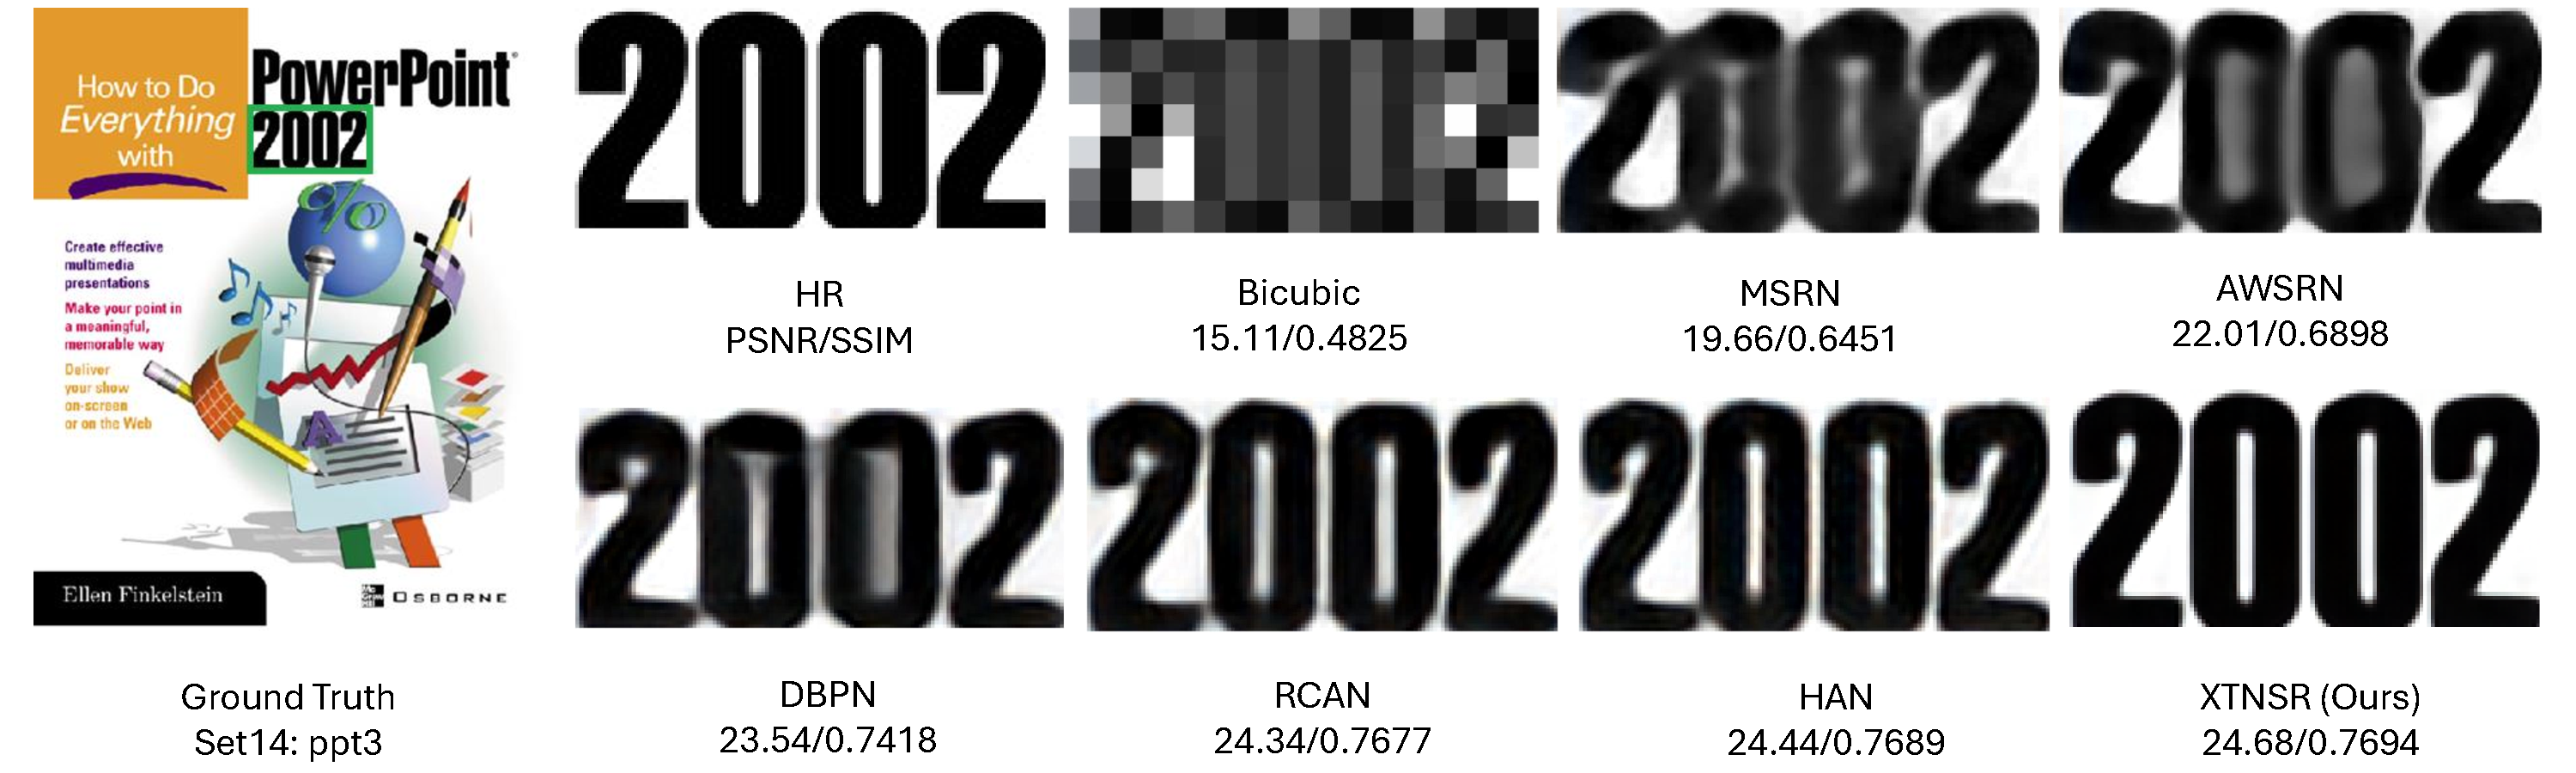
\includegraphics[width=\linewidth]{16FIGURE.pdf}
   \caption {ppt3 image from the Set14 [65] dataset perceptual improvement on a ×8  up-scaling factor.}
    \label{fig:16}
\end{figure*}

\begin{figure*}
  \centering
  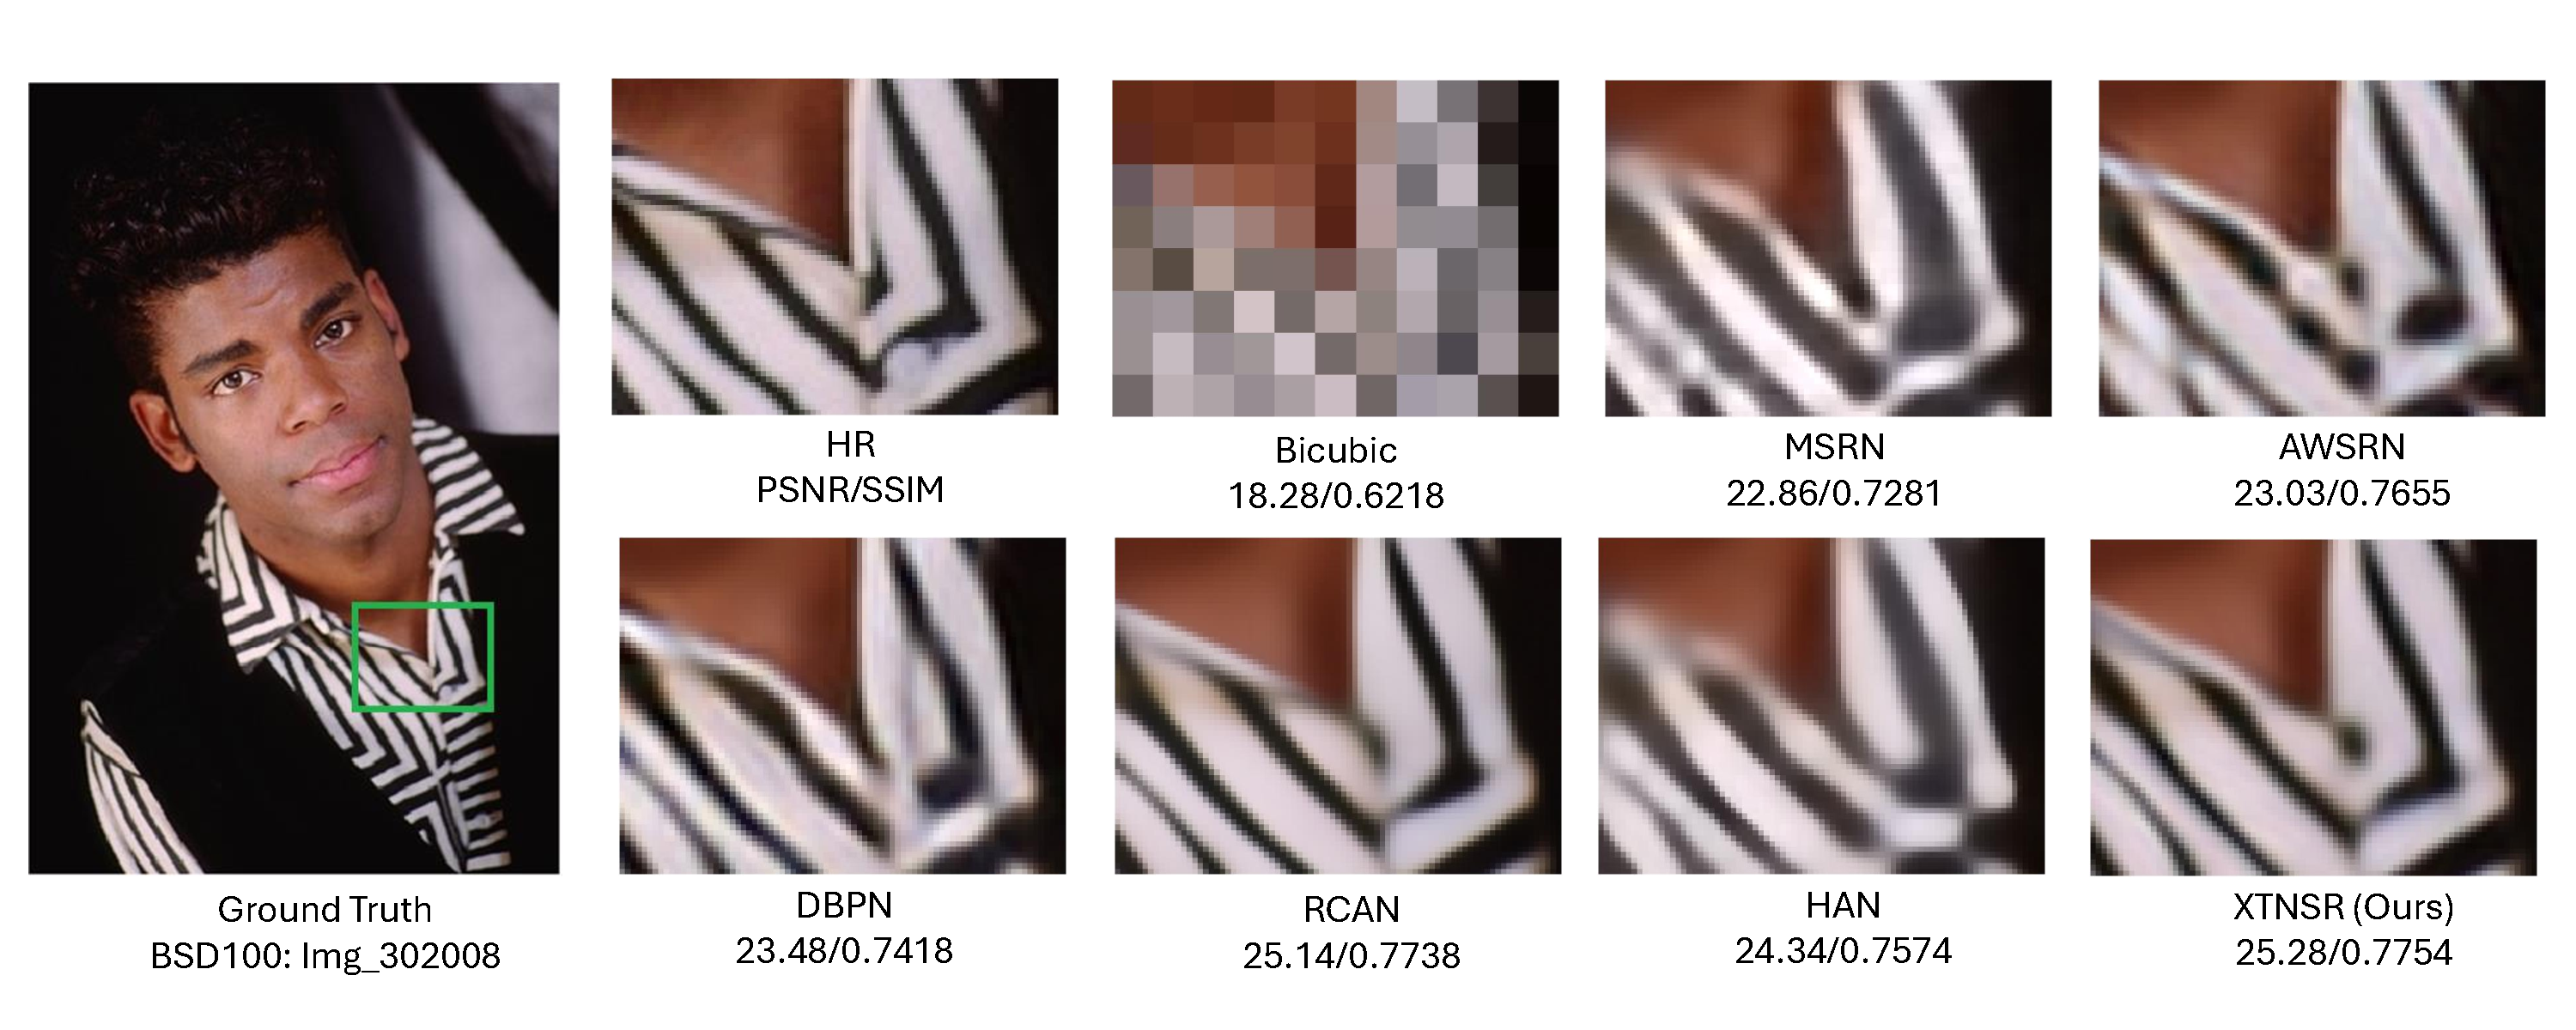
\includegraphics[width=\linewidth]{17FIGURE.pdf}
   \caption {Img\_302008 image from the BSD100 [66] dataset perceptual improvement on a ×8 up-scaling factor.}
    \label{fig:17}
\end{figure*}

\begin{figure*}
  \centering
  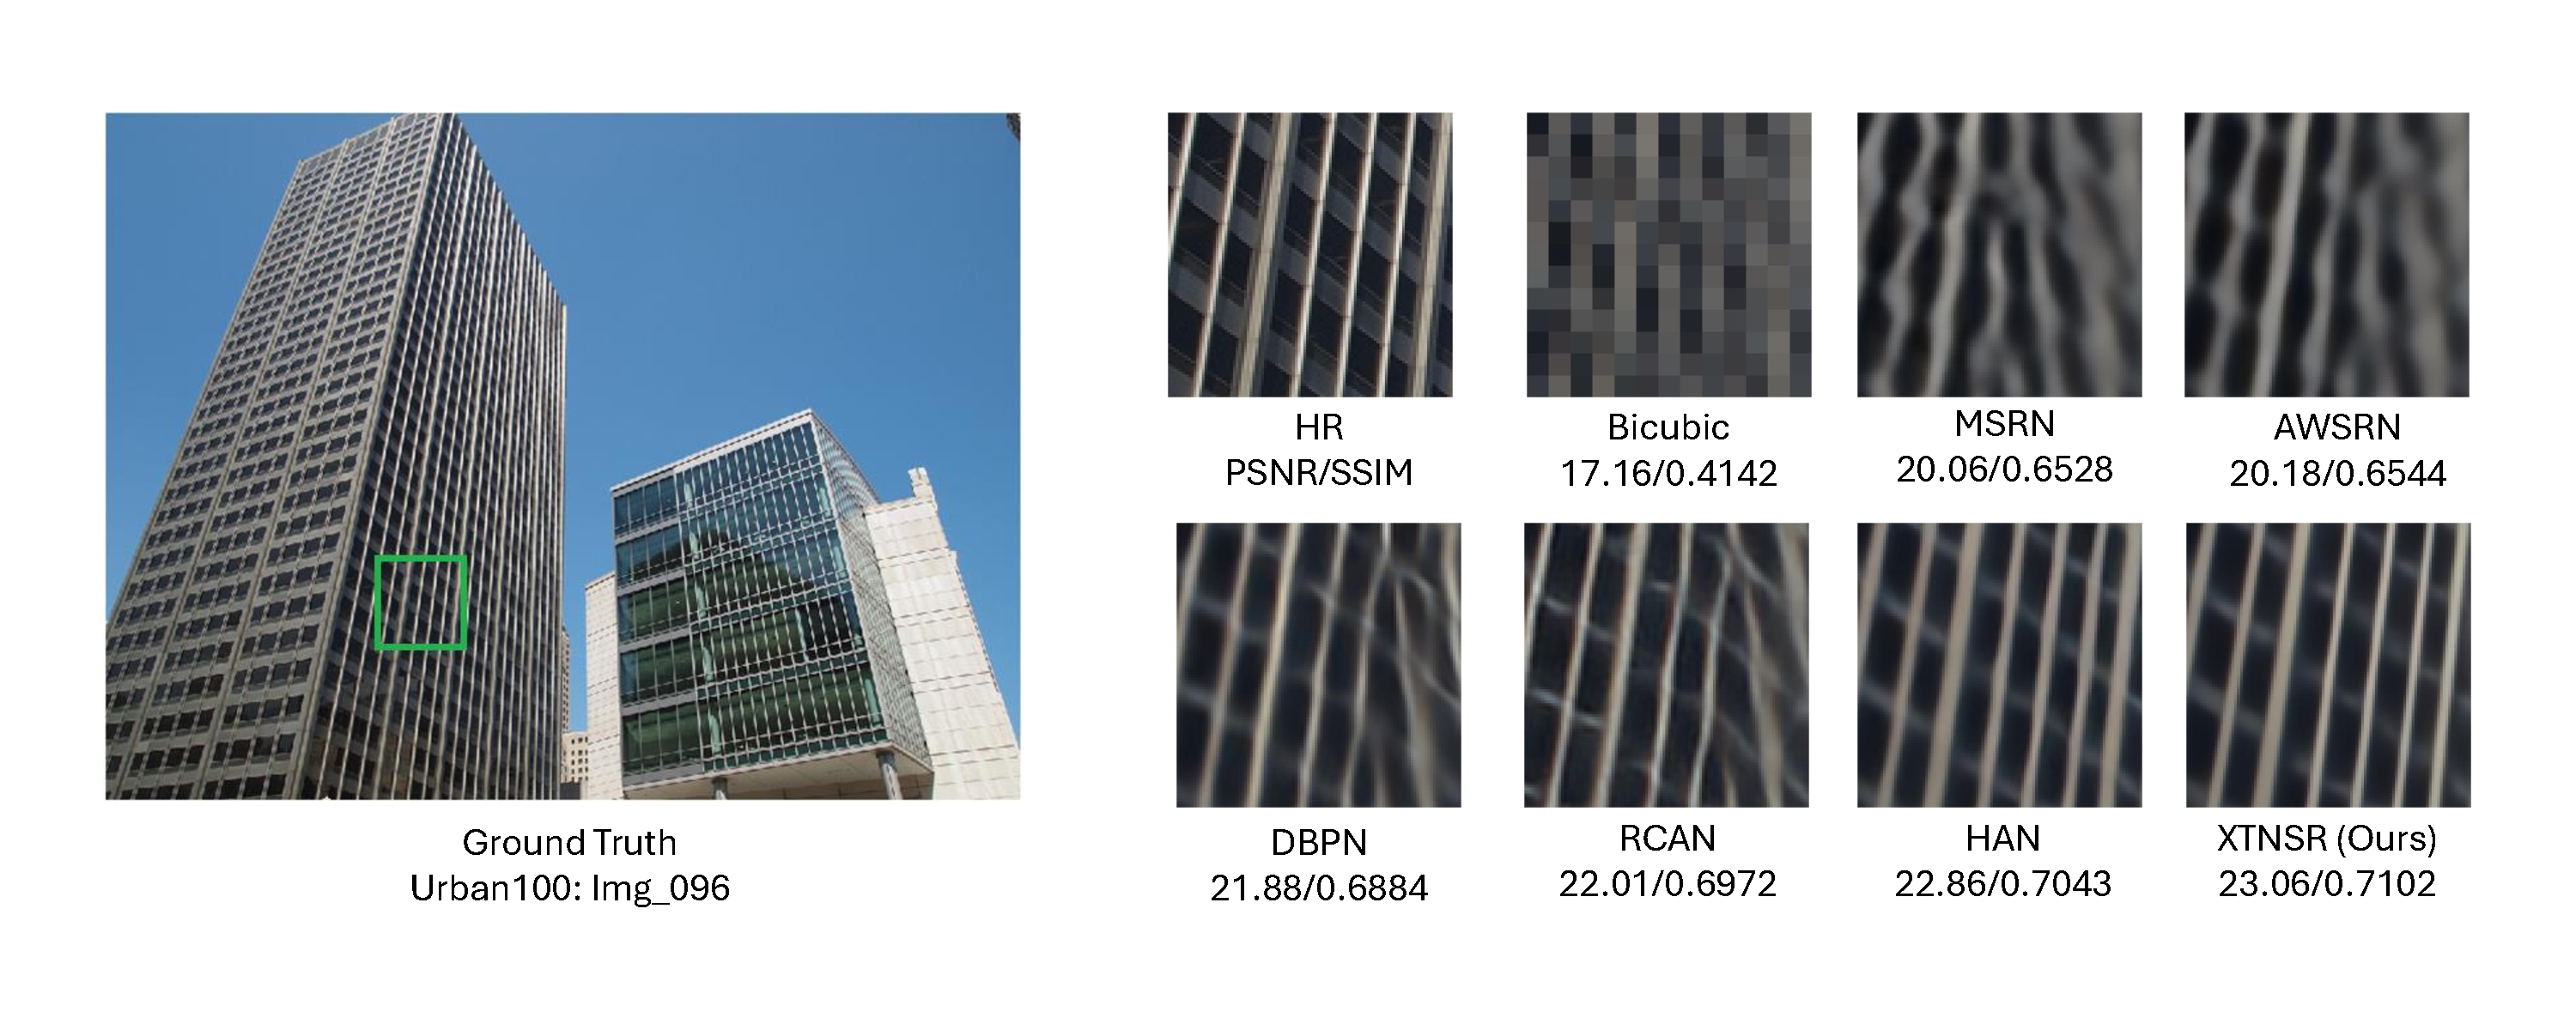
\includegraphics[width=\linewidth]{18FIGURE.pdf}
   \caption {Img\_096 image from the Urban100 [67] dataset perceptual improvement on a ×8 up-scaling factor.}
    \label{fig:18}
\end{figure*}

\begin{figure*}
  \centering
  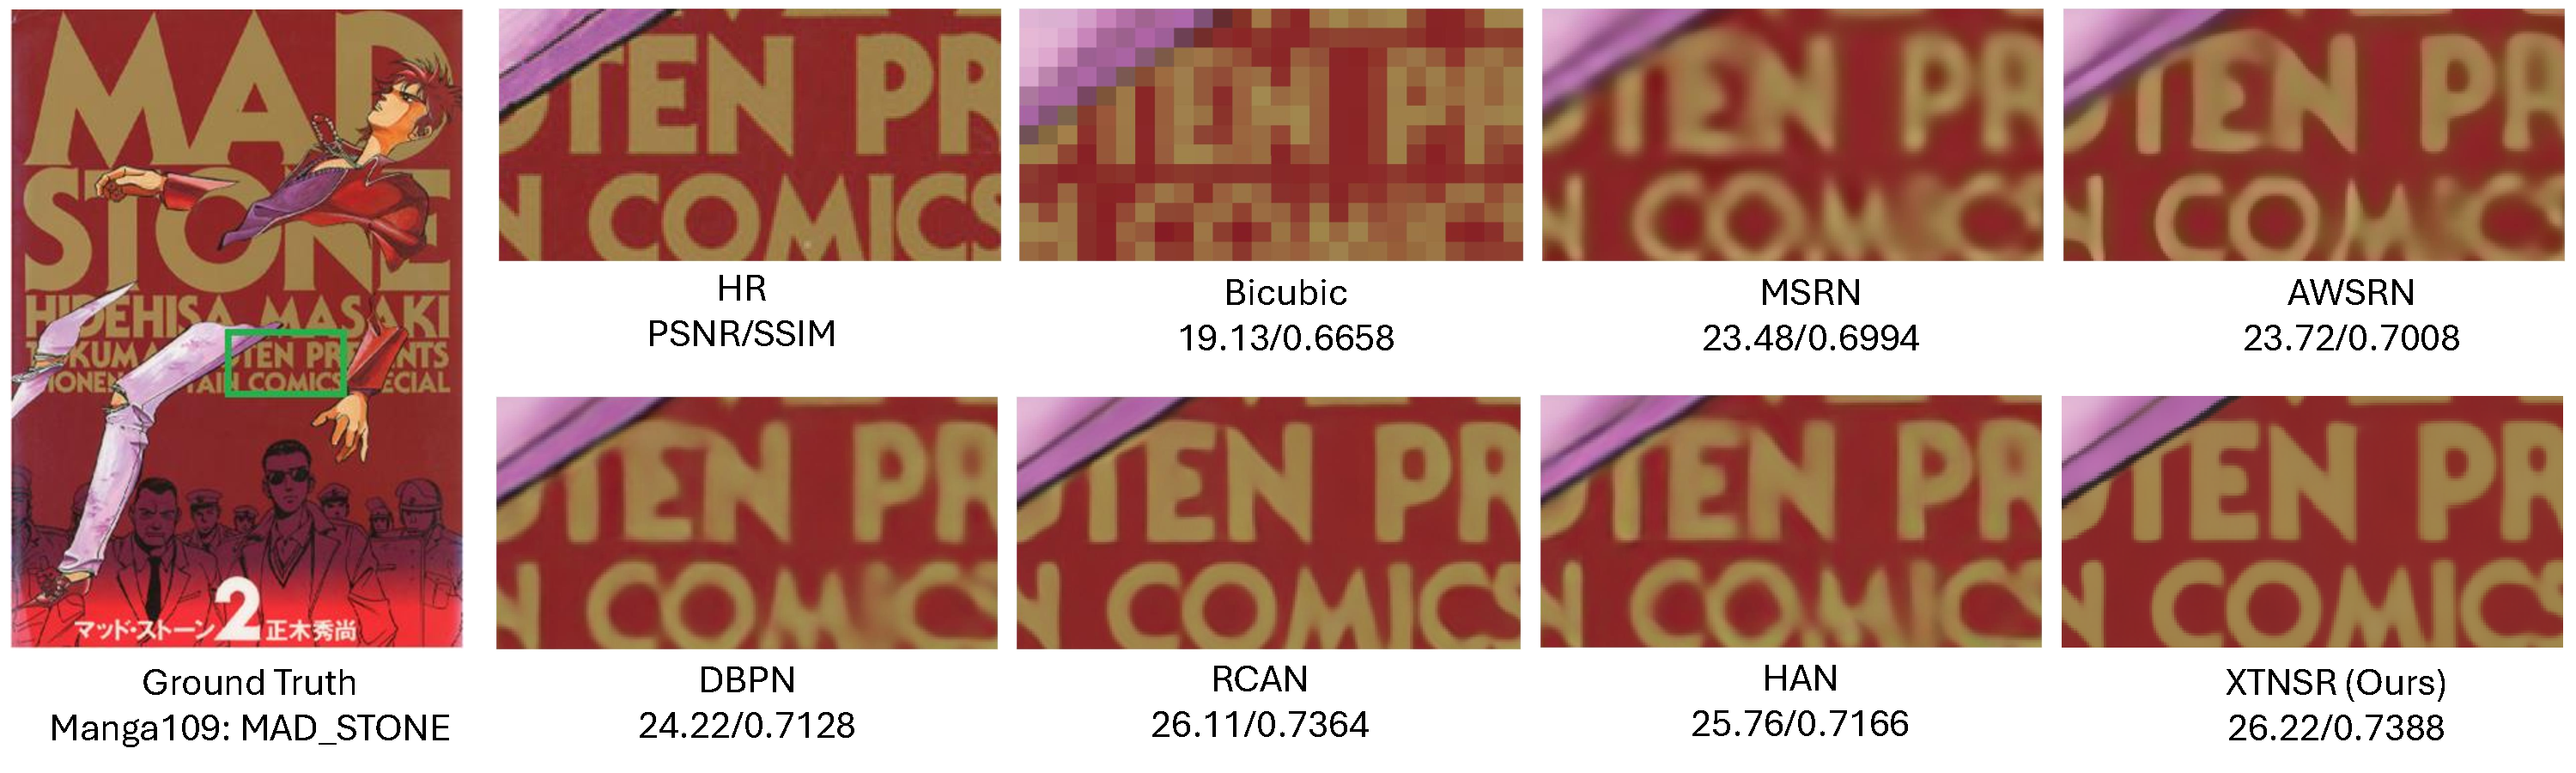
\includegraphics[width=\linewidth]{19FIGURE.pdf}
   \caption {MAD\_STONE image from the Manga109 [68] dataset perceptual improvement on a ×8 up-scaling factor.}
    \label{fig:19}
\end{figure*}

\subsection{Ablation assessment}

This section demonstrates controlled experimentation by changing algorithm hyperparameters, significantly affecting the model's performance in the ablation assessment section. The model comprises 6 Local Feature Window Transformer (LFWT) Blocks, 4 Xception Blocks, and 1 Multi-layer Feature Fusion Block. Controlled experiments have been performed on each block to determine their effect on the overall performance of the network.

Three types of ablation assessment have been performed on the model: (1) Ablation study for FLOPs versus PSNR, (2) Ablation study for changing the window size of the Local Feature Window Transformer Block, (3) Ablation study using traditional denoising methods, (4) Ablation study by changing activation functions to ReLU, PReLU, and CReLU in the Xception Block, (5) Ablation study by changing non-linearity in the Multi-Layer Feature Fusion (MLFF) Block,

\subsubsection{Ablation study for FLOPS v/s PSNR}

A study comparing PSNR (Peak Signal-to-Noise Ratio) against FLOPs (Floating Point Operations) in ISR systematically analyzes the trade-off between computational complexity and reconstruction quality. Using ten state-of-the-art image SR methods, we compared the computational cost of floating-point operations per second (FLOPs) versus PSNR for Set 5 [64] on scale factor ×4 shown in Figure 20. Figure 20 shows that, compared to SRFormer and ELAN, our suggested (XTNSR) method has fewer FLOPs. 

\begin{figure}
  \centering
  \subfloat{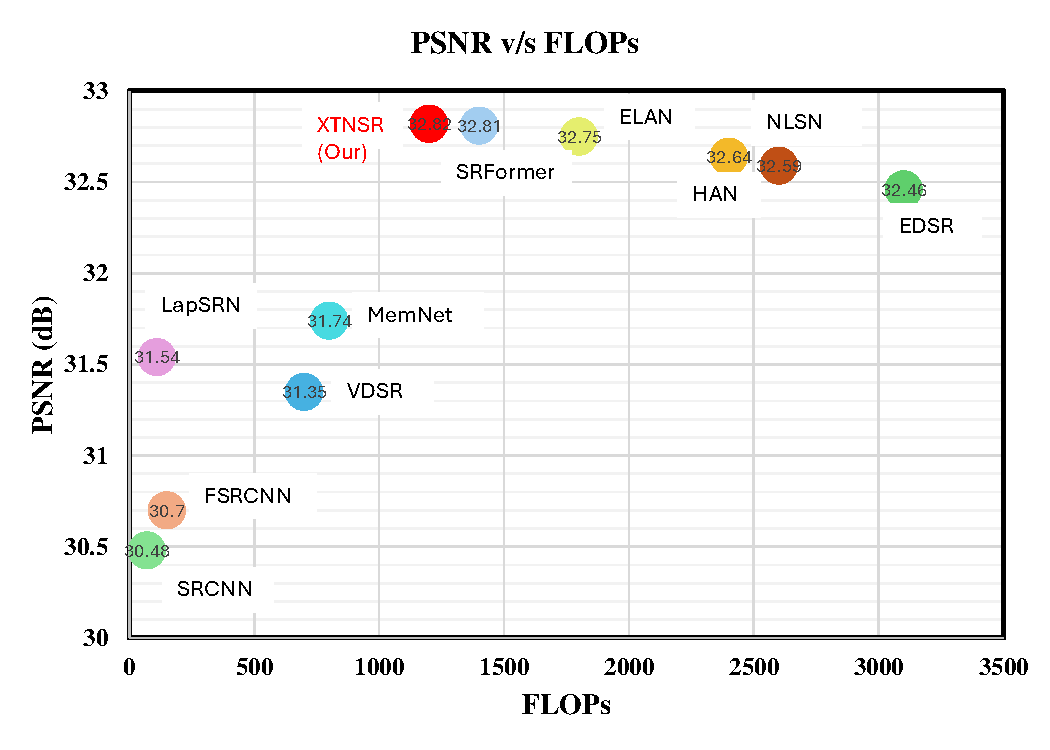
\includegraphics[width=0.5\textwidth]{20FIGURE.pdf}}
   \caption {FLOPs v/s PSNR for Set5 [64] scale ×4.}
    \label{fig:20}
\end{figure}

\subsubsection{Analysis with different window sizes in the Local Feature Window Transformer (LFWT) Block}

To assess the effect of different window sizes, we set the window sizes to be 8 × 8, 16 × 16, and 24 × 24 and compare our proposed model with existing state-of-the-art transformer-based methods like SwinIR [26] and SRFormer [28] on image SR test dataset for up-scaling factor ×4. Table 3 compares our model with other Image SR models evaluated for different window sizes. Larger window sizes increase the super-resolution model's accuracy, as seen from Table 3's quantitative values, our model shows better performance in PSNR and SSIM on publicly available datasets.

\begin{table*}
\centering
\caption{Impact of varying window sizes on performance for $\times$4 upscaling factor. {\color{red}\textbf{Red}} indicates the best quantitative value, whereas the {\color{blue}\underline{blue}} indicates the second-best quantitative value.}
\label{table3}
\setlength{\tabcolsep}{3pt}

\begin{tabular}{|c|c|cc|cc|cc|cc|cc|}
  \hline
  \multirow{2}{*}{Method} & \multirow{2}{*}{Window Size} & \multicolumn{2}{c|}{Set5 [64]} & \multicolumn{2}{c|}{Set14 [65]} & \multicolumn{2}{c|}{BSD100 [66]} & \multicolumn{2}{c|}{Urban100 [67]} & \multicolumn{2}{c|}{Manga109 [68]}   \\
  
\cline{3-12} && \multicolumn{1}{c|}{PSNR}  & SSIM & \multicolumn{1}{c|}{PSNR}  & SSIM  & \multicolumn{1}{c|}{PSNR}  & SSIM  & \multicolumn{1}{c|}{PSNR}  & SSIM & \multicolumn{1}{c|}{PSNR}  & SSIM \\
 \hline
  \multirow{3}{*}{SwinIR [26]} & {8 $\times$ 8}  & \multicolumn{1}{c|}{38.24} &{0.9615}  & \multicolumn{1}{c|}{33.94} &{0.9212} & \multicolumn{1}{c|}{32.39} &{0.9023} & \multicolumn{1}{c|}{33.09} &{0.9373}  & \multicolumn{1}{c|}{39.34} &{0.9784} \\
            & {16 $\times$ 16}   & \multicolumn{1}{c|}{38.32} &{0.9618}  & \multicolumn{1}{c|}{34.00} &{0.9212} & \multicolumn{1}{c|}{\color{blue}\underline{32.44}} &{\color{blue}\underline{0.9030}} & \multicolumn{1}{c|}{33.40} &{0.9394}  & \multicolumn{1}{c|}{39.53} &{0.9791} \\
            & {24 $\times$ 24} & \multicolumn{1}{c|}{38.35} &{0.9620}  & \multicolumn{1}{c|}{34.04} &{0.9214} & \multicolumn{1}{c|}{\color{red}\textbf{32.48}} &{\color{red}\textbf{0.9034}} & \multicolumn{1}{c|}{\color{blue}\underline{33.54}} &{0.9402}  & \multicolumn{1}{c|}{\color{blue}\underline{39.71}} &{\color{red}\textbf{0.9798}}  \\
  \hline
  \multirow{3}{*}{SRFormer [28]} & {8 $\times$ 8}  & \multicolumn{1}{c|}{38.20} &{0.9611}  & \multicolumn{1}{c|}{34.06} &{0.9214} & \multicolumn{1}{c|}{32.36} &{0.9021} & \multicolumn{1}{c|}{32.92} &{0.9361}  & \multicolumn{1}{c|}{39.10} &{0.9777} \\
            & {16 $\times$ 16}   & \multicolumn{1}{c|}{38.31} &{0.9617}  & \multicolumn{1}{c|}{34.10} &{0.9217} & \multicolumn{1}{c|}{32.43} &{0.9026} & \multicolumn{1}{c|}{33.26} &{0.9385}  & \multicolumn{1}{c|}{39.36} &{0.9785} \\
            & {24 $\times$ 24} & \multicolumn{1}{c|}{\color{blue}\underline{38.38}} &{\color{blue}\underline{0.9621}}  & \multicolumn{1}{c|}{\color{blue}\underline{34.13}} &{\color{red}\textbf{0.9228}} & \multicolumn{1}{c|}{\color{blue}\underline{32.44}} &{\color{blue}\underline{0.9030}} & \multicolumn{1}{c|}{33.51} &{\color{blue}\underline{0.9405}}  & \multicolumn{1}{c|}{39.49} &{0.9788}  \\
  \hline
  \multirow{3}{*}{XTNSR (Ours)} & {8 $\times$ 8}  & \multicolumn{1}{c|}{38.26} &{0.9616}  & \multicolumn{1}{c|}{34.08} &{0.9215} & \multicolumn{1}{c|}{32.38} &{0.9020} & \multicolumn{1}{c|}{33.06} &{0.9368}  & \multicolumn{1}{c|}{39.22} &{0.9782} \\
            & {16 $\times$ 16}   & \multicolumn{1}{c|}{38.34} &{0.9620}  & \multicolumn{1}{c|}{34.11} &{0.9217} & \multicolumn{1}{c|}{\color{blue}\underline{32.44}} &{0.9028} & \multicolumn{1}{c|}{33.44} &{0.9398}  & \multicolumn{1}{c|}{39.51} &{0.9793} \\
            & {24 $\times$ 24} & \multicolumn{1}{c|}{\color{red}\textbf{38.40}} &{\color{red}\textbf{0.9622}}  & \multicolumn{1}{c|}{\color{red}\textbf{34.14}} &{\color{blue}\underline{0.9222}} & \multicolumn{1}{c|}{\color{red}\textbf{32.48}} &{\color{red}\textbf{0.9034}} & \multicolumn{1}{c|}{\color{red}\textbf{33.68}} &{\color{red}\textbf{0.9409}}  & \multicolumn{1}{c|}{\color{red}\textbf{39.86}} &{\color{blue}\underline{0.9796}}  \\
  \hline
\end{tabular}
\end{table*}

\subsubsection{Ablation assessment using traditional denoising methods}

In this section, we present a comparative analysis of our XTNSR model applied to the Urban100 [68] Dataset at a scale of ×2 against traditional denoising approaches including Block Matching and 3D Filtering (BM3D) [72], a Fast and Flexible Solution for CNN-Based Image Denoising (FFDNet) [73], Nonlocally Centralized Sparse Representation (NCSR) [74], and Denoising Convolutional Neural Network (DnCNN) [11]. The evaluation is based on PSNR metrics under Gaussian noise with varying noise levels ($\sigma$), specifically $\sigma = 5$, $\sigma = 10$, and $\sigma = 15$, as summarized in Table 4.

\begin{table*}
%\floatsetup{heightadjust=object,valign=t} % Adjust vertical alignment
\centering
\caption{Performance evaluation for noise degradation of images on Urban [68] for scale factor $\times$2. The best quantitative value has been recorded as bold with {\color{red}\textbf{Red }} color. The second best quantitative value is shown in {\color{blue}\underline{blue}} color with an underline.}

\label{table4}
\setlength{\tabcolsep}{1 pt}
\begin{tabular}{|c|c|c|c|c|c|c|c|} % Specify four columns with "c" for centered alignment
\hline

\multirow{1}{*}{Methods / Noise Level} & \multirow{1}{*}{BM3D[72]} & \multirow{1}{*}{FFDNet [73]} & \multirow{1}{*}{NCSR [74]}  & \multirow{1}{*}{DnCNN [11]} & \multirow{1}{*}{XTNSR (Our)}\\

\hline
$\sigma = 5$ & {31.18} & {31.34} & {31.56} & {\color{blue}\underline{31.67}} & {\color{red}\textbf{31.78}}   \\
$\sigma = 10$ & {29.61} & {29.76} & {29.44} & {29.82} & {29.89}   \\
$\sigma = 15$ & {28.12} & {28.48} & {28.64} & {28.58} & {28.77}   \\
    
% Add more rows as needed
\hline
\end{tabular}
\end{table*}

\subsubsection{Ablation assessment using different non-linearity functions in Xception Block}

We changed the ReLU activation to PReLU and CReLU, as seen in Figure 21 in the Xception block of the model. The model was trained for 400 epochs and on scale ×2, and the average PSNR and SSIM were calculated on image test datasets. Table 5 shows that the best PSNR and SSIM are obtained with ReLU activation and the second best with CReLU.

\begin{figure*}
    \centering
    \includegraphics[width=\linewidth]{21Figure.pdf}
    \caption{Xception Block with different non-linearity.}
    \label{fig:21}
\end{figure*}

Figure 22, Figure 23, and Figure 24 show the model's PSNR, SSIM, and Loss convergence with ReLU, CReLU, and PReLU activations, respectively. The values are plotted using the DIV2K [63] training Dataset on the up-scaling factor of ×2 for 100 epochs, keeping other hyper-parameters the same. 

Figure 22 and Figure 23 show that ReLU non-linearity gives better PSNR and SSIM training convergence for the model. Figure 24 presents that ReLU gives minimal loss convergence during training. Henceforth, it is better to use ReLU activation for our proposed XTNSR Network.

\begin{table} 
\caption{Assessment of the Xception block using various activations, such as PReLU, CReLU, and ReLU. The average PSNR and SSIM quantitative values are computed using the Image SR test datasets with an up-scaling factor of $\times2$ across 100 epochs.{\color{red}\textbf{Red }} indicates the best quantitative value, whereas {\color{blue}\underline{blue}} indicates the second-best quantitative value.}
\label{table5}
\setlength{\tabcolsep}{3pt}
\centering
\begin{tabular}{|c|c|c|c|c|c|}
\hline
Non-Linearity       & \multicolumn{3}{c|}{Xception Block}    & Average PSNR               & Average SSIM     \\
\hline
ReLU         & \checkmark & $\times$ &$\times$  &{\color{red}\textbf{32.66}}     &{\color{red}\textbf{0.8876}}  \\
\hline
CReLU          &$\times$& \checkmark& $\times$  & {\color{blue}\underline{32.62}}  & {\color{blue}\underline{0.8872}}      \\
\hline
PReLU          &$\times$& $\times$ & \checkmark  & {32.58}   & {0.8868}  \\

\hline
\end{tabular}
\end{table}

\begin{figure}
    \centering
    \subfloat{\includegraphics[width=0.5\textwidth]{22Figure.pdf}}
    \caption{PSNR convergence using different non-linearity on the DIV2K [63] dataset for up-scaling factor ×2.}
    \label{fig:22}
\end{figure}

\begin{figure}
    \centering
    \subfloat{\includegraphics[width=0.5\textwidth]{23Figure.pdf}}
    \caption{SSIM convergence using different non-linearity on the DIV2K [63] dataset for up-scaling factor ×2.}
    \label{fig:23}
\end{figure}

\begin{figure}
    \centering
    \subfloat{\includegraphics[width=0.5\textwidth]{24Figure.pdf}}
    \caption{Loss convergence using different non-linearity for up-scaling factor ×2.}
    \label{fig:24}
\end{figure}

\subsubsection{Ablation assessment using different non-linearity functions in Multi-Layer Feature Fusion (MLFF) Block}

We did a similar assessment in the Multi-Layer Feature Fusion (MLFF) Block, just as in the Xception Block. We performed experiments by changing the non-linearity in the Multi-Layer Feature Fusion (MLFF) Block. Figure 25 shows the MLFF blocks with different activation functions. The quantitative values shown in Table 6 reveal that ReLU activation gives the best average PSNR and SSIM values of Image SR test datasets. The second-best value is given by CReLU activation.
\begin{figure}
  \centering
  \subfloat{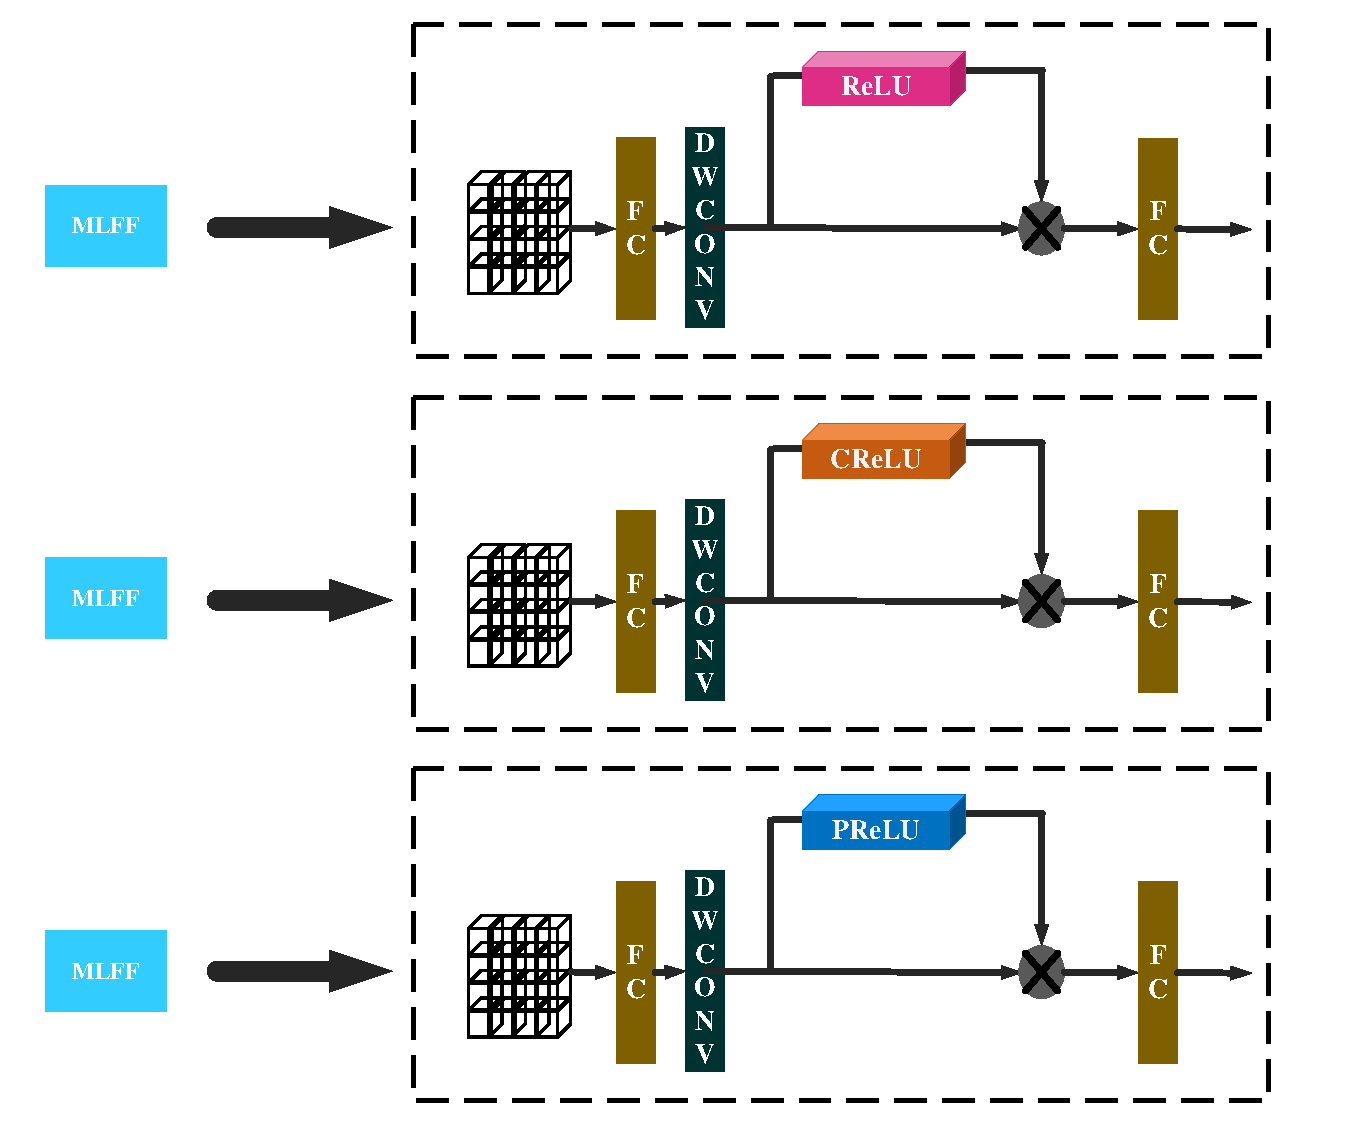
\includegraphics[width=0.5\textwidth]{25FIGURE.pdf}}
   \caption {MLFF Block with different non-linearity.}
    \label{fig:25}
\end{figure}

\begin{table} [h]
\caption{Assessment of the MLFF block using various activations, such as PReLU, CReLU, and ReLU. The average PSNR and SSIM quantitative values are computed using the Image SR test datasets with an up-scaling factor of $\times2$ across 100 epochs. {\color{red}\textbf{Red}} indicates the best quantitative value, whereas {\color{blue}\underline{blue}} indicates the second-best quantitative value.}
\label{table6}
\setlength{\tabcolsep}{3pt}
\centering
\begin{tabular}{|c|c|c|c|c|c|}
\hline
Non-Linearity       & \multicolumn{3}{c|}{MLFF Block}    & Average PSNR               & Average SSIM     \\
\hline
ReLU         & \checkmark & $\times$ &$\times$  &{\color{red}\textbf{32.68}}     &{\color{red}\textbf{0.8879}}  \\
\hline
CReLU          &$\times$& \checkmark& $\times$  & {\color{blue}\underline{32.65}}  & {\color{blue}\underline{0.8876}}      \\
\hline
PReLU          &$\times$& $\times$ & \checkmark  & {32.60}   & {0.8872}  \\

\hline
\end{tabular}
\end{table}

Figures 26, 27, and 28 also show PSNR, SSIM, and loss convergence for the MLFF Block of the model with different ReLU, CReLU, and PReLU activations. The DIV2K [63] training dataset has been used to plot the curves on the up-scaling factor of ×2 for 100 epochs, keeping other hyper-parameters the same.

Figures 26 and 27 show that ReLU shows better PSNR and SSIM versus epoch convergence than CReLU and PReLU. Figure 28 further shows that ReLU gives better loss convergence, proving that ReLU is the most suitable activation to use in our proposed XTNSR model.

\begin{figure}
    \centering
    \subfloat{\includegraphics[width=0.5\textwidth]{26Figure.pdf}}
    \caption{PSNR versus epoch convergence using different non-linearity on the DIV2K [63] dataset for up-scaling factor ×2.}
    \label{fig:26}
\end{figure}

\begin{figure}
    \centering
    \subfloat{\includegraphics[width=0.5\textwidth]{27Figure.pdf}}
    \caption{SSIM versus epoch convergence using different non-linearity on the DIV2K [63] dataset for up-scaling factor ×2.}
    \label{fig:27}
\end{figure}

\begin{figure}
    \centering
    \subfloat{\includegraphics[width=0.5\textwidth]{28Figure.pdf}}
    \caption{Loss versus epoch convergence using different non-linearity for up-scaling factor ×2.}
    \label{fig:28}
\end{figure}


\section{Conclusions and Future Work}

In conclusion, our work presents the XTNSR model, which combines novel Local Feature Window Transformers with Xception blocks for single-image super-resolution. We effectively handle patches to preserve computational efficiency while guaranteeing accuracy using a Patch Embedding layer. We efficiently balance local and global information by combining the LWFT and Xception blocks in a multi-path network backbone. Thus, mitigating over-smoothing and artifact generation. This method also helps to recover noisy images by capturing the hierarchical feature through integrating the Xception Block in the network. The model's efficacy is demonstrated across various up-scaling factors by evaluating five benchmark datasets. A detailed analysis of five benchmark datasets reveals that the suggested XTNSR approach also improves restoration effects concerning both statistical and subjective requirements for up-scaling factors of ×2, ×3, ×4, and ×8. Future research will refine the model for real-time and high-definition video applications.


%\begin{acknowledgements}
%This research is funded by the Second Century Fund (C2F), Department of Electrical Engineering, Faculty of Engineering, Chulalongkorn University Bangkok, 10330, Thailand, and the Ratchadapiseksompotch Fund Chulalongkorn University, Bangkok, Thailand.
%\end{acknowledgements}

\section*{Conflict of interest}
 The authors declare that they have no conflict of interest.

\begin{thebibliography}{00}

\bibitem{b1} J. Greenspan, H., \textit{Super-resolution in medical imaging.} The computer journal, 2009. 52(1): p. 43-63

\bibitem{b2} Lorch, B. and Riess, C., \textit{Image forensics from chroma subsampling of high-quality JPEG images.} In Proceedings of the ACM Workshop on Information Hiding and Multimedia Security. July, 2019. pp. 101-106.

\bibitem{b3} Zhang, Z., Barbary, K., Nothaft, F.A., Sparks, E.R., Zahn, O., Franklin, M.J., Patterson, D.A. and Perlmutter, S.,  \textit{Kira: Processing astronomy imagery using big data technology.} IEEE Transactions on Big Data, 2016. 6(2): pp.369-381.

\bibitem{b4} Ronneberger, O., P. Fischer, and T. Brox. \textit{U-net: Convolutional networks for biomedical image segmentation}. in International Conference on Medical image computing and computer-assisted intervention. 2015. Springer.

\bibitem{b5} Zhang, L., et al., \textit{A super-resolution reconstruction algorithm for surveillance images}. Signal Processing, 2010. 90(3): p. 848-859.

\bibitem{b6} Olsen, S.I., \textit{Estimation of noise in images: An evaluation.} CVGIP: Graphical Models and Image Processing, 1993. 55(4):  p.319-323.

\bibitem{b7} A. Basharat, A. Gritai, and M. Shah, \textit{"Learning object motion patterns for anomaly detection and improved object detection,"} IEEE Conference on Computer Vision and Pattern Recognition, Anchorage, AK, USA, 2008, pp. 1-8, doi: 10.1109/CVPR.2008.4587510.

\bibitem{b8} C. Dong, C. C. Loy, K. He and X. Tang, \textit{"Image super-resolution using deep convolutional networks"}, \textit{IEEE Trans. Pattern Anal. Mach. Intell.}, vol. 38, pp. 295-307, Feb. 2015.

\bibitem{b9} Dong, C., C.C. Loy, and X. Tang. \textit{Accelerating the super-resolution convolutional neural network. in European conference on computer vision}. 2016. Springer.

\bibitem{b10} J. Kim, J. K. Lee and K. M. Lee, \textit{"Accurate image super-resolution using very deep convolutional networks"}, \textit{Proc. IEEE Conf. Comput. Vis. Pattern Recognit.}, pp. 1646-1654, Jun, 2016.

\bibitem{b11} Chen, J. and Li, F., \textit{Denoising convolutional neural network with mask for salt and pepper noise}. IET Image Processing, 2019. 13(13), pp.2604-2613.

\bibitem{b12} W.-S. Lai, J.-B. Huang, N. Ahuja and M.-H. Yang, \textit{"Deep Laplacian pyramid networks for fast and accurate super-resolution"}, \textit{Proc. IEEE Conf. Comput. Vis. Pattern Recognit.}, pp. 5835-5843, Jul. 2017.

\bibitem{b13} Kim, J., J.K. Lee, and K.M. Lee. \textit{Deeply-recursive convolutional network for image super-resolution}. in \textit{Proceedings of the IEEE conference on computer vision and pattern recognition}. 2016.

\bibitem{b14} Tai, Y., Yang, J. and Liu, X., \textit{Image super-resolution via deep recursive residual network}. In \textit{Proceedings of the IEEE conference on computer vision and pattern recognition}, 2017. (pp. 3147-3155).

\bibitem{b15} Y. Tai, J. Yang, X. Liu and C. Xu, \textit{"MemNet: A persistent memory network for image restoration"}, \textit{Proc. IEEE Conf. Int. Conf. Comput. Vis.}, Oct 2017. pp. 4539-4547. 

\bibitem{b16} Ahn, N., Kang, B. and Sohn, K.A., \textit{Fast, accurate, and lightweight super-resolution with cascading residual network.} In Proceedings of the European conference on computer vision (ECCV), 2018. (pp. 252-268).

\bibitem{b17} Lim, B., \textit{Enhanced deep residual networks for single image super-resolution}. in \textit{Proceedings of the IEEE conference on computer vision and pattern recognition workshops}. 2017.

\bibitem{b18} C. Ledig, L. Theis, F. Huszar, J. Caballero, A. Cunningham, A. Acosta, A. P. Aitken, A. Tejani, J. Totz, Z. Wang et al., \textit{Photorealistic single image super-resolution using a generative adversarial network} in CVPR, 2017.

\bibitem{b19} M. S. Sajjadi, B. Scholkopf, and M. Hirsch, \textit{Enhancenet: Single image super-resolution through automated texture synthesis} in ICCV, 2017.

\bibitem{b20} X. Wang, K. Yu, S. Wu, J. Gu, Y. Liu, C. Dong, C. C. Loy, Y. Qiao, and X. Tang, \textit{Esrgan: Enhanced super-resolution generative adversarial networks} in ECCV Workshop, 2018.

\bibitem{b21} Zhang, Y., et al. \textit{Image super-resolution using very deep residual channel attention networks}. in \textit{Proceedings of the European conference on computer vision (ECCV)}. 2018.

\bibitem{b22} Mei, Y., et al. \textit{Image super-resolution with cross-scale non-local attention and exhaustive self-exemplars mining}. in \textit{Proceedings of the IEEE/CVF conference on computer vision and pattern recognition}. 2020.

\bibitem{b23} Mei, Y., Y. Fan, and Y. Zhou. \textit{Image super-resolution with non-local sparse attention}. in \textit{Proceedings of the IEEE/CVF Conference on Computer Vision and Pattern Recognition}. 2021.

\bibitem{b24} Niu, B., Wen, W., Ren, W., Zhang, X., Yang, L., Wang, S., Zhang, K., Cao, X. and Shen, H., 2020. \textit{Single image super-resolution via a holistic attention network}. In \textit{Computer Vision–ECCV 2020: 16th European Conference, Glasgow, UK, August 23–28, 2020, Proceedings, Part XII 16} (pp. 191-207). Springer International Publishing.

\bibitem{b25} Zhang, X., Zeng, H., Guo, S. and Zhang, L., \textit{Efficient long-range attention network for image super-resolution.} In European Conference on Computer Vision (pp. 649-667). Cham: Springer Nature Switzerland, Oct, 2022.

\bibitem{b26} Liang, J., Cao, J., Sun, G., Zhang, K., Van Gool, L. and Timofte, R. \textit{SwinIR: Image restoration using swin transformer}. In \textit{Proceedings of the IEEE/CVF international conference on computer vision}, 2021. (pp. 1833-1844).

\bibitem{b27} Liu, Z., Lin, Y., Cao, Y., Hu, H., Wei, Y., Zhang, Z., Lin, S. and Guo, B. \textit{Swin Transformer: Hierarchical vision transformer using shifted windows.} In Proceedings of the IEEE/CVF international conference on computer vision, 2021. (pp. 10012-10022).

\bibitem{b28} Zhou, Y., Li, Z., Guo, C.L., Bai, S., Cheng, M.M. and Hou, Q. \textit{SRFormer: Permuted Self-Attention for Single Image Super-Resolution.} arXiv preprint, 2023. arXiv:2303.09735.

\bibitem{b29} Dosovitskiy A., Beyer L., Kolesnikov A., Weissenborn D., Zhai X., Unterthiner T., Dehghani M., Minderer M., Heigold G., Gelly S., Uszkoreit J., and Houlsby N. \textit{An image is 11worth 16$\times$16 words: Transformers for image recognition at scale.} In International Conference on Learning Representations, 2021.

\bibitem{b30} Chollet, F. \textit{Xception: Deep learning with depthwise separable convolutions.} In Proceedings of the IEEE Conference on Computer Vision and Pattern Recognition (pp. 1251-1258). 2017.

\bibitem{b31} Mehri, A., Ardakani, P.B. and Sappa, A.D. \textit{MPRNet: Multi-path residual network for lightweight image super-resolution.} In Proceedings of the IEEE/CVF Winter Conference on Applications of Computer Vision, 2021. pp. 2704-2713.

\bibitem{b32} Tong, T., Li, G., Liu, X. and Gao, Q. \textit{Image super-resolution using dense skip connections.} In Proceedings of the IEEE International Conference on Computer Vision, 2017. pp. 4799-4807. 

\bibitem{b33} Trockman, A. and Kolter, J.Z. \textit{Patches are all you need?}.  2022. arXiv preprint arXiv:2201.09792.

\bibitem{b34} Chun-Le G., Yan Q., Anwar S., Cong R., Ren W., and Li C. \textit{Image dehazing transformer with transmission-aware 3d position embedding.} In CVPR, 2022.

\bibitem{b35} Hui, Z., Gao, X., Yang, Y. and Wang, X., \textit{Lightweight image super-resolution with information multi-distillation network}. In \textit{Proceedings of the 27th ACM international conference on multimedia}, October 2019. (pp. 2024-2032).

\bibitem{b36} Li, Z., et al. \textit{Feedback network for image super-resolution}. in \textit{Proceedings of the IEEE/CVF conference on computer vision and pattern recognition}. 2019.

\bibitem{b37} K. Zhang, W. Zuo and L. Zhang, \textit{"Learning a single convolutional super-resolution network for multiple degradations}", \textit{Proc. IEEE/CVF Conf. Comput. Vis. Pattern Recognit.}, Jun. 2018. vol. 6, no. 1, pp. 3262-3271.

\bibitem{b38} K.-W. Hung, Z. Zhang and J. Jiang, \textit{"Real-time image super-resolution using recursive depthwise separable convolution network"}, \textit{IEEE Access}, vol. 7, 2019. pp. 99804-99816.

\bibitem{b39} X. Yang, H. Mei, J. Zhang, K. Xu, B. Yin, Q. Zhang, et al., \textit{"DRFN: Deep recurrent fusion network for single-image super-resolution with large factors"}, \textit{IEEE Trans. Multimedia}, Feb. 2019. vol. 21, no. 2, pp. 328-337.

\bibitem{b40} Wazir M., Aramvith S., and Onoye T. \textit{"SENext: Squeeze-and-ExcitationNext for Single Image Super-Resolution." }IEEE Access (2023).


\bibitem{b41} Z. Wang, J. Chen, and S. C. H. Hoi, \textit{‘Deep learning for image superresolution: A survey.}  IEEE Trans. Pattern Anal. Mach. Intell., vol. 43, no. 10, Oct. 2021. pp. 3365–3387.

\bibitem{b42} Zhang, Y., et al. \textit{Residual dense network for image super-resolution}. in \textit{Proceedings of the IEEE conference on computer vision and pattern recognition}. 2018.

\bibitem{b43} Wang, F., Jiang, M., Qian, C., Yang, S., Li, C., Zhang, H., Wang, X. and Tang, X. \textit{Residual attention network for image classification.} In Proceedings of the IEEE conference on computer vision and pattern recognition, 2017. pp. 3156-3164.

\bibitem{b44} Ruangsang W., Aramvith S., and Onoye T. "Multi-FusNet of Cross Channel Network for Image Super-Resolution." IEEE Access (2023).

\bibitem{b45} Hong, J., Lee, B., Ko, K. and Ko, H. \textit{Fast non-local attention network for light super-resolution.} Journal of Visual Communication and Image Representation, 2023. p.103861.

\bibitem{b46} Dai, T., et al. \textit{Second-order attention network for single image super-resolution}. in \textit{Proceedings of the IEEE/CVF conference on computer vision and pattern recognition}. 2019.

\bibitem{b47} Liu, J., et al. \textit{Residual feature aggregation network for image super-resolution}. in \textit{Proceedings of the IEEE/CVF conference on computer vision and pattern recognition}. 2020.

\bibitem{b48} Prajapati, K., Chudasama, V., Upla, K., Raia, K., Ramachandra, R. and Busch, C. \textit{Channel Split Convolutional Neural Network for Single Image Super-Resolution (CSISR).} In 2021 16th IEEE International Conference on Automatic Face and Gesture Recognition (FG 2021), December 2021. pp. 1-8. 

\bibitem{b49} Park, K., Soh, J.W. and Cho, N.I. \textit{Dynamic residual self-attention network for lightweight single image super-resolution.} IEEE Transactions on Multimedia, 2021.

\bibitem{b50} Zhang, Y., Wei, D., Qin, C., Wang, H., Pfister, H. and Fu, Y. \textit{Context reasoning attention network for image super-resolution.} In Proceedings of the IEEE/CVF International Conference on Computer Vision, 2021. pp. 4278-4287.

\bibitem{b51} Li, Z., Li, G., Li, T., Liu, S. and Gao, W. \textit{Information-growth attention network for image super-resolution.} In Proceedings of the 29th ACM International Conference on Multimedia. October, 2021. pp. 544-552.

\bibitem{b52} Wang, X., Girshick, R., Gupta, A. and He, K. \textit{Non-local neural networks}. In Proceedings of the IEEE conference on computer vision and pattern recognition, 2018. (pp. 7794-7803).

\bibitem{b53} Talreja, J., Aramvith, S. and Onoye, T. \textit{DANS: Deep Attention Network for Single Image Super-Resolution.} IEEE Access, 2023.

\bibitem{b54} Vaswani, A., Shazeer, N., Parmar, N., Uszkoreit, J., Jones, L., Gomez, A.N., Kaiser, Ł. and Polosukhin, I.\textit{Attention is all you need}. Advances in neural information processing systems, 2017. 30.

\bibitem{b55} Wolf, T., Debut, L., Sanh, V., Chaumond, J., Delangue, C., Moi, A., Cistac, P., Rault, T., Louf, R., Funtowicz, M. and Davison, J. \textit{Transformers: State-of-the-art natural language processing.} In Proceedings of the 2020 conference on empirical methods in natural language processing: system demonstrations, October 2020. pp. 38-45.

\bibitem{b56} Malczewski, K. and Stasiński, R. \textit{Super-resolution for multimedia, image, and video processing applications}. In Recent Advances in Multimedia Signal Processing and Communications Berlin, Heidelberg: Springer Berlin Heidelberg, 2009. pp. 171-208.

\bibitem{b57} Chen, Y., Li, Q., Zhang, A., Zou, L., Jiang, Y., Xu, Z., Li, J. and Yuan, Z. \textit{Higher quality live streaming under lower uplink bandwidth: an approach of super-resolution based video coding.} In Proceedings of the 31st ACM Workshop on Network and Operating Systems Support for Digital Audio and Video, July 2021. pp. 74-81.

\bibitem{b58} Isaac, J.S. and Kulkarni, R. \textit{Super-resolution techniques for medical image processing.} In 2015 International Conference on Technologies for Sustainable Development (ICTSD) IEEE, Feb 2015. pp. 1-6.

\bibitem{b59} Kong, Y., Ren, X. and Zhou, R. \textit{Deep learning for image super-resolution and its application in urban security.} In 2nd International Conference on Applied Mathematics, Modelling, and Intelligent Computing (CAMMIC 2022) (Vol. 12259, pp. 1459-1464). SPIE.

\bibitem{b60} Zamfir, E., Conde, M.V. and Timofte, R. \textit{Towards real-time 4k image super-resolution.} In Proceedings of the IEEE/CVF Conference on Computer Vision and Pattern Recognition. 2023. pp. 1522-1532.

\bibitem{b61} Taud, H. and Mas, J.F. \textit{Multilayer perceptron (MLP).} Geomatic approaches for modeling land change scenarios, 2018.  pp.451-455.

\bibitem{b62} Arora, R., Basu, A., Mianjy, P. and Mukherjee, A. \textit{Understanding deep neural networks with rectified linear units.} arXiv preprint, 2016. arXiv:1611.01491.

\bibitem{b63} Agustsson, E.,  Timofte, R. \textit{"NTIRE 2017 Challenge on Single Image Super-Resolution: Dataset and Study."} IEEE Conference on Computer Vision and Pattern Recognition Workshops (CVPRW), (2017). 126-135.

\bibitem{b64} Bevilacqua, M.; Roumy, A.; Guillemot, C.; Alberi-Morel, M.L. \textit{Low-complexity single-image super-resolution based on nonnegative neighbor embedding}. In \textit{Proceedings of the British Machine Vision Conference, Surrey}, UK, 3–7 September 2012.

\bibitem{b65} Zeyde, R.; Elad, M.; Protter, M. \textit{On Single Image Scale-Up Using Sparse-Representations}. In \textit{Proceedings of the International Conference on Curves and Surfaces}, Oslo, Norway, 28 June–3 July 2012; pp. 711–730.

\bibitem{b66} Martin, D.; Fowlkes, C.; Tal, D.; Malik, J. \textit{A database of human segmented natural images and its application to evaluating segmentation algorithms and measuring ecological statistics}. In \textit{Proceedings of the Eighth International Conference On Computer Vision} (ICCV-01), Vancouver, BC, Canada, 7–14 July 2001.

\bibitem{b67} Huang, J.-B.; Singh, A.; Ahuja, N. \textit{Single image super-resolution from transformed self-exemplars}. In \textit{Proceedings of the IEEE Conference on Computer Vision and Pattern Recognition}, Boston, MA, USA, 7–12 June 2015.

\bibitem{b68} Matsui, Y.; Ito, K.; Aramaki, Y.; Fujimoto, A.; Ogawa, T.; Yamasaki, T.; Aizawa, K. \textit{Sketch-based manga retrieval using manga109 dataset}. Multimedia. Tools Appl. 2017, 76, 21811–21838.

\bibitem{b69} J. Li, F. Fang, K. Mei and G. Zhang, \textit{"Multi-scale residual network for image super-resolution"}, \textit{Proc. Eur. Conf. Comput. Vis. (ECCV)}, Sep 2018. pp. 517-532.

\bibitem{b70} Wang, C., Li, Z. and Shi, J., \textit{Lightweight image super-resolution with adaptive weighted learning network}, 2019. arXiv preprint arXiv:1904.02

\bibitem{b71} Haris, M., Shakhnarovich, G. and Ukita, N. \textit{Deep back-projection networks for super-resolution.} In Proceedings of the IEEE conference on computer vision and pattern recognition, 2018. pp. 1664-1673.

\bibitem{b72} Dabov, K., Foi, A., Katkovnik, V. and Egiazarian, K. \textit{Color image denoising via sparse 3D collaborative filtering with grouping constraint in luminance-chrominance space.} In 2007 IEEE international conference on image processing, September 2007. (Vol. 1, pp. I-313). IEEE.

\bibitem{b73} Zhang, K., Zuo, W. and Zhang, L., 2018. \textit{FFDNet: Toward a fast and flexible solution for CNN-based image denoising.} IEEE Transactions on Image Processing, 27(9), pp.4608-4622.

\bibitem{b74} Dong, W., Zhang, L., Shi, G. and Li, X. \textit{Nonlocally centralized sparse representation for image restoration.} IEEE Transactions on Image Processing, 22(4),  2012. pp.1620-1630.


\end{thebibliography}

% Authors must disclose all relationships or interests that 
% could have direct or potential influence or impart bias on 
% the work: 
%
% \section*{Conflict of interest}
%
% The authors declare that they have no conflict of interest.


% BibTeX users please use one of
%\bibliographystyle{spbasic}      % basic style, author-year citations
%\bibliographystyle{spmpsci}      % mathematics and physical sciences
%\bibliographystyle{spphys}       % APS-like style for physics
%\bibliography{}   % name your BibTeX data base

% Non-BibTeX users please use
%\begin{thebibliography}{}
%
% and use \bibitem to create references. Consult the Instructions
% for authors for reference list style.
%
%\bibitem{RefJ}
% Format for Journal Reference
%Author, Article title, Journal, Volume, page numbers (year)
% Format for books
%\bibitem{RefB}
%Author, Book title, page numbers. Publisher, place (year)
% etc
%\end{thebibliography}

\end{document}
% end of file template.tex

